\newif\ifsubmission
%\submissionfalse
\submissiontrue

\documentclass[12pt]{ruthesis}
\usepackage{graphicx}
\usepackage{subcaption}
\usepackage{multirow}
\usepackage{appendix}
\usepackage{url}
\usepackage{algorithm}
\usepackage{algcompatible}
\usepackage{amsmath}
\usepackage{color}
\let\labelindent\relax %to avoid conflict with IEEEtran
\usepackage{enumitem}
\usepackage{listings}
\usepackage{numprint}
\usepackage[bookmarks, hidelinks]{hyperref}
\usepackage[numberedsection]{glossaries}

\npthousandsep{,}\npthousandthpartsep{}\npdecimalsign{.}
\graphicspath{{figs/}}

\definecolor{CommentColor}{RGB}{10,100,10}

\ifsubmission
  \newcommand{\TODO}[1]{}
  \newcommand{\CHANGED}[1]{#1}
\else
  \newcommand{\TODO}[1]{\textcolor{red}{TODO: #1}}
  \newcommand{\CHANGED}[1]{\textcolor{blue}{#1}}
\fi

\newcommand{\remove}[1]{}

\newcommand{\chap}[1]{Chapter~\ref{#1}}
\newcommand{\sect}[1]{Section~\ref{#1}}
\newcommand{\fig}[1]{Figure~\ref{#1}}
\newcommand{\tab}[1]{Table~\ref{#1}}
\newcommand{\alg}[1]{Algorithm~\ref{#1}}

\newcommand{\BigO}[1]{\ensuremath{\mathcal{O}\bigl(#1\bigr)}}

\makeglossaries

\newacronym{pf-sfe}{PF-SFE}{Private-Function SFE}
\newacronym{sfe}{SFE}{Secure Function Evaluation}
\newacronym{gc}{GC}{Garbled Circuit}
\newacronym{oram}{ORAM}{Oblivious Random-Access Machine}
\newacronym{ff}{FF}{Flip-Flop}
\newacronym{mux}{MUX}{Multiplexer}
\newacronym{hdl}{HDL}{Hardware Description Language}
\newacronym{aes}{AES}{Advanced Encryption Standard}
\newacronym{hls}{HLS}{High-Level Synthesis}
\newacronym{aes-ni}{AES-NI}{AES New Instructions}
\newacronym{bmr}{BMR}{Beaver-Micali-Rogoway}
\newacronym{gmw}{GMW}{Goldreich-Micali-Wigderson}
\newacronym{cisc}{CISC}{Complex Instruction Set Computing}
\newacronym{risc}{RISC}{Reduced Instruction Set Computing}
\newacronym{alu}{ALU}{Arithmetic Logic Unit}
\newacronym{utm}{UTM}{Universal Turing Machine}
\newacronym{uc}{UC}{Universal Circuit}
\newacronym{ip}{IP}{intellectual property}
\newacronym{fpga}{FPGA}{Field-Programmable Gate Array}
\newacronym{psi}{PSI}{Private Set Intersection}
\newacronym{cpu}{CPU}{Central Processing Uni}
\newacronym{rsa}{RSA}{Rivest-Shamir-Adleman}
\newacronym{sha}{SHA}{Secure Hash Algorithm}
\newacronym{hbc}{HBC}{Honest-But-Curious}
\newacronym{ot}{OT}{Oblivious Transfer}
\newacronym{cl}{CL}{Combinational Logic}
\newacronym{d-ff}{D-FF}{Data Flip-Flop}
\newacronym{pal}{PAL}{Programmable Array Logic}
\newacronym{asic}{ASIC}{Application-Specific Integrated Circuits}
\newacronym{vhsic}{VHSIC}{Very High Speed Integrated Circuit}
\newacronym{ha}{HA}{Half Adder}
\newacronym{fa}{FA}{Full Adder}
\newacronym{isa}{ISA}{Instruction Set Architecture}
\newacronym{dm}{DM}{Data Memory}
\newacronym{im}{IM}{Instruction Memory}
\newacronym{ram}{RAM}{Random Access Memory}
\newacronym{rom}{ROM}{Read-Only Memory}
\newacronym{pc}{PC}{Program Counter}
\newacronym{sscd}{SSCD}{Simple Sequential Circuit Description}
\newacronym{scd}{SCD}{Simple Circuit Description}
\newacronym{gt}{GT}{Garbled Tables}
\newacronym{ngt}{\#GT}{Number of Garbled Tables}
\newacronym{gtd}{GTD}{Garbled Tables Difference}
\newacronym{mfe}{MFE}{Memory Footprint Efficiency}
\newacronym{cbmc}{CBMC}{ANSI-C Bounded Model Checking}
\newacronym{gpu}{GPU}{Graphics Processing Unit}
\newacronym{dc}{DC}{Design Compiler}
\newacronym{tg}{TG}{TinyGarble}
\newacronym{ansi}{ANSI}{American National Standards Institute}
\newacronym{cordic}{CORDIC}{Coordinate Rotation Digital Computer}
\newacronym{lsb}{LSB}{Least Significant Bit}
\newacronym{msb}{MSB}{Most Significant Bit}
\newacronym{knn}{KNN}{K-Nearest Neighbors}
\newacronym{api}{API}{Application Program Interface}
\newacronym{ise}{ISE}{Integrated Synthesis Environment}
\newacronym{sfdl}{SFDL}{Secure Function Definition Language}
\newacronym{shdl}{SHDL}{Secure Hardware Description Language}
\newacronym{psi-ca}{PSI-CA}{PSI Cardinality}
\newacronym{bram}{BRAM}{Block Random-Access Memory}
\newacronym{lut}{LUT}{Lookup table}
\newacronym{soc}{SoC}{System on a Chip}

\newglossaryentry{arm}
{
  name=ARM,
  description={short for Advanced RISC Machine; is a family of RISC architectures for processors}
}
\newglossaryentry{mips}
{
  name=MIPS,
  description={short for Microprocessor without Interlocked Pipeline Stages; is a family of RISC architectures for processors}
}
\newglossaryentry{tinygarble}
{
  name=TinyGarble,
  description={is a framework introduced in this thesis for two-party secure function evaluation using Yao's garbled circuit protocol}
}
\newglossaryentry{arm2gc}
{
  name=ARM2GC,
  description={is a framework introduced in this thesis for high-level two-party secure function evaluation using Yao's garbled circuit protocol}
}
\newglossaryentry{skipgate}
{
  name=SkipGate,
  description={is an algorithm introduced in this thesis for Yao's garbled circuit protocol to reduce the cost of evaluating sequential circuit}
}

\newglossaryentry{pcf}
{
  name=PCF,
  description={short for Portable Circuit Format, is a framework introduced in \cite{kreuter2013pcf} for high-level two-party secure function evaluation using Yao's garbled circuit protocol}
}
\newglossaryentry{frigate}
{
  name=Frigate,
  description={is a framework introduced in \cite{mood2016frigate} for high-level two-party secure function evaluation using Yao's garbled circuit protocol}
}

\newglossaryentry{netlist}
{
  name=netlist,
  description={is a description of a Boolean circuit through listing its Boolean gates and the dependencies between them}
}
\newglossaryentry{synopsys-dc}
{
  name=Synopsys DC,
  description={short for Synopsys Design Compiler, is a commercial synthesis tool targeting \acrfull{asic}}
}
\newglossaryentry{verilog}
{
  name=Verilog,
  description={is a \acrfull{hdl} standardized as IEEE 1364 and used for designing digital hardwares}
}
\newglossaryentry{vhdl}
{
  name=VHDL,
  description={short for \acrshort{vhsic} Hardware Description Language, is a \acrfull{hdl} used for designing digital hardwares}
}
\newglossaryentry{rdtsc}
{
  name=RDTSC,
  description={is an assembly instruction for x86 processors that is used for measuring \acrshort{cpu} time}
}


\title{\gls{tinygarble}: Efficient, Scalable, and Versatile Privacy-Preserving Computation Through Sequential Garbled Circuit}

\author{Ebrahim M. Songhori}
\department{Electrical and Computer Engineering}
\school{Rice University}
\degree{Doctor of Philosophy}

\committee {
Farinaz Koushanfar, Advisor \\
Professor of Electrical and Computer Engineering \\
University of California, San Diego, CA
\and
Joseph R. Cavallaro, Chair \\
Professor of Electrical and Computer Engineering and Computer Science
Rice University, Houston, TX
\and
Aydin Babakhani\\
Assistant Professor of Electrical and Computer Engineering\\
Rice University, Houston, TX
\and
Dan Wallach\\
Professor of Computer Science and of Electrical and Computer Engineering\\
Rice University, Houston, TX
\and
Ahmad-Reza Sadeghi\\
Professor Computer Science\\
Technische Universit{\"a}t Darmstadt, Darmstadt, Germany
}

\address{Houston, Texas}
\donemonth{March} \doneyear{2017} \makeindex

\begin{document}
  \begin{frontmatter}
   \pagenumbering{roman}
   %\makecover
   \maketitle
   % !TEX root = 0_main.tex
\thispagestyle{empty}
\begin{abstract}
Privacy-preserving computation is a standing challenge central to several modern-world applications which require computing on sensitive data. Secure Function Evaluation (SFE) refers to provably secure techniques aiming to address this challenge by enabling multiple parties to jointly compute an arbitrary function on their private inputs. The most promising two-party SFE method is called the Garbled Circuit (GC) Protocol introduced by Andrew Yao. The protocol is built upon representing the function as a Boolean circuit and encrypting/communicating at logic gate level. Despite several key progresses in GC, efficiency and scalability of the available methods are limited by the naive circuit representation as a directed acyclic graph, and ad-hoc logic optimizations. In this work, we introduce TinyGarble, a novel automated methodology based on logic synthesis techniques for generating optimized Boolean circuits for GC protocol. Moreover, TinyGarble achieves an unprecedented level of compactness and scalability by using a sequential circuit description. The preliminary implementation of benchmark functions using TinyGarble demonstrates a high degree of memory-foot-print compactness as well as improvement in overall efficiency compared to results of existing automated tools. Our sequential description also enables us, for the first time, to design and realize a garbled processor to reduce the problem of private function evaluation to a conventional SFE problem. In addition, the garbled processor allows to develop applications in high-level languages and securely evaluate them which eliminates the need for Boolean circuit generation.
\end{abstract}

   % !TEX root = 0_main.tex
\chapter*{Acknowledgements}
\thispagestyle{empty}

I like to acknowledge ...

\clearpage

   \tableofcontents
   \listoffigures
   \listoftables
   % !TEX root = 0_main.tex
\begin{dedication}
To my fianc\'ee, Zeinab.
\end{dedication}

  \end{frontmatter}
\pagenumbering{arabic}

\linespacing{1.7}

% !TEX root = 0_main.tex
\chapter{Introduction}
%what are SFE and GC
Secure Function Evaluation (SFE) allows two or more parties to evaluate an arbitrary function on their private data.
The parties learn the output of the function without revealing any information about their private data.
An important special case of SFE is for two-party, Alice and Bob, want to find $f(a, b)$ where $a$ and $b$ are Alice's and Bob's private inputs respectively and $f(., .)$ is a predetermined arbitrary function.
By far the most promising and efficient solution for two-party SFE is Yao's Garble Circuit (GC) protocol that was proposed by Andrew C. Yao in his seminal work \cite{yao1986generate}.
The GC protocol requires the function $f(., .)$ to be represented in a Boolean circuits consisting of binary gates (e.g., AND, OR, and XOR).
In the GC protocol, Alice encrypts the circuits and Bob decrypts it to learn the output.
The input and intermediate values in the circuit are masked such that no party can gain any information about the private inputs.
Secure evaluating of a Boolean circuit can also be generalized to multi-party SFE \cite{goldreich1987play, ben2008fairplaymp}.

%What has been done?
A host of privacy preserving and security critical applications can directly benefit from a practical and efficient realization of SFE, including but not limited to: biometrics matching, face recognition, image/data classification, electronic auctions and voting, remote diagnosis, secure search, and stable matching \cite{riazi2017toward, zhang2016robust, bringer2013privacy, evans2011efficient, barni2009secure, naor1999privacy, brickell2007privacy, jha2008towards}.
For a few decades after its introduction, the GC protocol had been thought to be too expensive to be practically feasible.
Firplay \cite{malkhi2004fairplay} was the first implementation of the GC protocol that paved the way for later theoretical, algorithmic, and tool developments that have significantly improved the efficiency and practicality of the GC protocol until today, see \cite{malkhi2004fairplay, kolesnikov2008improved, pinkas2009secure, huang2011faster, bellare2013efficient, zahur2015two, zahur2015obliv, liu2015oblivm}.

%what is the problem of circuit generation?
One of the most challenging part of realization of the GC protocol is generating the Boolean circuit for the underlying function $f(., .)$ in SFE.
The function is usually described by users in high-level languages and is translated into a Boolean circuit with binary gates.
The main objective of the GC circuit generation is to create a logically equivalent Boolean circuit with minimum number gates such that its secure evaluation incurs minimum cost.

%classification of the work
The previous work on circuit generation for the GC protocol can be roughly classified into two groups.
One approach is based on building a custom library for a general purpose programming language such as Java along with functions for emitting the circuit, e.g., \cite{huang2011faster,malka2011vmcrypt,henecka2013faster}.
For better usability, these libraries typically include frequently used modules such as adders and multipliers.
However, library-based approaches require manual adjustment and do not perform global circuit optimization.
Moreover, their memory management gets complicated when the number of gates is large thereby affecting performance and scalability \cite{henecka2013faster}.

The second approach is to write a new compiler for a higher-level language that translates the instructions into the Boolean logic, e.g., \cite{malkhi2004fairplay,kreuter2012billion,kreuter2013pcf,franz2014cbmc}.
Although compiler-based approaches can perform global optimizations, they often unroll the circuits into a large list of gates.
For example, the description of a circuit with one billion gates has at least size $2 \log_2 (10^9) \cdot 10^{9} \approx 7$~GB.
To reduce circuit description size, the compiler proposed in \cite{kreuter2013pcf}, called PCF (Portable Circuit Format), does not unroll the loops in the circuit until the GC protocol runs, and therefore seems to have a better scalability than the other compilers.
As we elaborate in related work (see \sect{sect:related}), the existing approaches, including the above proposals, have certain limitations when it comes to real implementation.

Our approach, TinyGarble, is based on synthesizing and optimizing circuits for the GC protocol as sequential circuits while leveraging powerful logic synthesis techniques with our newly introduced custom-libraries.

Our solution simply views the circuit generation for GC as an atypical logic synthesis task that, if properly defined, can still be addressed by conventional hardware synthesis tools.
By posing the circuit generation for Yao's protocol as a hardware synthesis problem, TinyGarble naturally benefits from the elegant algorithms and powerful techniques already incorporated in existing logic synthesis solutions, see, \cite{sentovich1992sis,micheli1994synthesis,devadas1994logic,brayton1987mis}.
This view provides a radically different perspective on this important problem in contrast to the earlier work in this area that attempted to generate circuits by building new libraries for general purpose languages such as Java \cite{huang2011faster,malka2011vmcrypt}, custom compilers such as \cite{kreuter2013pcf,franz2014cbmc}, or introduction of new programming languages such as \cite{malkhi2004fairplay,rastogi2014wysteria}.

TinyGarble introduces new techniques for minimizing the number of non-XOR gates which directly results in reduced computation and communication required for the GC protocol.
We do so by integrating the cost function in the new custom libraries that we design and use within our logic synthesis flow.
This way, we are able to gain up to $80\%$ improvement in the number of non-XOR gates for benchmark circuits compared to PCF \cite{kreuter2013pcf}.
The TinyGarble methodology is automated, i.e., the savings can be achieved for many functions synthesized by our method, regardless of their sophistication.

One significant contribution of TinyGarble, which differentiates it from the previous work, is expressing the function in a very compact format, namely as a sequential logic.
The earlier work in this area mainly described functions in a combinational format, where the value of the output is determined entirely by the circuit inputs.
This input/output relationship can be expressed by a (combinational) Boolean function and a directed acyclic graph (DAG) of binary gates.
The sequential circuit description, on the other hand, allows having feedback from the output to the input by adding the notion of a state (memory).
At each \emph{sequential cycle}, the output of the circuit is determined by the current state of the system and the input.
For each particular sequential cycle, the relationship between the output and the inputs for the given states can be determined as a Boolean combinational logic.

The only previous work we are aware of which implicitly hinted at the possibility of having a more compact representation is PCF \cite{kreuter2013pcf}.
It does so by embracing loops and unrolling them only at runtime.
A sequential circuit, however, goes far beyond the loop embracing performed at the software level.
Not only does TinyGarble embrace the high-level loops, it also enables the user to further compact the functions by folding the implementation up to its basic elements.
For example, using TinyGarble, user can compress the 1024-bit addition function into only a 1-bit adder.

An important advantage of our sequential representation is providing a new degree of freedom to the user to fold the functions to simpler computing elements; i.e., the user has the freedom to choose the number of sequential cycles needed for evaluation of the function--the size of the combinational logic path between the states/inputs and the outputs.
The number of gates in the sequential circuit can be managed by varying the number of cycles.
The memory footprint of the GC operation is directly related to the number of gates in the sequential circuit; at any moment during garbling, only the information corresponding to the current cycle needs to be stored.
Compact sequential circuits yield a small enough memory footprint that can fit mostly on a typical processor cache.
This helps us to avoid costly cache misses while accessing the wire tokens during the GC protocol.
Indeed, TinyGarble can enable practicable embedded implementations with a small memory footprint.

The sequential representation enables, for the first time, implementation of a universal processor for private function evaluation where the function is known only to one party.
We reduce private function SFE (PF-SFE) to general SFE where the function is known by both parties.
Our implementation accepts assembly instructions of the private function as input to the GC protocol.
Since a processor is inherently a sequential circuit, it was infeasible to be realized with previous GC tools.

TinyGarble accepts inputs in two different formats: a standard hardware description language (HDL), or a higher level language as long as it is compatible with the existing high level synthesis (HLS) tools, e.g., the C language for  SPARK \cite{Gupta2004} and Xilinx Vivado \cite{tool:Vivado}, or Python for PandA \cite{tool:PandA}, that converts the high level language to an HDL.
Beside user's manual optimization, TinyGarble performs various optimizations through standard HDL synthesis tools to generate an optimized \emph{netlist}, i.e., list of gates, which is then transformed to be used with a GC protocol implementation, e.g., JustGarble \cite{bellare2013efficient} or Half Gates \cite{zahur2015two}.

%%%%%

Secure Function Evaluation (SFE) allows two (or more) mistrusting parties to jointly compute an arbitrary function on their private inputs without revealing information but the result. The seminal work of Yao \cite{yao1986generate} has introduced the concept of two-party SFE using the Garbled Circuits (GC) protocol which requires that the function is represented as a Boolean circuit. While the GC protocol was originally thought to be of theoretic interest only, algorithmic and implementation optimizations have significantly improved its efficiency during the last decades. In addition to the advances in computing platforms, the key enablers for the progress include newer cryptographic constructs, logic-level transformations, and software techniques.

Compilers for SFE have been continually evolving. A number of compilers~\cite{malkhi2004fairplay,ben2008fairplaymp,henecka2010tasty,kreuter2012billion} translate a functionality written in a domain-specific input language into a Boolean circuit, also described in an intermediate language, which is then evaluated with Yao's GC protocol. Other compilers \cite{franz2014cbmc,kreuter2013pcf} use a subset of the C language as input. However, these methods imply building software-to-Boolean circuit compilers from scratch and often put limitations on the functionality. Moreover, verifying the correctness of these compilers is challenging \cite{mood2016frigate}.

Recently, it was shown that the long-established and verified hardware synthesis compilers can be used for generation of Boolean circuits for SFE, eliminating the need for building ad-hoc logic compilers or tedious handcrafting of Boolean circuits. Another key advantage of conventional logic synthesis is allowing a \emph{sequential logic description} which can be adapted to map general functionalities to Boolean circuits optimized for Yao's GC protocol. The approach was introduced in \cite{songhori2015tinygarble} and shown to yield great improvements in terms of memory and communication. A fully-automated toolchain which utilizes existing logic synthesis compilers and can be generalized for other SFE protocols was presented in \cite{demmler2015automated}. This latter work takes advantage of the built-in intellectual property (IP) and custom design libraries which can be readily adapted during circuit synthesis to realize a broad suite of applications optimized for SFE.

The authors in \cite{songhori2015tinygarble} leverage the capability of synthesizing a sequential circuit and introduce the idea of a general-purpose sequential processor for private function SFE (PF-SFE) by GC, where both input data and function are private. PF-SFE is useful for scenarios where the function is proprietary or classified, e.g., credit checking or private database queries. Their so-called \emph{garbled processor} allows to use existing software compilers for describing the function and generates compatible machine code which is also garbled. A partial implementation of a MIPS processor is provided in \cite{songhori2015tinygarble} which only considers PF-SFE where the entire processor circuit and Instruction Set (IS) have to be garbled in each instruction step during SFE in order to hide the executed instructions in the private function. This results in a tremendous cost compared with SFE for public functions. Thus, their MIPS processor incurs an unnecessary overhead for numerous applications in which a private function is not required. (The only benchmark presented in \cite{songhori2015tinygarble} is the Hamming distance function.)

We propose GarbledCPU, the first configurable hardware-based general purpose sequential CPU for SFE. The FPGA realization of GarbledCPU is based on the MIPS instruction set. GarbledCPU provides a generalized support for SFE of varying flavors of privacy, beyond PF-SFE, to allow for more relaxed privacy demands and hence an improved performance. More explicitly, with GarbledCPU the parties can evaluate a private, semi-private or public function by revealing none, partial or all information about the function respectively while still benefiting from the simplicity of programming a processor.
Both parties decide first which subset of IS they are willing to use which determines the level of privacy ensured. The function is compiled from a high-level language, e.g., C/C++ into assembly code of the agreed upon IS. Next, the garbled processor is securely evaluated given users' garbled input and the compiled function instructions (also garbled) to compute the output.

A recent technical report \cite{wang2015secure} also suggests a secure computation framework using MIPS code. The approach relies on garbled universal circuits to emulate the execution of each instruction of the MIPS program and on Oblivious RAM (ORAM) for memory access. They propose using static analysis of functions to reduce the set of instructions to be garbled. However, \cite{wang2015secure} only presents a software SFE implementation, while we present the first practical hardware sequential processor for both SFE and PF-SFE. An earlier hardware implementation of GC was reported in \cite{jarvinen2010garbled} but the approach only addresses SFE with no support for function hiding and is limited to combinational Boolean circuit as it predated \cite{songhori2015tinygarble}. A combinational description limits usability and scalability and is impractical for control-intensive functions such as CPUs that need to be expressed sequentially.

%%%%%

Secure Function Evaluation (SFE) allows two or more parties to compute an arbitrary joint function such that they learn the function output without revealing their private inputs.
The first and by far the most efficient method for two-party SFE is Yao's Garbled Circuit (GC) protocol~\cite{yao1986generate}.
Yao's protocol immediately attracted a significant attention from the cryptography community, but was believed to be of limited practical usage for many years.
The critical challenge of GC was to generate an optimized Boolean circuit representing the function such that its secure evaluation incurs the minimum communication and encryption cost.

The GC logic optimization challenge was recently addressed by TinyGarble~\cite{songhori2015tinygarble}.
Even though the circuit is just a Boolean representation to be used in GC, a software protocol, TinyGarble showed that the circuit generation can be viewed as an atypical instance of the conventional logic synthesis task.
This approach outperforms previous methods for generating Boolean circuit using custom compilers~\cite{malkhi2004fairplay,holzer2012secure, rastogi2014wysteria,demmler2015aby,liu2015oblivm,mood2016frigate}.
A major disadvantage of TinyGarble, however, is that the efficiency can only be achieved when the function is described in a Hardware Description Language (HDL), e.g., Verilog, instead of a high-level programming language.
Even when they used the best high-level synthesis compiler, i.e., Vivado HLS ~\cite{tool:Vivado}, they lost the HDL efficiency.
In this paper, our goal is to combine the efficiency of hardware synthesis with the versatility of high-level languages.

Recently, a number of researchers proposed the idea of \textit{garbled processor} where the underlying Boolean circuit in GC is that of a general-purpose processor~\cite{wang2015secure, songhori2016garbledcpu}.
This way, users can develop the secure function in a high-level language and feed the compiled binary code to the processor along with their private inputs.
However, the large overheads of such approaches compared with the classic HDL synthesis raises questions about their practicality.
We believe that the primary reason behind the overhead is that they perform coarse-grain (instruction-level) optimization.
At each cycle, they generate a custom processor supporting only the instruction(s) to be executed at that cycle.

In this work, we introduce a methodology to perform fine-grain (gate-level) optimization on garbled processor such that only the gates associated to the private inputs incur garbling cost.
Our key observation is that the gates whose outputs are independent of the private data (and thus known to both parties) can either be computed without communication and encryption or simply skipped.
This observation gives birth to the novel SkipGate algorithm.
The algorithm wraps around the GC protocol to compute the gate outputs that can be computed without communication and to mark the redundant gates for skipping\footnote{SkipGate avoids garbling redundant gates and is orthogonal to cryptographic methods such as Free XOR~\cite{kolesnikov2008improved} and Half Gate~\cite{zahur2015two} that reduce the garbling cost of a gate.}.

SkipGate is mostly effective for reducing the garbling cost of sequential circuits~\cite{songhori2015tinygarble} containing known control paths.
An example of such a circuit is the garbled processor where the control path depends on the binary code of the function that is known to both parties.
By utilizing this property, we develop a high-level GC framework called ARM2GC built upon the ARM instruction set and the SkipGate algorithm.
Users can develop the secure function in high-level languages, e.g., C/C++ and compile it using standard ARM cross-compilers.
In contrast to the earlier custom high-level compilers which called for new ad-hoc verification techniques~\cite{rastogi2014wysteria,demmler2015aby,liu2015oblivm,mood2016frigate}, ARM2GC inherits the ARM's available fully verified compilers.
Thanks to SkipGate, ARM2GC incurs a garbling cost comparable to the HDL synthesis approach of TinyGarble while allowing users to develop SFE applications in a high-level language.

Our work leverages ARM as the general purpose processor, in contrast to the earlier MIPS-based garble processors~\cite{songhori2015tinygarble, wang2015secure, songhori2016garbledcpu} because of ARM's pervasiveness and, most importantly, conditional execution.
The latter simplifies the framework by reducing conditional branches and making the program flow predictable for both parties to take the full advantage of the SkipGate algorithm.
We modify the standard ARM architecture (without affecting the instruction set) such that SkipGate is more effective on the circuit.

\section{Contributions}
In brief, our contributions are as follows:
\begin{itemize}
\item We propose the first hardware-only solution for 2-party GC-based secure sequential function computation with different SFE flavors that allows leveraging the trade-off between privacy and performance: application-specific IS for SFE (\sect{ssect:sfe}), restricted IS (\sect{ssect:semi-pf}) for semi-private SFE, and full IS (\sect{ssect:pfsfe}) for PF-SFE.
\item We realize a proof-of-concept FPGA implementation which demonstrates the feasibility of the sequential garbled processor in hardware, and motivates further research in this direction. GarbledCPU achieves efficiency and performance by leveraging the most recent optimizations for GC \cite{kolesnikov2008improved,bellare2013efficient,zahur2015two,songhori2015tinygarble}, along with a high-throughput pipelined GC evaluation on FPGA. It outperforms the fastest software implementation in the literature which relies on the Intel AES-NI \cite{bellare2013efficient}.
\item We extensively benchmark more complex functions such as AES, Private Set Intersection (PSI), and Hamming distance and evaluate them under our different privacy settings using our framework and when applicable, compare our performance with prior work.
\item We introduce the novel SkipGate algorithm that avoids redundant garbling by utilizing the mutual knowledge between the two parties.
\item
  Adaption of established HDL synthesis techniques to compile and optimize a function into a netlist of gates for use in secure computation protocols.
\item
  Creation of new custom libraries and setting objectives/ constraints to \emph{repurpose} standard synthesis tools for minimizing the number of non-XOR gates in a circuit.
\item
  Introduction of sequential circuit description for achieving an unprecedented compactness in function representation and memory footprint.
\item
  Providing a new degree of freedom to users to fold the functions into a sequential circuit.
  The user can achieve a small enough sequential circuit such that the memory required for its secure evaluation fits even in a typical processor cache.
  This helps to avoid costly cache misses and reduces the CPU time required for GC.
\item
  Proof-of-concept implementation of benchmark functions such as multiplication, and Hamming distance demonstrates up to 5 orders of magnitude savings in memory footprint and up to $80\%$ efficiency in minimizing the total number of non-XOR gates.
  Furthermore, TinyGarble enables implementation of large circuits that were not reported in earlier work, such as SHA-3.% and RSA-8192.

\item
  Implementing the first scalable emulation of a universal processor for private function evaluation where the number of instruction invocations is not limited by the memory required for garbling.
  This design is uniquely enabled by the TinyGarble sequential description.
  Our design is a secure general purpose processor based on the MIPS~I instruction set that receives as inputs the private function from one party and the data from the other.
\item We develop the ARM2GC framework based on the SkipGate algorithm and ARM processor.
    In this framework, users can efficiently develop SFE applications in a high-level language like C/C++.
    It enables them to benefit from the available fully verified compilers of ARM.
    We modify the ARM architecture (without affecting the instruction set) to make it most effective for the GC protocol with SkipGate.
\item We perform extensive experiments to evaluate the SkipGate algorithm and the ARM2GC framework.
    The ARM2GC framework demonstrates comparable performance to HDL synthesis approach of TinyGarble~\cite{songhori2015tinygarble}.
    Its overhead is negligible for most of the benchmark functions and has the maximum value of 6\%.
    As expected, it outperforms the state-of-the-art garbled processors~\cite{wang2015secure, songhori2016garbledcpu} and high-level GC compilers~\cite{holzer2012secure, mood2016frigate}.
\end{itemize}

what we explained in hardware synthesis can be expand to other methods such GMW as shown in ~\cite{} however in this thesis we focus on the GC protocol.

\section{Global Flow}
The global flow of TinyGarble framework is shown in \fig{fig:globalflow}.
The framework consists of two main part (i) GC synthesis and (ii) GC engine.
The GC synthesis flow receives a function description in HDL and generates a circuit description that can be efficiently evaluated by the GC engine.
The GC synthesis can generate combinational circuits as well as sequential ones.

The GC engine allows two parties, Alice and Bob, to securely evaluate the function given the function description generated by the GC synthesis flow.
The engine is an implementation of Yao's GC protocol in C++ and is developed based on JustGarble \cite{bellare2013efficient}.
Our GC engine supports communication which was missing in JustGarble.
It also includes implementation of Half Gate \cite{zahur2015two}, the most recent theoretical optimization on the GC protocol that reduces the communication and computation cost by 33\%.
Also most importantly, our GC engine supports garbling/evaluating of sequential circuits.

\begin{figure}[ht]
\centering
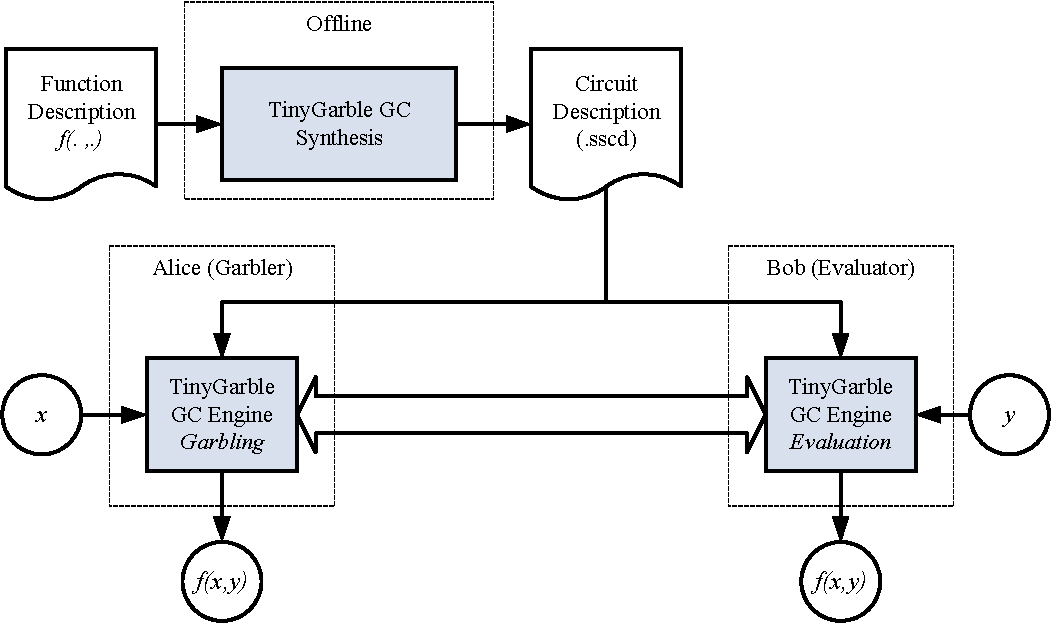
\includegraphics[width=0.7\textwidth]{tinygarble_flow-crop.pdf}
\caption{The global flow of TinyGarble framework.
The framework consists of GC synthesis flow and GC engine.
The GC synthesis flow generates the optimized circuit description given a function.
The GC engine allows two parties (Alice and Bob) to securely compute the function according to Yao's GC protocol.
}
\label{fig:globalflow}
\end{figure}

\section{Organization}

% !TEX root = 0_main.tex
\chapter{Preliminaries and Background}
In this chapter,
-we provide general background information about secure multi-party computation
-we also introduce the generalized problem of secure function evaluation (SFE). and it two-party version and the threat model.
-Then we explain the Yao's Garbled Circuit protocol that enables two-party SFE for honest-but-curios adversary.
-We also explain the theoretical advancement and optimization on the protocol.
-Then we explain basics about combinational and sequential Boolean circuits.

\section{Secure Multi-party Computation}
the general problem of secure multi-party computation:
We have mutually suspicious parties that each has a private attribute (e.g., salary) and wish to compute a joint function (e.g., ) on their attributes.
They have to use some distributed protocol to evaluate and learn the output of the function without leaking their private information to other parties.
If we could find a third party that all the individuals trust, they could give her the inputs and she computes the function and returns the result to the parties.
Of course such a trusted party cannot be found in real scenarios of distributed systems.
Thus at best, we can emulate such a trusted third party with a cryptographic protocol~\cite{goldreich2013general}.
\fig{fig:multi-party-model} shows the idea model with a trusted third party and its emulation in a real model using a secure multi-party computation protocol.

\begin{figure}[ht]
    \centering
    \begin{subfigure}[tl]{0.35\textwidth}
        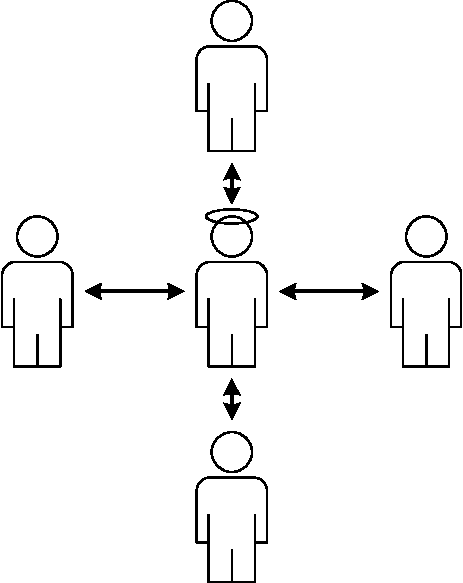
\includegraphics[width=\textwidth]{emulate_ideal-crop.pdf}
        \caption{Ideal Model}\label{fig:ideal-model}
    \end{subfigure}
		~~~~
    \begin{subfigure}[tr]{0.35\textwidth}
        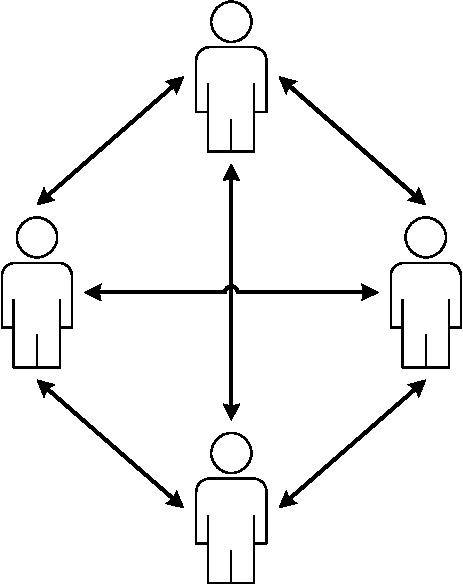
\includegraphics[width=\textwidth]{emulate_real-crop.pdf}
        \caption{Real Model}\label{fig:real-model}
    \end{subfigure}\\
    \caption{Emulation of a trusted third-party in secure multi-party computation (schematic based on~\cite{goldreich2013general}).}\label{fig:multi-party-model}
\end{figure}

Such emulation is possible under assumption about the emulation such as security level and type of the function that can be evaluated.
Initial general protocols Yao's Garbled Circuit Protocol GMW that are able to evaluate general functions.
Homomorphic encryption and Shamir's secret sharing are able to evaluate special function such as addition and multiplication.
In this thesis, we focus on the general secure multi-party computation where arbitrary desired function can be evaluated by the protocol.

\section{Secure Function Evaluation Definition}
The general secure multi-party computation is also known as secure function evaluation (SFE). It can be defined as follow: p parties each have an attribute: i1, ... ip. They want to compute function o = f(i1,i2, .. ip) where o is a tuple (o1, o2, ..., op) such that ok belongs to the kth party.
the function f can also be described as a tuple of functions f = (f1, f2, ...,  fp) where the output of fk(p1, p2, .. pm) = ok belongs to kth party.
(A common special case is that fi's are the same and all parties revives the same output. For example in case of the average of salaries, the result of the average function is evaluated and shared with all the participating parties).

\section{Two-Party Secure Function Evaluation}
two-party SFE is an important special case of general secure multi-party computation that was solved initially by Andrew Yao and GMW.
There are two parties Alice and Bob each has an input a and b and they want to compute (o1, o2) = (f1(a,b), f2(a,b)) where o1 belong to Alice and o2 belongs to Bob.

\begin{figure}[ht]
\centering
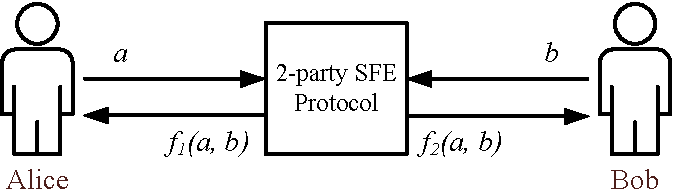
\includegraphics[width=0.70\textwidth]{two_party_SFE-crop.pdf}
\caption{The two-party secure function evaluation (SFE) protocol.}
\label{fig:globalflow}
\end{figure}

\section{Adversary Model}
We assume that all the parties are semi-honest which means that they follow the protocol exactly as specified without deviation or malicious behavior but they try to learn as much as possible about the other party's input from the information they receive during the protocol.
This model is often called honest-but-curious (HBC) adversary model in the literature and it is the basis for building a stronger security protocol.

In related work chapter \ref{ch:related}, we mention some of the recent approaches to extend the adversary model for two-party SFE to make it secure against the malicious adversary who can deviate from the protocol.

\section{Yao's Garbled Circuit Protocol}
Yao introduced the GC protocol for 2-party Secure Function Evaluation (SFE) in the 1980's \cite{yao1986generate}.
GC is described as a circuit whose wires carry a string valued-token instead of a bit.
Consider two parties, Alice and Bob, who want to evaluate a function $f(\cdot)$ without revealing their inputs to each other.
The function needs to be represented as a combinational Boolean circuit.
To begin with, we assume the circuit consists of a single gate with two input wires, $w_{a}$, $w_{b}$ and one output wire $w_{c}$.
Alice knows the value of input $w_{a}$ denoted by $v_{a}$ and Bob knows the value of input $w_{b}$ denoted by $v_{b}$.
The gate is also represented by a four-entry truth table $G[v_{a}, v_{b}]$.
There are two main phases in Yao's protocol.
First, Alice encodes or garbles the circuit by generating garbled tables.
Second, Bob evaluates the output denoted by $v_{c}$ without knowing anything about $v_{a}$ other than what can be deduced from the output and his own input.

The steps of Yao's approach are described below.

\begin{enumerate}
\item
	For each wire $w_a$, Alice selects one random bit $t_a$ called \emph{type} and two random $(k-1)$-bit values $Y_a^{0}$ and $Y_a^{1}$, where $k$ is a symmetric security parameter (e.g., $k=128$).
	The concatenations of the first random string and the type $X_a^{0} =  Y_a^{0}\parallel t_a$ and $X_a^{1} =  Y_a^{1}\parallel \bar{t}_a$ are called token for semantic bit $0$ and $1$ respectively.

\item
	For each gate, Alice symmetrically encrypts the respective output tokens with the four possible combinations of the input tokens.
	The resulting table of ciphertexts is called \emph{garbled table}.

\item
	Alice sends to Bob the garbled tables and the token corresponding to her input value.

\item
	Bob obliviously receives the tokens corresponding to his input through oblivious transfer (OT) \cite{rabin2005exchange}.

\item
	Bob decrypts the corresponding entry in the garbled table based on the received input tokens and gets the output token.

\item
	Finally, Alice reveals the type of the output and Bob determines its semantic value.
\end{enumerate}

In general, the circuit consists of multiple gates.
Yao's protocol for this case is described below.

\begin{enumerate}
\item
	Alice chooses tokens for all the wires, constructs the garbled tables for each gate and sends these to Bob along with the tokens corresponding to her inputs.
\item
	Bob obliviously receives the tokens corresponding to his input values through oblivious transfer.
\item
	Using these tokens, Bob evaluates the circuit gate-by-gate until he evaluates all gates.
\item
	Finally, Alice reveals the type of the outputs and Bob determines their semantic values.
\end{enumerate}

\section{Advancements on the GC Protocol}
In our implementation, we make use of state-of-the-art optimizations for garbled circuits as described below.

\subsection{Free XOR~\cite{kolesnikov2008improved}}
In this method, Alice generates a global random ($k-1$)-bit value $R$ which is just known to her.
During garbling operation for any wire $w_a$, she only generates a token $X_a^{0}$ and computes the other token $X_a^{1}$ as $X_a^{1} = X_a^{0} \oplus (R \parallel 1)$.
With this convention, the token for the output wire of the XOR gates with input wires $w_{a}$, $w_{b}$ and output wire $w_{c}$ can be simply computed as $X_{c} = X_{a} \oplus X_{b}$.
The proof of security for this optimization is given in \cite{kolesnikov2008improved}.

\subsection{Row Reduction~\cite{naor1999privacy}}
This optimization reduces the size of the tables for the non-XOR gates by $25\%$.
Here, instead of generating a token for the output wire of a gate randomly, the output token is produced as a function of the tokens of the inputs.
Alice generates the output token such that the first entry of the garbled table becomes all $0$ and no longer needs to be sent.

\subsection{Garbling With a Fixed-key Block Cipher~\cite{bellare2013efficient}}
This method allows to efficiently garble and evaluate non-XOR gates using fixed-key AES.
In this garbling scheme which is compatible with the Free XOR and Row Reduction techniques, the output key $X_{c}$ is encrypted with the input token $X_{a}$ and $X_{b}$ using the encryption function $E(X_a,X_b,T,X_c) = \pi(K) \oplus K \oplus X_c$, where $K=2X_a\oplus4X_b\oplus T$, $\pi$ is a fixed-key block cipher (e.g., instantiated with AES), and $T$ is a unique-per-gate number (e.g., gate identifier) called \emph{tweak}.
The proof of security is given in~\cite{bellare2013efficient}.



\section{Boolean Circuits}
\subsection{Combinational Boolean Circuits}
\subsection{Sequential Boolean Circuits}

% !TEX root = 0_main.tex
\chapter{Garbled Circuit Synthesis}\label{chap:syn}
In this chapter, first we review the background of the logic synthesis for digital circuits.
Next, we explain \gls{tinygarble} \acrshort{gc} synthesis flow that generates optimized combinational circuits for the \acrshort{gc} protocol using logic synthesis.
Then, we discuss the limitation of logic synthesis techniques and tools for generating large combinational circuits for \acrshort{gc}.
A version of chapter has been published in 2015 IEEE Symposium on Security and Privacy (S\&P) \cite{songhori2015tinygarble}.

\section{Background on Logic Synthesis}\label{sec:syn-back}
Logic synthesis refers to the process of translating an abstract form of  function (circuit) presentation to the gate-level logic implementation using a series of sophisticated optimizations, transformations, and mapping \cite{sentovich1992sis,micheli1994synthesis,devadas1994logic,brayton1987mis}.
A logic synthesis tool is a computer program which typically accepts the input circuit in some algorithmic form, logic equation, or even a table, and outputs an implementation suitable for the target hardware platform.
Classic commercial/open-source logic synthesis tools accept the input functions in the \acrfull{hdl} format, e.g., \gls{verilog} or \gls{vhdl} \cite{tool:DesignCompiler,tool:ABC,tool:Encounter,tool:HDLdesigner,tool:PandA,decaluwe2004myhdl} but newer ones also accept high level format, e.g., \gls{c}/C++ \cite{Gupta2004, tool:Vivado}.
The common target hardware platforms for the synthesized logic include \acrfull{fpga}, \acrfull{pal}, and \acrfull{asic}.

Typical practical implementations of a Boolean function utilize a multi-level network of logic elements.
The tools translate the input to the implementation in two steps: (i) Logic minimization; and (ii) logic optimization.
Logic minimization simplifies the function by combining the separate terms into larger ones containing fewer variables.
The best known algorithm for logic minimization is the ESPRESSO algorithm \cite{brayton1984logic}; although the resulting minimization is not guaranteed to be the global minimum, it provides a very close approximation of the optimal, while the solution is always free from redundancy.
This algorithm has been incorporated as a standard Boolean function minimization step in virtually any contemporary logic synthesis tool.

Logic optimization takes this minimized format, further processes it, and eventually maps it onto the available basic logic cells or library elements in the target technology (e.g., Look up tables in \acrshort{fpga} and basic Boolean gates in \acrshort{asic}).

Mapping is limited by factors such as the available gates (logic functions or standard cells) in the technology library, as well as the drive sizes, delay, power, and area characteristics of each gate.

Newer generations of synthesis programs, referred to as \acrfull{hls} tools, accept other forms of input in a higher level programming language \cite{Chapter:Zhang2008,chu1989hyper,corazao1996performance}, e.g., \acrshort{ansi} \gls{c}, C++, SystemC, or Python.
\acrshort{hls} tools are also available in both open-source and commercial forms, for example see \cite{tool:Vivado,decaluwe2004myhdl,tool:PandA}.
The limitation of the higher level languages is that the behavior of the function is typically decoupled from the timing.
The \acrshort{hls} tools handle the micro-architecture and transform the untimed or partially timed functional code into a fully timed \acrshort{hdl} implementation, which in turn can be compiled by a classic synthesis tool.
It is well-known that the performance of the circuits resulting from automatically compiled \acrshort{hls} code into \acrshort{hdl} is inferior to the performance of functions directly written in \acrshort{hdl}.
Therefore, the main driver for the development of \acrshort{hls} tools is user-friendliness and not performance.

\section{TinyGarble GC Synthesis}\label{sec:syn-tiny}
As explained in \sect{ssec:prelim-gc}, Yao's \acrshort{gc} protocol requires the underlying function to be represented as a Boolean circuit.
Previous work like FairPlay \cite{malkhi2004fairplay} and WYSTERIA \cite{rastogi2014wysteria} used custom-made languages to describe a function and generate the circuit for \acrshort{gc} computation.
In \gls{tinygarble} framework, the user may describe a function in a standard \acrshort{hdl} like \gls{verilog} or \gls{vhdl}.
(She may also write the function in a high level language like \gls{c}/C++ and convert it to \acrshort{hdl} using a \acrshort{hls} tool.)
\gls{tinygarble} uses existing logic synthesis tools to map an \acrshort{hdl} to a list of basic binary gates.
In digital circuit theory, this list is called a \emph{netlist}.
The netlist is generated based on various constraints and objectives such that it is functionally equivalent to the \acrshort{hdl}/\acrshort{hls} input function.
Exploiting synthesis tools helps to reduce number of non-XOR gates in the circuit and and as a result the total garbling time and communication while also making the framework easily accessible.
In \appx{chap:library}, we provide a library of optimized circuits for complex mathematical/logical operations made by our \acrshort{gc} synthesis approach.

\section{Synthesis Flow}\label{sec:syn-flow}
The global flow of \gls{tinygarble} \acrshort{gc} synthesis is shown in \fig{fig:synthesis-flow}.
It consists of the following four steps:

\begin{figure}
\centering
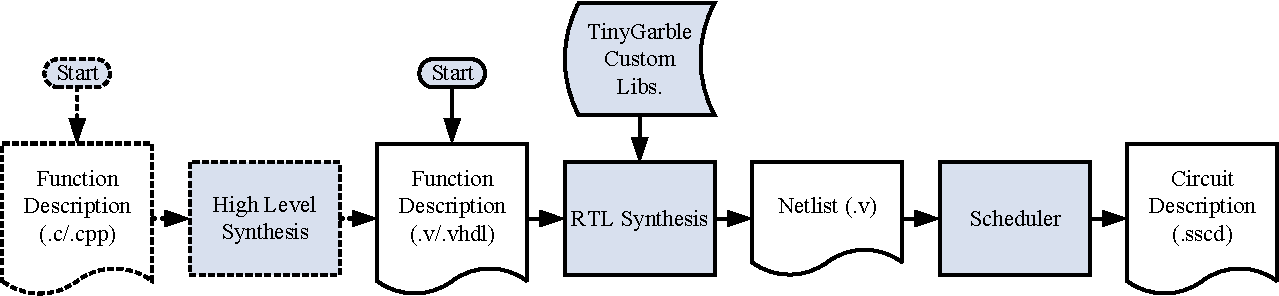
\includegraphics[width=0.95\textwidth]{synthesis_flow-crop.pdf}
\caption{\gls{tinygarble} \acrshort{gc} synthesis flow.
  The inputs can be either a \gls{c}/C++ program (translatable to \acrshort{hdl} via a standard \acrshort{hls} tool) or a direct \acrshort{hdl} description.
  The output is a scheduled circuit description ready to be garbled/evaluated.}
\label{fig:synthesis-flow}
\end{figure}

\begin{enumerate}
\item The input to \gls{tinygarble} \acrshort{gc} synthesis is a file that describes a function written in an \acrshort{hdl} like \gls{verilog} or \gls{vhdl}.
      The function can also be written in a high level language like \gls{c}/C++ and automatically translated to \acrshort{hdl} using an \acrshort{hls} tool.

\item A standard logic synthesis tool compiles the \acrshort{hdl} to generate the netlist file.
      The synthesis tool optimizes the netlist based on the user defined objectives/constraints and customized library.
      The contains and library are set such that the netlist is optimized for evaluation in the \acrshort{gc} protocol.

\item The netlist is parsed and topologically sorted.
      Then, the sorted netlist is stored in format readable by \gls{tinygarble} \acrshort{gc} engine.
\end{enumerate}

\begin{figure}
\centering
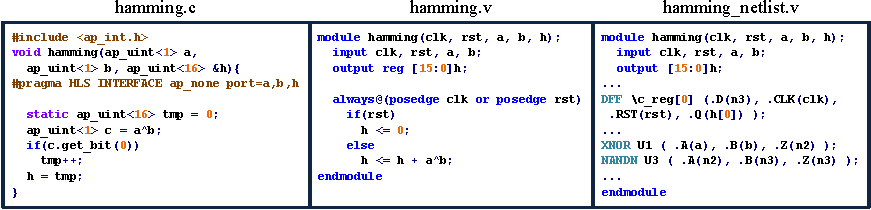
\includegraphics[width=\textwidth]{HLS_HDL_netlist-crop.pdf}
\caption{Sample files at the different steps of \gls{tinygarble} \acrshort{gc} synthesis flow for Hamming distance function.}
\label{fig:globalflow_sample}
\end{figure}

\fig{fig:globalflow_sample} shows examples of files at different steps of \gls{tinygarble} \acrshort{gc} synthesis flow for Hamming distance function.
The \textsl{hamming.c} file contains the description of the function in the \gls{c} language.
The user inputs this function to a \acrshort{hls} tool to generate the corresponding description in \gls{verilog}.
The resulting \gls{verilog} file is functionally similar to the \textsl{hamming.v} file shown in the figure, but it may look more complicated and be less efficient as it is generated by an automated tool.
A user can also write the description directly in \gls{verilog} to have more control on the circuit and therefore a more efficient netlist.
The \textsl{hamming.v} file is provided to a logic synthesis tool along with the \gls{tinygarble} custom libraries to generate netlist \textsl{hamming\_netlist.v}.
The netlist describes the same function as \textsl{hamming.c} and \textsl{hamming.v} but uses the logic cells provided in the technology library.
The technology library contains 2-input-1-output logic cells to be compatible the \acrshort{gc} protocol.

In the following, we describe the details of the synthesis steps and how we manipulate the synthesis tools in each of the steps to generate optimized netlists for the \acrshort{gc} protocol.

\section{Synthesis library}\label{sec:syn-synlib}
The first step in the synthesis flow is to convert arithmetic and conditional operations like add, multiply, and if-else to their logical representations that fits best to the user's constraints.
For example, the sum of two N-bit numbers can be replaced with an N-bit ripple carry adder in case of area optimization or an N-bit carry look ahead adder in case of timing optimization.
A library that consists of these various implementations is called a \emph{synthesis library}.
We develop our own synthesis library that includes implementations customized for the \acrshort{gc} protocol.
In this library, we build the arithmetic operations based on a full adder with one non-XOR gate \cite{boyar2006concrete} and conditional operations based on a 2-to-1 multiplexer (\acrshort{mux}) with one non-XOR gate \cite{kolesnikov2008improved}.

\section{Technology library}\label{sec:syn-techlib}
The next step is to map the structural representation onto a \emph{technology library} to generate the netlist.
A technology library contains basic units available in the target platform.
For example, tools targeting \acrfull{fpga} like Xilinx \acrshort{ise} or Quartus contain Look-Up Tables and Flip Flops in their technology libraries, which form the architecture of an \acrshort{fpga}.
On the other hand, tools targeting \acrfull{asic} like \gls{synopsys-dc}, Cadence, and ABC, may contain a more diverse collection of elements starting from basic gates like AND, OR, etc., to more complex units like \acrshort{ff}s.
The technology library contains logical descriptions of these units along with performance parameters like their delay and area.
The goal of the synthesis tool in this step is to generate a netlist of library components that best fit the given constraints.
For logic synthesis, we use tools targeting \acrshort{asic}s as they allow more flexibility in their input technology library.
We design a custom technology library that contains 2-input gates as they incur minimum garbled tables in the \acrshort{gc} protocol compared to gates with more inputs.
We set the area of XOR gates to 0 and the area of non-XOR gates to a non-0 value, e.g., 1.
By choosing area minimization as the only optimization goal, the synthesis tool produces a netlist with the minimum possible number of non-XOR gates.
This reduces the total computation and communication of the \acrshort{gc} protocol due to the Free XOR optimization \cite{kolesnikov2008improved}.

An additional feature of our custom technology library is that it contains non-standard gates (other than basic gates like NOT, AND, NAND, OR, NOR, XOR, and XNOR) to increase flexibility of mapping process.
For example, the logical functions $F = A\wedge B$ and $F = (\neg A)\wedge B$ requires equal effort in garbling/evaluation.
However by using only standard gates, the second function will require two gates (a NOT gate and an AND gate) and store one extra pair of labels for $\neg A$ in the memory.
We include four such non-standard gates with an inverted input in our custom library.
XOR, XNOR, and NOT gates are free so their area is set to 0.
The area of the rest of gates, similar to the area of non-XOR, is set 1.
In order to be consist with the previous work in the literature, we use ``number of non-XOR gates'' to refer to the number of non-free gates in a circuit throughout this thesis.
Due to the Free XOR optimization, this metric directly corresponds to time and communication cost of garbling/evaluating the circuit.

\section{Offline Circuit Synthesis}\label{sec:syn-offline}
In \gls{tinygarble} \acrshort{gc} synthesis, we use logic synthesis tools in an offline manner to generate a circuit for a given functionality.
This offline synthesis followed by a topological sort provides a ready-to-use circuit description for any \acrshort{gc} implementations including our \gls{tinygarble} \acrshort{gc} engine.
This approach, unlike online circuit generation, does not require misspending time for circuit generation during garbling/evaluation.
It also enables the use of beneficial synthesis optimization techniques that were previously infeasible for online generation.
Moreover, the synthesis tools have a global view of the circuit, unlike previous work that manually optimized small modules of the circuit.
This allows more effective optimization for any arbitrary function and set of constraints.

\section{Limitation}\label{sec:syn-limit}
The synthesis approach has certain limitations when it comes to generating combinational circuits for extremely large functions.
The amount of memory and computation resources required by logic synthesis tools considerably increase for generating large combinational circuits.
Generally, synthesis tools are not designed to support such large scale combination circuits.
This means logic synthesis for \acrshort{gc} cannot be scaled, at least automatically, for large functions using current setting, i.e., synthesizing its combinational circuit.

However, most of these large functions include one or more recurring computation blocks (a.k.a, loops).
In combinational representation, these loops have to be unfolded and represented as repeated blocks in the circuits.
In hardware design, these functions are folded around their loops and are described using sequential circuits.
A sequential circuit has feedback loops and is evaluated for multiple times (sequential cycles), thus it is the most suited to represent the recurring blocks in large functions.
In the next chapter, we will discuss possibility of using sequential circuit for the \acrshort{gc} protocol.
We will show how can we exploit loops in sequential circuits while the process of optimized circuit generation remains the same.
This allows us to befit from synthesis tools optimization even for large functions.

% !TEX root = 0_main.tex
\chapter{Sequential Garbled Circuits}\label{chap:seq}
Sequential circuits can be used as a very compact Boolean circuit description. We use sequential description to overcome the scalability limitation of the synthesis approach for combinational circuits.
In the following chapter, we first describe the concept of sequential circuits using an example.
Next, we discuss synthesizing sequential circuit for the \acrshort{gc} protocol.
Then, we explain the modifications required to garble/evaluate sequential circuits.

\section{Sequential Circuits}\label{sec:seq-seq}
In the context of the \acrshort{gc} protocol, we can defined sequential circuit as a folded version of combinational circuit that needs to be evaluated multiple cycle.
Unlike combinational circuits where the output depends only on the inputs, the output of sequential circuit depends on both input and the state of the circuit stored in its memory.
Usually, intermediate values during computation is stored as a state of the circuit and is used in later cycles to complete computation of the function.
In following, we illustrate the difference between combination and sequential circuit using a simple 4-bit adder as a function.

\begin{figure}[ht]
    \centering
    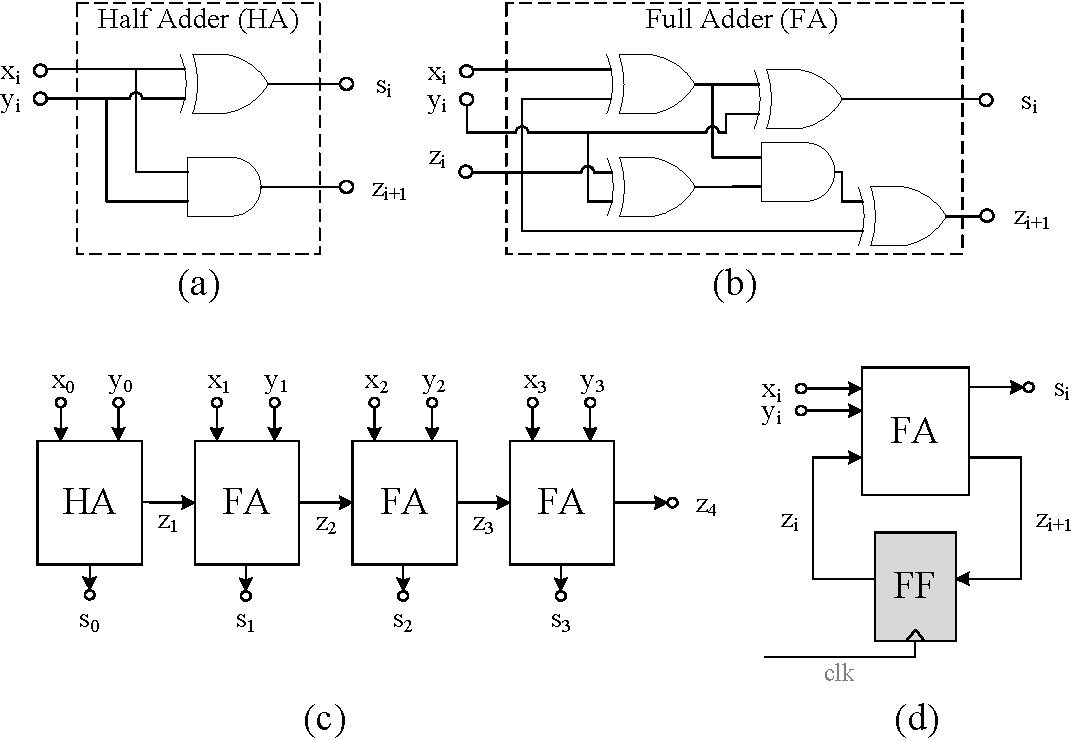
\includegraphics[width=0.7\textwidth]{adder-crop.pdf}
    \caption{Combinational and sequential design of a 4-bit Adder.
  (a) HA circuit.
  (b) FA circuit.
  (c) Combinational 4-bit Adder using 1 HA and 3 FAs.
  (d) Sequential 4-bit Adder using one FA.}\label{fig:combSeq}
\end{figure}

\fig{fig:combSeq} demonstrates an example of a combinational and a sequential implementation for a 4-bit Adder function with inputs $x = \overline{x_3x_2x_1x_0}$ and $y = \overline{y_3y_2y_1y_0}$, producing sum $s = \overline{s_3s_2s_1s_0} = f(x, y) = x + y$.
\fig{fig:combSeq}a and \ref{fig:combSeq}b show the internal combinational circuit of a half Adder (HA) and a full Adder (FA) respectively.
In \fig{fig:combSeq}c a combinational Adder is built by cascading 3 FAs and one HA.
\fig{fig:combSeq}d represents a sequential implementation of a 4-bit Adder which uses one FA and a one bit \acrshort{ff} to save the carry bit from the previous cycle.
The circuit should be evaluated for 4 cycles.
At the first cycle the carry bit is $z_0=0$.
Note that, in the combinational circuit we use three FAs and one HA whereas in the sequential circuit, we have to use one FA for 4 sequential cycles.
This asymmetry in the loop of Addition function introduces a small \emph{overhead} in \acrshort{gc} computation and communication time as an HA circuit has fewer gates compared to a FA circuit.
We will discuss the overhead of garbling sequential circuits and its sources in more detail in \sect{sec:seq-overhead}.

However, the total number of gates for representing the function is reduced approximately by a factor of 4 when using a sequential circuit (one FA for sequential compared with three FA and one HA for combinational).
This helps to limit the memory footprint for garbling and evaluation required for storing circuit description and wire labels ($k$-bit per wire, see \sect{ssec:prelim-gc}).
In a sequential circuit, the number of labels that need to be stored in memory at any moment is proportional to the number of gates in the circuit.
The wire labels are simply over-written at each sequential cycle.
Only labels corresponding to FFs are kept for the next cycle.

Nearly all commercial circuits used in digital hardware are designed in sequential format.
There are multiple reasons for preferring sequential circuit description over combinational including the reduction in complexity, area, power, and cost, as well as natural mapping of finite state machine control functions into a sequential format.
Some of these reasons also provide a rationale for sequential description of a function in \acrshort{gc}, including: (i) reduction in size and memory footprint that is achieved by introducing the state elements and feedback loop from output to input; (ii) removing the need to perform costly compile-time/runtime loop unrolling by embracing loops within the sequential feedback loop; (iii) providing a new degree of freedom for folding by the placement of memory elements in the long combinational paths--the placement can be done in accordance with the user's objective; (iv) solving the limitation of synthesis techniques and tools for large function (see /sec{sect:syn-limit}) by describing circuits in compact sequential format.

\begin{figure}[ht]
  \centering
  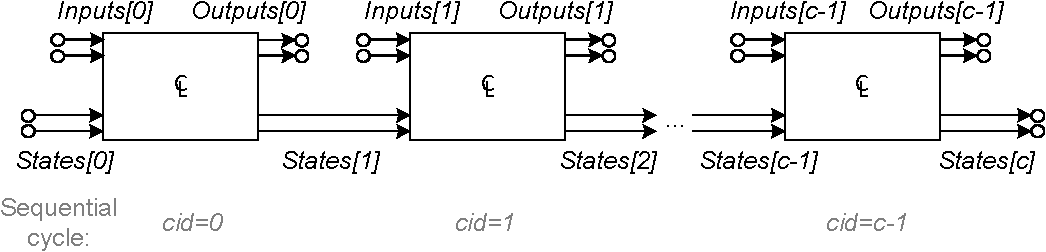
\includegraphics[width=0.8\textwidth]{sequential-open-crop.pdf}
  \caption{Functionally equivalent unrolled sequential circuit corresponding to \fig{fig:sequential}.}
  \label{fig:open-sequential}
\end{figure}

During the evaluation of a sequential circuit, the combinational block is evaluated $c$ times where $c$ is the number of sequential cycles that the circuit operates.
We can visualize this process as the unrolled combinational representation of the sequential circuit as shown in \fig{fig:open-sequential}.
$c$ also shows the folding factor of the sequential circuit ($c=1$ means the circuit is combinational).
The inputs/outputs of the unrolled circuit are the inputs/outputs of the combinational block in all the cycles.
The present states at each cycle $\textrm{cid}$, where $0 \le \textrm{cid} < c$, are equal to the next states at the previous cycle ($\textrm{cid}-1$).
The present states at $\textrm{cid}=0$ are equal to the input initial value.

In digital hardware, at edge of a cycle, the value of D of an \acrshort{ff} is latched and then transfered to the Q in the next clock cycle.
In garbling/evaluating of a sequential circuit, an \acrshort{ff} operates as a simple wire connection between the the unrolled combinational circuit in two consecutive cycles.
Thus, it can be dealt with latching the labels from the flip-Flop input D in $\textrm{cid}$ to output Q in $\textrm{cid}+1$.
Signal clk and rst of \acrshort{ff} can be ignored in sequential \acrshort{gc}.

Garbling/evaluation of the sequential circuit is equivalent of garbling its gates for $c$ times.
To make sure that the security and correctness of the \acrshort{gc} protocol still holds for the sequential circuits, we use combination of cycle index and gate identifier for the the encryption tweak $T$ (see \sect{sssec:prelim-aes}).
This way a unique tweak is assigned for the same gates in different cycles makes it same as garbling a unrolled combinational circuit.

In \appx{chap:engine}, we discuss our implementation of the \acrshort{gc} protocol for sequential circuits in TinyGarble \acrshort{gc} engine.
We also explain in more detail about how the encryption tweak is set and how it affects the security and correctness of the \acrshort{gc} protocol.

\section{Synthesis Sequential Circuit}\label{sec:seq-syn}
Fortunately, extending TinyGarble \acrshort{gc} synthesis to support sequential circuits is straightforward since the synthesis tools are designed to work them in the first place.
We add memory element of sequential circuits into the technology library of TinyGarble (see \sect{sec:syn-techlib}).
These elements can be implemented as FFs which are connected to a clock signal.
Although in conventional ASIC design FFs are typically as costly as four NAND gates, as seen above in our \acrshort{gc} application, FFs do not have any impact on the garbling/evaluation process as they require no cryptographic operations.
Therefore, we set the area of FFs to 0 to show its lack of impact on computation and communication time of garbling/evaluation.
Moreover, we modify our FFs such that they can accept an initial value.
This helps us remove extra MUXs in standard \acrshort{ff} design for initialization.

Describing functions using sequential circuits helps to overcome the scalability limitations of synthesis tool.
Sequential circuits are radically smaller than combinational ones with the same functionality.
This property allows synthesis tools to not only generates the circuit with less recourses, but to find a more optimized circuit.
Moreover, the compatibility of our sequential descriptions with standard synthesis tools simplifies the workflow of circuit generation for \acrshort{sfe} applications.

\section{Overhead of Sequential Circuit}\label{sec:seq-overhead}
In sequential circuit, the function is divided into smaller steps such that one step is computed at each cycle.
If a function can be divided into identical steps, only one step is implemented in the sequential circuit.
Evaluating the sequential circuit for multiple cycles ensures that the function is computed completely.
However, many functions does not have such symmetrical structure and cannot be divided perfectly into identical steps.
The sequential circuit of such a function includes different sub-circuits that each corresponds to one of the steps in the function.

\fig{fig:seq-overhead-comb} shows an example of such function that is represented as a combinational circuit.
The computation in the function can be divided into 6 non-identical steps.
The computation in the first and last steps are different from the rest.
U1 sub-circuit represents the computation in the first step, U2 the middle four steps, and U3 the last step.
\fig{fig:seq-overhead-seq} illustrates the sequential circuit representation of the example function.
A \acrshort{mux} selects the output of the sub-circuits according to the cycle id (cid).
In the digital circuit design, \acrshort{mux} and similar components that control the flow of data is called control path.
If cid is 0, U1 is selected, if it is 5, U3 is selected, otherwise U2 is selected.
The unselected sub-circuits remain idle in that cycle, since its output is not used.
At each cycle, the output of the selected sub-circuit is stored in the \acrshort{ff} to be used in the next cycles.

\begin{figure}[ht]
    \centering
    \begin{subfigure}[t]{0.8\textwidth}
        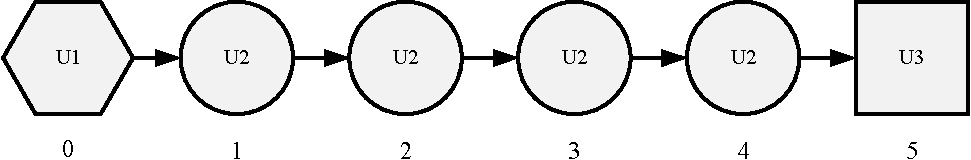
\includegraphics[width=\textwidth]{seq-overhead-comb-crop.pdf}
        \caption{Combination Circuit.}\label{fig:seq-overhead-comb}
    \end{subfigure}
    \begin{subfigure}[t]{0.7\textwidth}
        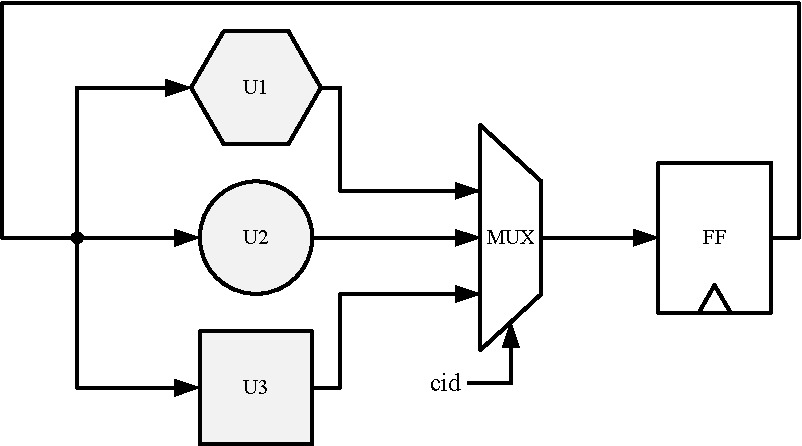
\includegraphics[width=\textwidth]{seq-overhead-seq-crop.pdf}
        \caption{Sequential Circuit.}\label{fig:seq-overhead-seq}
    \end{subfigure}\\
    \caption{The combinational and sequential representations of a function with an asymmetric structure.
    The sequential implementation has to be evaluated for 6 cycles and eventually needs more gates to be garbled/evaluated compared to the combinational one.}\label{fig:fig:seq-overhead-comb}
\end{figure}

The number of gates that has to garbled/evaluated in the combinational circuit is $C_{U1}+4*C_{U2}+C_{U3}$, where $C_{Ui}$ is the number of gates in $Ui$ sub-circuit.
Since the sequential circuit has to be garbled/evaluated for 6 times, the total gates for sequential circuit is $6*(C_{U1}+C_{U2}+C_{U3}+C_{\acrshort{mux}})$, where $C_{\acrshort{mux}}$ is number of non-XOR in the \acrshort{mux}.
The difference between the cost of the combinational and the sequential circuits is $5*C_{U1}+2*C_{U1}+5*C_{U3}+6*C_{\acrshort{mux}})$.
We call this difference the sequential \textit{overhead} for garbling an asymmetrical function.

The overhead is caused by treating cid as a secret value in the \acrshort{gc} protocol while both parties known its value at all cycles.
In the next chapter, we will discuss how to reduce this overhead using a novel algorithm on top of sequential \acrshort{gc} protocol.
The algorithm skips unnecessary garbling/evaluation of idle sub-circuits and allows local computation of the gates in the control path.

% !TEX root = 0_main.tex
\chapter{{\gls{skipgate}}: Reducing Sequential Overhead}\label{chap:skipgate}
\gls{skipgate} is developed to work with the \acrshort{gc} protocol to reduce the overhead of sequential circuits.
It allows secure evaluation of functions in the form of $c = f(a, b, p)$ where $p$ is the public input known to both parties and $a$ and $b$ are the private inputs.
The goal of \gls{skipgate} is to reduce the circuit of $f(a, b, p)$ into a simpler circuit of $c = f_p(a,b)$ with the same logic for a given public input $p$.
Secure evaluation of $f_p(a,b)$ costs less than that of $f(a, b, p)$ using the conventional \acrshort{gc} protocol where $p$ is treated as a private input.
For doing so, \gls{skipgate} removes communication cost of garbling for a gate when its output can either be computed independently by Alice and Bob or has no effect on the final output.
In other words, \gls{skipgate} reduces the communication between the parties when it can be replaced by less costly local computation.
The cost reduction is especially significant in a sequential circuit where the control path is public and independent of the private inputs.

In this chapter, first we introduce the notation used in \gls{skipgate} algorithm.
Next, a motivational example is provided to present the sequential overhead.
Next, We discuss how gates in a circuit are categorization in \gls{skipgate}.
The pseudo-code of the \gls{skipgate} algorithm is then provided with its complexity analysis and correctness and security proofs.

\section{Notations}\label{sec:skipgate-notation}
In a classic Boolean circuit, each wire $w$ carries a value ($x_w\in\{0, 1\}$), whereas in a garbled circuit, each wire carries a pair of labels ($X_w^{0}$ and $X_w^{1}$) on Alice's side and one label ($X_w \in \{X_w^{0}, X_w^{1}\}$) on Bob's.
If $X_w = X_w^{0}$, the actual Boolean value is 0 and if $X_w = X_w^{1}$, it is 1.
This means that the information is shared between two parties.
In our scheme, we combine these notions of Boolean and garbled circuits.
Each wire either carries a Boolean value known to both parties independently (\textit{public} wire) or it carries a (pair of) label(s) (\textit{secret} wire).

\section{Motivational Example}\label{sec:skipgate-motiv}
\fig{fig:mux} illustrates a sequential circuit that has a control path with a 2-to-1 \acrshort{mux} whose inputs come from two sub-circuits f$_0$ and f$_1$ connecting to \acrshort{mux} input 0 and 1 respectively.
At a certain clock cycle, if the select wire of the \acrshort{mux} ($x$) is public, say equal to 1, both parties know that the gates in the sub-circuit f$_0$ do not need to be garbled/evaluated since they have no effect on the final output.
The gates in the \acrshort{mux} itself act as wires and pass the output of f$_1$ to the \acrshort{mux} output, thus the gates in the control path do not need to be garbled/evaluated in that clock cycle either.
However in the conventional \acrshort{gc} protocol where public wire $x$ was teared as a secret value, the entire circuit had to be garbled/evaluated.
In the following subsection, we explain how the \gls{skipgate} algorithm identifies such gates to reduce the garbling cost in circuits with public wires.

\begin{figure}[h]
    \centering
    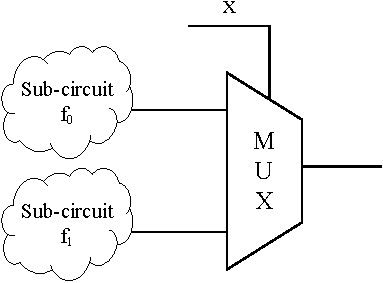
\includegraphics[width = 0.45\textwidth]{mux-crop.pdf}
    \caption{Motivational example: two sub-circuits connecting to a \acrshort{mux} with a public select signal.}
\label{fig:mux}
\end{figure}

It is worth noting that in a sequential garbled circuit presented in \chap{cahp:seq}, the Boolean value of a wire can change at every clock cycle.
A wire may also alter between being secret and public.
The \gls{skipgate} algorithm is executed once for each sequential cycle.
\gls{skipgate}'s decision on each gate (locally computing, garbling/evaluating, or skipping) depends on the status of the gate's inputs (public or secret) on that cycle.
Thus, \gls{skipgate} is fundamentally different compared to offline circuit simplification methods such as the one introduced in~\cite{pinkas2009secure} which remove gates with known constant inputs.
The constant gates are already removed in our circuits that are generated by the conventional \acrshort{hdl} synthesis tools.

\section{Gate Categories}\label{sec:skipgate-cat}
The \gls{skipgate} algorithm classifies the gates into four categories in terms of the parties' knowledge about their inputs:

\begin{enumerate}[label=\roman*]
  \item \textit{Gate with two public inputs.}
    In this case, the output is public.
  \item \textit{Gate with one public input.}
  	Depending on the gate type, the output becomes either public or secret.
  	For example, for an AND gate with 0 at one input, the output becomes 0.
  	This means that if the secret input is not connected to any other gate, the gate generating it can be skipped for garbling/evaluation.
  	If the public input is 1, then the AND gate acts as a wire and the output wire carries the label of the secret input.
  \item \textit{Gate with secret inputs that have identical (or swapped) labels.}
    This indicates that the two secret inputs have identical (or inverted) Boolean values.
    (We will explain shortly how Bob identifies the swapped case.)
    Depending on the gate type, the output becomes either public or secret.
    For example, the output of an XOR gate with two inverted inputs (either secret or public) is always 1 (public).
  	Similar to Category ii, the gate generating the inputs, if not connected to any other gates, can be skipped for garbling/evaluation.
  \item \textit{Gate with unrelated secret inputs.}
  	The output is always secret.
  	The gate has to be garbled/evaluated conventionally according to the \acrshort{gc} protocol.
    However, if its output does not have any effect on the circuit output, the gate is skipped, i.e., the corresponding garbled table is not transfered from Alice to Bob.
\end{enumerate}

\section{Algorithm}\label{sec:skipgate-alg}

\begin{algorithm}[]
\caption{\gls{skipgate}, Alice's side.}\label{alg:alice}
\textbf{Inputs:} Sequential \texttt{circuit} of $f(a,b,p)$, Alice's input $a$, public input $p$, number of clock cycles $cc$.\\
\textbf{Outputs:} Pairs of output labels $X^0_c$ and $X^1_c$.\\
\begin{algorithmic}[1]
\STATE{\bf{SkipGate\_alice\ (circuit, a, p, cc)}:}
\STATE{($X^0_a,X^1_a,X^0_b,X^1_a$) = generate\_random\_labels()}
\STATE{send\_alice\_labels($a, X^0_a, X^1_a$)}
\STATE{send\_bob\_labels($X^0_b, X^1_b$) \textit{ // through \acrshort{ot}}}
\STATE{circuit.set\_private\_input($X^0_a,X^1_a,X^0_b,X^1_a$)}
\STATE{circuit.set\_public\_input($p$)}
\FOR{cid in [$0 ... cc-1$]}
  \STATE{circuit.initial\_label\_fanout()}
  \STATE{circuit.phase1()}
  \STATE{garbled\_tables = circuit.phase2\_alice()}
  \STATE{send\_garbled\_tables(garbled\_tables)}
  \STATE{circuit.transfer\_flip\_flops\_labels()}
\ENDFOR
\STATE{($X^0_c,X^1_c$) = circuit.get\_output\_label()}
\STATE{$X_c$ = receive\_bob\_output\_label()}
\STATE{$c$=get\_output\_value($X^0_c,X^1_c,X_c$)}
\end{algorithmic}
\end{algorithm}

\begin{algorithm}[]
\caption{\gls{skipgate}, Bob's side.}\label{alg:bob}
\textbf{Inputs:} Sequential \texttt{circuit} of $f(a,b,p)$, Bob's input $b$, public input $p$, number of clock cycles $cc$.\\
\textbf{Outputs:} Output label $X_c$.\\
\begin{algorithmic}[1]
\STATE{\bf{SkipGate\_bob(circuit, b, p, cc)}:}
\STATE{$X_a$ = receive\_alice\_labels()}
\STATE{$X_b$ = receive\_bob\_labels($b$) \textit{//through \acrshort{ot}}}
\STATE{circuit.set\_private\_input($X_a,X_b$)}
\STATE{circuit.set\_public\_input($p$)}
\FOR{cid in [$0 ... cc-1$]}
  \STATE{circuit.initial\_label\_fanout()}
  \STATE{circuit.phase1()}
  \STATE{garbled\_tables = receive\_garbled\_tables()}
  \STATE{circuit.phase2\_bob(garbled\_tables)}
  \STATE{circuit.transfer\_flip\_flops\_labels()}
\ENDFOR
\STATE{$X_c$ = circuit.get\_output\_label()}
\STATE{send\_output\_label($X_c$)}% \textit{//send the output label to Alice}
\end{algorithmic}
\end{algorithm}

\alg{alg:alice} and \alg{alg:bob} show the \gls{skipgate} algorithm for Alice and Bob sides respectively.
Lines 2-5 of \alg{alg:alice} and Lines 2-4 of \alg{alg:bob} are similar to the \acrshort{gc} protocol label generation and transfer for both sides.
The \gls{skipgate} algorithm has two main phases:
In Phase 1, the outputs of the gates with public input (Categories i-ii) are computed.
In Phase 2, the gates with private inputs (Categories iii-iv) are  garbled/evaluated.
For each round of sequential cycle, Alice executes Phase 1 and 2 of \gls{skipgate} and sends the generated garbled tables to Bob.
Bob receives the tables and executes two phases in order to evaluate the gates.
In Line 12 of \alg{alg:alice} and Line 11 of \alg{alg:bob}, the labels associated to the input of flip-flops are transfered to their output for the next cycles as required by sequential \acrshort{gc} protocol (see \sect{sec:seq-seq}).
Similar to conventional \acrshort{gc}, at the end, Alice learns pairs of labels for each output wire and Bob has one of the pairs; they share this information to learn the output $c$.
For example, in the case where Alice intends to learn the final output, she receives the Bob's output label and together with her input labels finds the real output value (Line 15-16 of \alg{alg:alice} and Line 14 of \alg{alg:bob}).

In \gls{skipgate}, an integer called \texttt{label\_fanout} is associated with each gate and indicates the number of times the gate's output label is used (either as a circuit's output or an input to other gates).
At the beginning of each cycle (Line 8 of \alg{alg:alice} and \alg{alg:bob}), the \texttt{label\_fanout} is set to the gate fanout in the circuit\footnote{\textit{Fanout} of a gate, borrowed from hardware design, is the number of subsequent gates (and circuit outputs) dependent on the gate’s output.}.
\texttt{label\_fanout} of a gate may decrease if its output label is not needed anymore, e.g., a gate whose output is connected an AND gate with 0 at the other input (Category ii).
If \texttt{label\_fanout} reaches 0, it means that gate's output label does not have any effect on the final output.
The gates with \texttt{label\_fanout}=0 are subsequently designated for skipping, which in turn decreases the \texttt{label\_fanout} of their input gates recursively.
Finally, the gates in Category iv that have not been marked for skipping are garbled/evaluated.

\begin{algorithm}[]
\caption{Phase 1 in \gls{skipgate} for both Alice and Bob sides.}\label{alg:phase1}
\begin{algorithmic}[1]
\STATE{\bf{circuit.phase1()}:}
\FOR{g in circuit}
	\IF{g.i0 is public and g.i1 is public \textit{//Category i}}
		\STATE{g.o = public\_calculate(g.type, g.i0, g.i1)}
		\STATE{g.label\_fanout $= 0$}
	\ELSIF{g.i0 is public or g.i1 is public \textit{//Category ii}}
		\STATE{g.o = g.half\_public\_calculate(g.type, g.i0, g.i1)}
		\IF{g.o is public}
			\STATE{g.label\_fanout $= 1$ \textit{//will become zero in recursive\_reduction()}}
			\STATE{circuit.recursive\_reduction(g)}
		\ENDIF
	\ENDIF
\ENDFOR
\end{algorithmic}
\end{algorithm}

\alg{alg:phase1} illustrates Phase 1 of \gls{skipgate} in which Alice and Bob find and compute the gates that belong to Categories i-ii.
\texttt{label\_fanout}s of the gates in Category i are set to zero.
For gates in Category ii, if the output becomes public, \gls{skipgate} decreases the \texttt{label\_fanout} of the secret input's originating gates recursively by invoking \texttt{recursive\_reduction} (\alg{alg:skipgate_reduction}).
\fig{fig:phaseOneExample} shows four different examples in Phase 1.

Bob does not receive any information from Alice about the gates in Category i-ii because he can locally evaluate Phase 1 just like Alice.
An alternative approach is that Alice sends the result of Phase 1 to Bob.
This approach has two main disadvantageous:
First, it makes the protocol complicated if one wants to enhance the security of the protocol to be secure against malicious adversaries.
Second, it increases the communication overhead which is the bottleneck of the \acrshort{gc} protocol.

\begin{figure}[h]
    \centering
    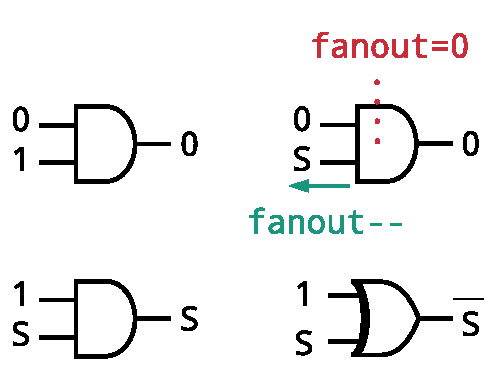
\includegraphics[width=0.40\textwidth]{phaseOneExample-crop.pdf}
    \caption{Four examples of replacing gates in Phase 1 by zero, one, wire, or inverter.
    \texttt{label\_fanout} is decreased for the unnecessary gate.
    The top-left example is in Category i and the rest are in Category ii.}
    \label{fig:phaseOneExample}
\end{figure}

\begin{algorithm}[]
\caption{Phase 2 in \gls{skipgate}, Alice's side.}\label{alg:phase2_alice}
\textbf{Output}: \texttt{garbled\_tables} queue.\\
\begin{algorithmic}[1]
\STATE{\bf{circuit.phase2\_alice()}:}
\FOR{g in circuit where g.label\_fanout $> 0$}
	\IF{(g.i0.label is equal g.i1.label or\\
		g.i0.label is inverted g.i1.label) \textit{//Category iii}}
		\STATE{g.o = related\_secret\_calculate(g.type, g.i0, g.i1)}
		\IF{g.o is public}
			\STATE{g.label\_fanout $= 1$ \textit{//will become zero in recursive\_reduction()}}
			\STATE{circuit.recursive\_reduction(g)}
		\ENDIF
	\ELSE \STATE{\textit{//Category iv}}
    \STATE{(g.o, g.table) = garble(g.type, g.i0, g.i1) \textit{//table=null for XOR}}
    \IF{g is non-XOR}
      \STATE{garbled\_tables.enqueue(g.id, g.table)}
    \ENDIF
	\ENDIF
\ENDFOR
\STATE{garbled\_tables.filter(t : circuit[t.id].label\_fanout $> 0$)}
\end{algorithmic}
\end{algorithm}

\alg{alg:phase2_alice} shows the Phase 2 of \gls{skipgate} for Alice's side in which she performs the same task for Category iii.
She then generates garbled tables for gates with non-zero \texttt{label\_fanout} in Category iv.
\fig{fig:phaseTwoExample} shows four different examples in this phase.
By the end of Phase 2, due to the recursive nature of the fanout reduction, \texttt{label\_fanout} of some gates that have already been garbled may become 0.
In Line 17 of \alg{alg:phase2_alice}, Alice filters the garbled tables that have non-zero \texttt{label\_fanout} to be sent to Bob.

\begin{figure}[h]
    \centering
    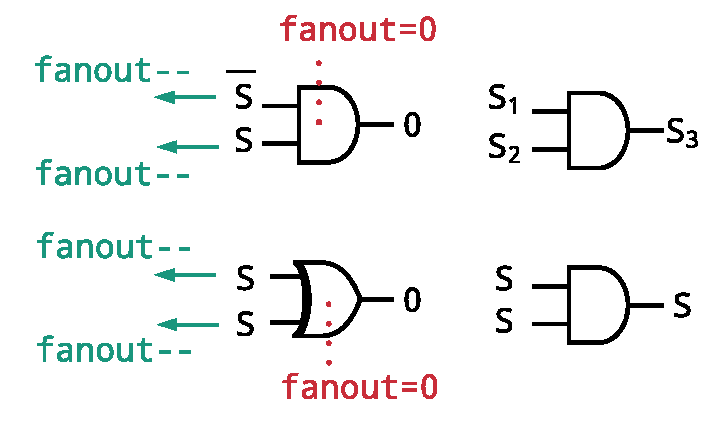
\includegraphics[width = 0.50\textwidth]{phaseTwoExample-crop.pdf}
    \caption{Four examples of replacing and computing gates in Phase 2.
    		 \texttt{label\_fanout} is decreased for the unnecessary gates.
         The top-right example is in Category iv, and the rest are in Category iii.}
    \label{fig:phaseTwoExample}
\end{figure}

\begin{algorithm}[]
\caption{Phase 2 in \gls{skipgate}, Bob's side.}\label{alg:phase2_bob}
\textbf{Input}: \texttt{garbled\_tables} queue.\\
\begin{algorithmic}[1]
\STATE{\bf{circuit.phase2\_bob(garbled\_tables)}:}
\FOR{g in circuit where g.label\_fanout $> 0$}
	\IF{(g.i0.label is equal g.i1.label or\\
		g.i0.label is inverted g.i1.label) \textit{//Category iii}}
		\STATE{g.o = related\_secret\_calculate(g.type, g.i0, g.i1)}
		\IF{g.o is public}
			\STATE{g.label\_fanout $= 1$ \textit{//will become zero in recursive\_reduction()}}
			\STATE{circuit.recursive\_reduction(g)}
		\ENDIF
	\ELSE \STATE{\textit{//Category iv}}
    \IF{g is XOR}
     \STATE{g.o = g.eval\_XOR(g.i0, g.i1)}
    \ELSIF{g.id is garbled\_tables.top().id}
      \STATE{gt = garbled\_tables.dequeue().table}
      \STATE{g.o = g.eval(g.type, g.type, g.i0, g.i1, gt)}
    \ELSE
      \STATE{g.o = next\_unique\_label() \textit{//generate a unique label.}}
    \ENDIF
	\ENDIF
\ENDFOR
\end{algorithmic}
\end{algorithm}

\alg{alg:phase2_bob} shows the Phase 2 for Bob's side.
Bob evaluates the gates that belong to Category iii and iv.
In Line 17 of \alg{alg:phase2_bob}, Bob generates and assigns new unique labels (\texttt{next\_unique\_label}) for gates that were filtered by Alice.
Bob knows that the \texttt{label\_fanout} of these gates will eventually become 0.
Therefore, he produces new labels for them only to keep track of these secret variables that are used to compute the output of the gates in Category iii.
He can generate these labels randomly or use a monotonic counter that increase by one for each newly generated label.
To distinguish valid \acrshort{gc} labels from his generated labels, he keeps a single bit flag beside each label that indicates the label is generated by him and is not valid for \acrshort{gc} evaluation.

\begin{algorithm}[]
\caption{Recursive Fanout Reduction of \gls{skipgate}.}\label{alg:skipgate_reduction}
\textbf{Inputs:} Gate \texttt{g} (where the reduction starts).\\
\begin{algorithmic}[1]
\STATE{\bf{circuit.recursive\_reduction(g)}:}
\IF{g.label\_fanout is  0}
	\STATE{return}
\ENDIF
\STATE{g.label\_fanout = g.label\_fanout - 1}
\IF{g.label\_fanout is  0}
	\IF{g.i0 is secret}
		\STATE{circuit.recursive\_reduction(circuit[g.i0])}
	\ENDIF
	\IF{g.i1 is secret}
		\STATE{circuit.recursive\_reduction(circuit[g.i1])}
	\ENDIF
\ENDIF
\end{algorithmic}
\end{algorithm}


\alg{alg:skipgate_reduction} illustrates the pseudo-code for the recursive fanout reduction.
It receives the circuit and a gate inside the circuit.
It first decreases the \texttt{label\_fanout} of the given gate.
If the \texttt{label\_fanout} becomes 0, it recursively calls itself with the gates that generate the secret input(s).
This process is illustrated on an example circuit in \fig{fig:phaseOneRecursive}.

\begin{figure}[h]
    \centering
    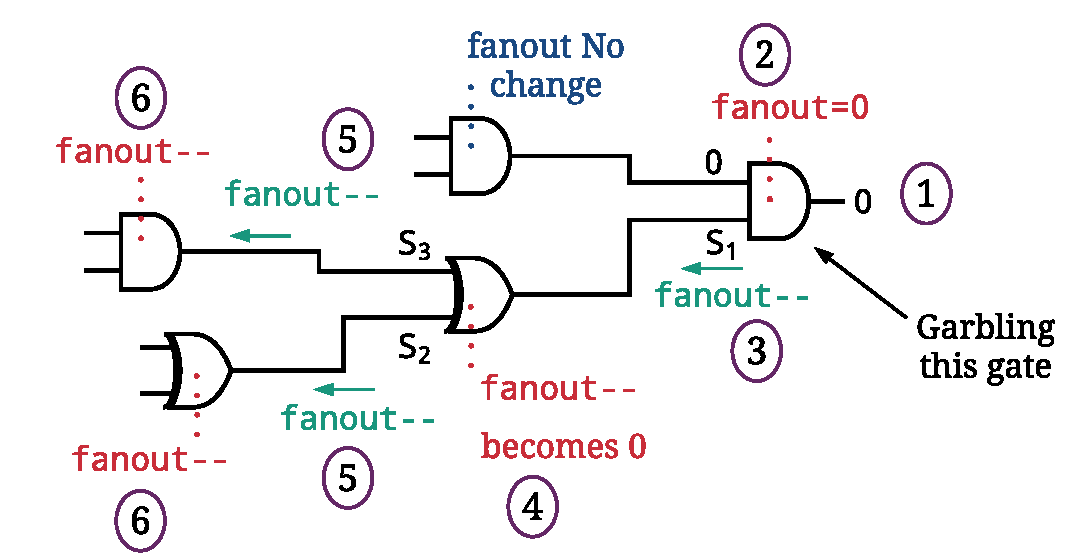
\includegraphics[width=0.8\textwidth]{phaseOneRecursiveExample-crop.pdf}
    \caption{Recursive reduction of \texttt{label\_fanout} to skip unnecessary gates in Phase 1.}
    \label{fig:phaseOneRecursive}
\end{figure}

\subsection{Identification of Identical and Inverted Labels}\label{ssec:skipgate-ident}
According to the \acrshort{gc} protocol, Bob receives only one label $X_w$ for each secret wire $w$.
Due to Free XOR~\cite{kolesnikov2008improved}, he does not need to do anything with a label when it passes a NOT gate because the label's associated with Boolean value is flipped by Alice.
Thus, he cannot tell apart an identical and inverted secret values just by storing labels.
However, it is still possible for Bob to keep track of the flips by storing one bit along with the label.
After evaluating a NOT gate, he simply flips the bit.
The extra bit helps him to differentiate between identical and inverted secret values which is crucial for Phase 2.

\fig{fig:mux_annotated} illustrates the effect of \gls{skipgate} on the example in \fig{fig:mux}.
The gates in the sub-circuit f$_0$ will all be skipped for garbling because their \texttt{label\_fanout} will be zero.
The gates in the \acrshort{mux} also will be bypassed since they belong to Groups (i-iii).

\begin{figure}[h]
    \centering
    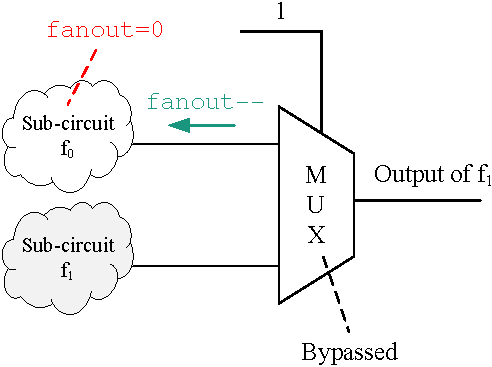
\includegraphics[width = 0.5\textwidth]{mux_annotated-crop.pdf}
    \caption{\gls{skipgate} macro effect on the example in \fig{fig:mux}.
    		 Only sub-circuit f$_1$ is garbled/evaluated.}
\label{fig:mux_annotated}
\end{figure}

\section{Computational Complexity}\label{sec:skipgate-complex}
The \gls{skipgate} algorithm decreases the communication cost of \acrshort{gc}, at the expense of increasing the local computations.
The conventional \acrshort{gc} protocol has a linear computational complexity in terms of the number of gates in the circuit for each sequential cycle.
We show that, despite its recursive appearance, the \gls{skipgate} algorithm does not increase the computation complexity of the \acrshort{gc} protocol.
All parts of the \gls{skipgate} algorithm, except \textit{recursive\_reduction} procedure (\alg{alg:skipgate_reduction}), is executed once per gate, thus they incur a complexity similar to the classic \acrshort{gc} protocol.
The only possible source of complexity increase is \textit{recursive\_reduction} function whose number of invocations depends on the underlying circuit and whether input wires are secret or public.
To find the complexity of \gls{skipgate}, we compute an upper bound on number of invocations of \textit{recursive\_reduction} function.

The termination condition in \textit{recursive\_reduction} is the fanout reaching zero (Lines 2 and 6 of \alg{alg:skipgate_reduction}).
Thus, the worst case scenario is when the function reduces the fanout of all the gates to zero.
In this case, the number of execution of the fanout decrement (Line 5) should be at most the sum of all the initialized fanouts.
\textit{label\_fanout} is initialized with the gate fanout in the circuit.
The upper bound on the sum of fanouts of all the gates in the circuit is $$F = \sum_{i=1}^{n} g[i].fanout \le 2n - m + q,$$ where $n$ is number of gates, $q$ is number of circuit output, and $m$ is number of circuit inputs.
Each gate has two inputs and each input creates a fanout in previous gates unless it is a circuit input.
Also, each output wire incurs the fanout of one.
Both $q$ and $m$ are typically less than or at most in the order of $n$.
Thus, $F$ and subsequently the number of invocation of \texttt{recursive\_reduction} function are $\BigO{n}$.
This shows that \gls{skipgate} does not increase the overall linear computational complexity of the \acrshort{gc} protocol.

\section{Correctness Proof}\label{sec:skipgate-correct}
Given the correctness of Yao's \acrshort{gc} protocol, we have to show that \acrshort{gc} protocol with \gls{skipgate} is also correct.
In \gls{skipgate}, the topology of the circuit is not changed, thus the dependencies of the values remain the same.
Therefore, if we can prove that the operation of \gls{skipgate} on a single gate is correct, the entire algorithm is proved to be logically correct.

The operations for gates in Category i are based on the Boolean operation of the gates and are clearly correct.
For gates in Categories ii-iii, the secret input is considered as an unknown variable.
Either the label at the secret input of the gate is passed to its output or the output is set to a public value.
Since this operation is performed based on the Boolean logic of the pertinent gate, the output remains logically correct.
Gates in Category iv with non-zero \textit{label\_fanout} are garbled/evaluated according to the \acrshort{gc} protocol.
For the rest of the gates in Category iv, \textit{label\_fanout}=0 indicates that their secret output does not have any effect on the final output of the circuit.
Therefore, they can be safely skipped.
As such, we conclude that the algorithm with \acrshort{gc} protocol results in a logically correct output.

\section{Security Proof}\label{sec:skipgate-security}
The \acrshort{gc} protocol is proved to be secure under honest-but-curious adversary model for any two-input Boolean function $f(a, b)$ where $a$ and $b$ are private inputs from Alice and Bob respectively \cite{lindell2009proof, bellare2013efficient}.
In this work, we extend the function to the form of $f(a, b, p)$ to include a public input $p$ that is known to both parties.
The \gls{skipgate} algorithm reduces the Boolean circuit of $f(a, b, p)$ to a two-input circuit of $f_p(a, b)$ where, for a given $p$, $f_p(a, b) = f(a, b, p)$ for any $a$ and $b$.
$f_p(a, b)$ consists of the gates in Category iv with non-zero \textit{label\_fanout} evaluated by the \acrshort{gc} protocol.
The process of skipping gates from $f(a, b, p)$ only utilizes the public input $p$ which is already known to both parties.
In the process, the private values are treated as unknown Boolean variables.
In other words, Alice and Bob do not access their inputs in \gls{skipgate} algorithm for reducing $f(a,b,p)$ to $f_p(a, b)$.
Thus, no information about the private inputs $a$ and $b$ is revealed by \gls{skipgate} algorithm.
The garbling/evaluation of the two-input Boolean function of $f_p(a,b)$ is passed to the original \acrshort{gc} protocol.
Therefore, the security proof of the \acrshort{gc} protocol still holds for \gls{skipgate}.

% !TEX root = 0_main.tex
\chapter{Garbled Processor}\label{chap:processor}
Supporting sequential circuits in the \acrshort{gc} protocol enables us to evaluate a general processor as a function in two-party \acrshort{sfe}.
The Boolean circuit of a general processor is a sequential circuit that receives a function (more pressingly the compiled binary code of a function) and data in its memory, then computes the function and writes the result back in the memory.
In this chapter first, we explain the problem of \acrfull{pf-sfe} and how a processor can solve it.
Next, we describe how we used \gls{mips} processor, a simple text-book processor, to resolve the \acrshort{pf-sfe} problem.
Next, we study how a garbled processor can be modified to employ for the \acrshort{sfe} problem as a mean to make it easy for users to develop privacy-preserving applications.
Then, we explain how \gls{arm}, a more sophisticated processor, can be well suited for solving \acrshort{sfe} development if its secure evaluation accompanied by the \gls{skipgate} algorithm.
Versions of \sect{sec:processor-pfsfe} and \sect{sec:processor-pro-pfsfe} of this chapter has been published in 2015 IEEE Symposium on Security and Privacy (S\&P) \cite{songhori2015tinygarble}.
A version of \sect{ssec:processor-mips-sfe-public} of this chapter has been published in 2016 Proceedings of the 53rd Annual Design Automation Conference (DAC) \cite{songhori2016garbledcpu}.


\section{Private Function Evaluation}\label{sec:processor-pfsfe}
Two-party \acrfull{pf-sfe} allows secure computation of a function $g_{Alice}(\cdot)$ held by one party (Alice) operating on another party's data $b_{Bob}$ (Bob) while both the data and the function are kept private.
This setting is in contrast to the usual requirement of \acrshort{sfe} where both parties know the function.
\acrshort{pf-sfe} is especially useful when the function is proprietary or classified.

It is well known that \acrshort{pf-sfe} can be reduced to regular \acrshort{sfe} by securely evaluating a Universal Circuit (\acrshort{uc}) \cite{sander1999non}.
\acrshort{uc} is a Boolean circuit capable of simulating any Boolean circuit (function) $g(\cdot)$ given the description of $g(\cdot)$ as input \cite{valiant1976universal,kolesnikov2008practical}:
$$\acrshort{uc}(b_{Bob},g_{Alice}(\cdot)) = g_{Alice}(b_{Bob}).$$
Secure evaluation of \acrshort{uc} completely hides the functionality and the  topology of the Boolean circuit of $g_{Alice}(\cdot)$.
Subsequent works have shown how to allow \acrshort{pf-sfe} while avoiding the overhead of \acrshort{uc}s \cite{katz2011constant, mohassel2013hide}.

A \acrshort{uc} is similar to a \acrfull{utm} \cite{turing1936computable,herken1995universal} that receives a Turing machine description $g_{Alice}(\cdot)$ and applies it to the input data ($b_{Bob}$) on its tape \cite{davis2001engines}.
One party provides the description, and the other one provides the input data.
After \acrshort{utm} completes the operations, it writes the output $g_{Alice}(b_{Bob})$ on the tape.
A general purpose processor is a special realization of a \acrshort{utm}.
It receives a list of \emph{instructions} $g_{Alice}(\cdot)$ (the compiled binary code of $g_{Alice}(\cdot)$) and applies them to the input data $b_{Bob}$.

\subsection{Arithmetic Logic Unit}\label{ssec:processor-alu}
The core of conventional processors is the Arithmetic Logic Unit (\acrshort{alu}) which receives two \emph{operands} and an \emph{opcode} indicating the desired operation.
\acrshort{alu} supports a set of operations, for example, addition, multiplication, and XOR.
The \acrshort{alu} circuit consists of multiple sub-circuits for these operations and a \acrshort{mux} which selects one of their outputs.
Secure evaluation of an \acrshort{alu}, where the opcode comes from one party and operands come from the other party, keeps the operations private.
Thus, we can think of \acrshort{alu} as an emulator of a simple \acrshort{uc} in which the input function $g_{Alice}(\cdot)$ is limited to a single operation.

One can combine a number of \acrshort{alu}s to make a more comprehensive \acrshort{uc} that can support functions consisting of multiple operations.
Unfortunately, this approach is not practical as the complexity of the circuit grows linearly with the number of operations.
On the other hand, in conventional processors, \acrshort{alu}s are combined with arrays of \acrshort{ff}s, a.k.a., \emph{registers}, to store the intermediate values for supporting functions with an arbitrarily large number of operations.
Since none of the earlier implementations of \acrshort{gc} explicitly supported memory elements such as \acrshort{ff}s, the ways to connect the feedback loop around the \acrshort{alu} were rather limited.
However, an explicit sequential description supported by \gls{tinygarble} allows us to leverage conventional processor architectures.
Therefore, the \gls{tinygarble} methodology not only provides a powerful method for generating compact circuits with a low overhead for \acrshort{sfe} but also paves the way for systematically building scalable sequential circuits used for \acrshort{pf-sfe}.

The idea of using an \acrshort{alu} or a \emph{universal next-instruction circuit} in the \acrshort{gc} protocol can also be found in \cite{liu2014automating}.
The objective of that work was improving the efficiency of \acrshort{sfe} where the function is known by both parties, unlike \acrshort{pf-sfe} where the function is private.
Nonetheless, instead of \acrshort{alu} they eventually decided to use an \emph{instruction-specific circuit} which leaks information about the function but results in less effort for non-private function evaluation.

\subsection{Memory}\label{ssec:processor-mem}
The processor accesses the memory while executing an instruction to read the instruction and data and write the data back.
If the parties evaluate the memory along with the processor in the \acrshort{gc} protocol, they cannot learn about the access patterns of the memory.
On the other hand, if they evaluate the memory separately and outside of \acrshort{gc}, they may learn the access patterns that in turn could reveal information about the function to Bob and the data to Alice.
For example, the instruction read pattern discloses the branching decisions in the function which may leak information about the data.
Because of \gls{tinygarble} sequential methodology, the memory can be easily implemented using \acrshort{mux} and arrays of \acrshort{ff}s.
Thus, it can be included in the processor circuit to be evaluated securely using the \acrshort{gc} protocol.
However, the inclusion of \acrshort{mux}s and \acrshort{ff}s increases the operation time and communication linearly with respect to the memory size.

One alternative approach for hiding memory access patterns is the use of Oblivious Random-Access Machine (\acrshort{oram}) protocols \cite{goldreich1996software} which allow oblivious load/store operations with amortized poly-logarithmic overhead at the expense of increasing the round complexity of the \acrshort{gc} protocol \cite{gordon2012secure,liu2014automating,lu2013garble,gentry2014garbled}.
For the sake of simplicity, we do not use \acrshort{oram} in this thesis.
However, one can simply connect our implementation of \acrshort{pf-sfe} to an \acrshort{oram} to benefit from its lower amortized complexity.
As another alternate, \cite{zahur2013circuit} shows that algorithms can sometimes be rewritten to use data structures such as stacks, queues, or associative maps for which they give compact circuit constructions of poly-logarithmic size.

\section{Garbled Processor for PF-SFE} \label{sec:processor-pro-pfsfe}
\subsection{Global Flow}\label{ssec:processor-mips-flow}
We assume Alice provides the private function $g_{Alice}(\cdot)$ and Bob provides private data $b_{Bob}$.
At the end of the operation, only Bob learns the output $g_{Alice}(b_{Bob})$.
Note that we are not considering the case where both parties learn the output as that would allow AliceS to learn Bob's private data with an identity function ($g\equiv I$).
The protocol is as follows:

\begin{enumerate}
\item
  Alice and Bob agree on an \acrfull{isa}, its implementation (i.e., the processor circuit), the maximum number of sequential cycles, and the configuration of data $b_{Bob}$ in the memory.
\item
  Alice compiles the function $g_{Alice}(\cdot)$ according to the \acrshort{isa}.
  Her input is the compiled binary of the function.
\item
  Bob prepares his input based on the agreed configuration to initialize the processor memory.
\item
  Using any secure \acrshort{gc} framework, Alice garbles the processor circuit for the maximum number of sequential cycles and Bob, after receiving his inputs with \acrshort{ot}, evaluates the garbled processor circuit for the same number of cycles.

\item
  Alice shares the output labels with Bob such that he learns the value of the output $g_{Alice}(b_{Bob})$ stored in memory.
  Alice shares the labels only for the agreed memory locations containing the outputs such that Bob does not learn intermediate values in the memory.
\end{enumerate}

Because of secure evaluation using the \acrshort{gc} protocol in Step 4, no information about values in the circuit leaks except the output.
Without knowing internal values in the processor circuit, none of the parties can distinguish instructions or memory access patterns.
In the following, we demonstrate an implementation of a processor supporting the \gls{mips} \acrshort{isa}, as an example of a garbled processor for securely evaluating private functions.

\subsection{MIPS}\label{ssec:processor-mips}
\gls{mips} is a text-book \acrfull{risc} \acrshort{isa} \cite{kane1992mips}.
The \acrshort{risc} \acrshort{isa} consists of a small set of simplified assembly instructions in contrast to \acrfull{cisc}, e.g., x86 \acrshort{isa}, which includes more complex multi-step instructions \cite{hennessy2012computer}.
We choose a \acrshort{risc} \acrshort{isa} processor instead of \acrshort{cisc} for the following main reasons: (i) lower number of non-XOR gates, (ii) simple and straightforward implementation, and (iii) availability and diversity of open-source implementations.
Moreover, we choose a single-cycle \gls{mips} architecture (i.e., one instruction per sequential cycle).
Other architectures (i.e., multi-cycle and pipelined) increase the performance of the processor by parallelization.
However, the \acrshort{gc} protocol does not benefit from such low-level parallelization.
The only important factor for \acrshort{gc} is the total number of non-XORs which is smaller in the single-cycle \gls{mips}.
We follow the Harvard Architecture which has distinct \acrfull{im} and \acrfull{dm} to separate the parties' inputs.
The \acrshort{im} is a \acrfull{rom} that stores Alice's instructions.
The \acrshort{dm} is a \acrfull{ram} initialized with Bob's input.
The parties' inputs are connected to the initial signals (I) of \acrshort{ff}s in the memories.
Bob's outputs are connected to the outputs (Q) of \acrshort{ff}s in the specified address of the \acrshort{dm}.
The output address in the \acrshort{dm} is part of the agreed memory configuration.

\begin{figure}
\centering
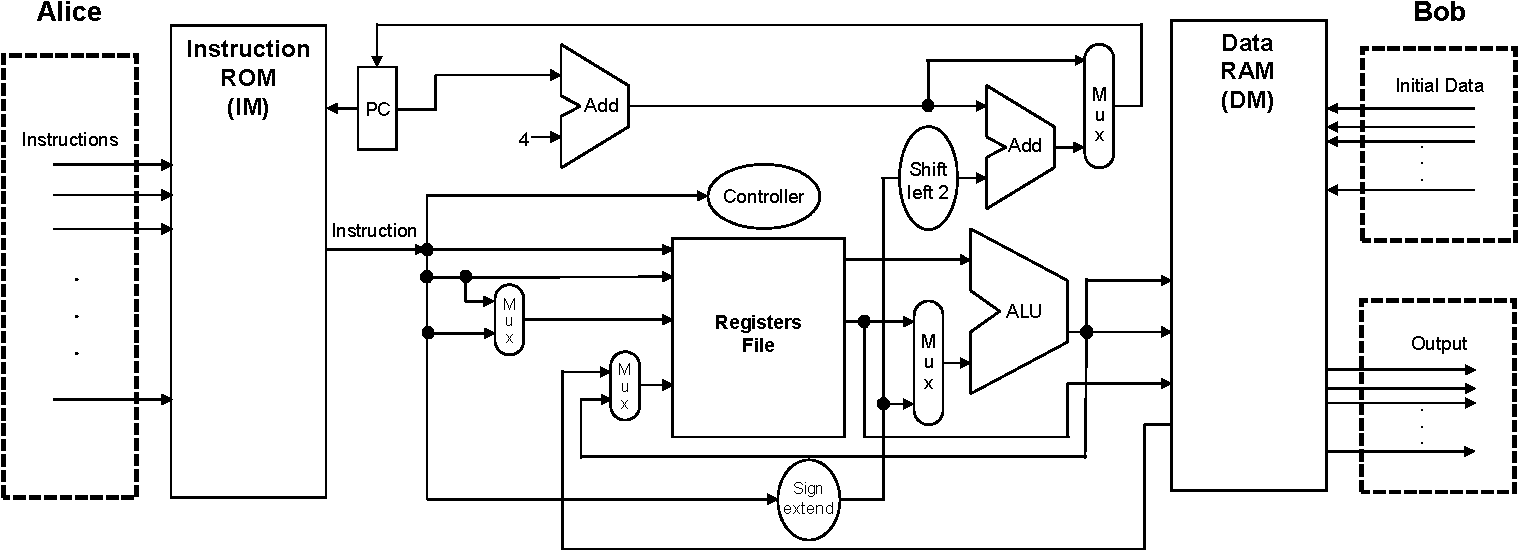
\includegraphics[width=0.95\textwidth]{mips-complex-crop.pdf}
\caption{Lite \gls{mips} architecture.
  Alice's and Bob's inputs and the output are shown.}\label{figure:mips}
\end{figure}

\fig{figure:mips} shows the overall architecture of our 32-bit \gls{mips} processor.
It is based on the Plasma project in opencores \cite{rhoads2006plasma}.
We modified the circuit such that the \acrshort{im} and the \acrshort{dm} are separated.
The original Plasma processor supports all the \gls{mips}~I \acrshort{isa} except unaligned memory access.
In our implementation, we also omit division instructions because of their large overhead.
Any arbitrary function described in \gls{c} language can be easily compiled to \gls{mips}~I assembly code using a cross-platform compiler, e.g., GNU gcc.

In 32-bit \gls{mips}, the \acrfull{pc} is a 32-bit register (array of \acrshort{ff}s) that points to the instruction that the processor is executing at the current cycle.
The processor fetches the instruction from the \acrshort{im} based on the current \acrshort{pc} value.
The \emph{controller} unit is responsible for setting signals to perform the instruction.
In 32-bit \gls{mips}, the \emph{register file} consists of 32 registers of 32-bit each.
In each cycle, at most two registers can be read and at most one register can be written back.
The \acrshort{alu} receives the read register(s) or a sign extended \textit{immediate} as operands.
The \acrshort{alu} also receives an opcode from the controller unit.
The output of the \acrshort{alu} will be either written back to the register file or fed to the \acrshort{dm} as an address for load/store.
The loaded data from the \acrshort{dm} is written back to the register file.
In each cycle, the processor increments the \acrshort{pc} by 4 to point to the next instruction in the \acrshort{im} or changes it according to a branch or jump instruction.

\section{Garbled Processor for SFE}\label{sec:processor-mips-sfe}
In the previous section, we discuss the idea of garbling a processor as a solution for hiding the function in \acrshort{pf-sfe}.
Besides enabling \acrshort{pf-sfe}, another advantage of a garbled processor is usability for non-expert users since it can be programmed using high-level languages, whereas other frameworks for the \acrshort{gc} protocol require tedious Boolean circuit construction.
However, garbling and evaluating the entire processor incurs a tremendous cost compared to \acrshort{sfe} solutions due to stronger privacy requirements in \acrshort{pf-sfe}.

In this section, we expand the garbled processor introduced in \sect{sec:processor-pro-pfsfe} and introduce a framework for secure computation that provides scalable support for generalized \acrshort{sfe}.
The framework provides three options: a high performance with a relaxed privacy setting, the more security-demanding \acrshort{pf-sfe} with a higher cost (similar to the one in \sect{sec:processor-pro-pfsfe}), and a flavor in-between.

To avoid information leakage about the function (i.e., \acrshort{pf-sfe}), we employ the \gls{mips} circuit with its full \acrfull{isa}, which incurs a substantial overhead due to garbling and evaluating of the entire \acrshort{isa}.
We can also compile the function using only a subset of the \acrshort{isa}: restricted \acrshort{isa} (i.e., semi-private function).
A third alternative is public function mode in which the function is compiled using only an application-specific subset of the \acrshort{isa} required for executing the function.
In the following, we discuss these modes of function evaluation and the trade-off between privacy and performance further.

\subsection{Garbled Processor for Public Functions}\label{ssec:processor-mips-sfe-public}
Employ a general-purpose processor supporting its entire \acrshort{isa} for \acrshort{sfe} incurs a significant computation and communication cost.
However, this cost seems unnecessary since both parties know the executed function instructions and they are only interested in learning the output value.
Hence, garbling a limited application-specific \acrshort{isa} for executing each instruction is sufficient to achieve the desired privacy.
To further reduce the \acrshort{isa}, assuming, for example, a function that consists of \numprint{10} instructions, we could theoretically generate $2^{10} -1$ \gls{netlist}s (\gls{netlist}s of \acrshort{isa} with different combinations of the 10 instructions, excluding the \gls{netlist} with zero instructions).
At run-time, one of these \gls{netlist}s is plugged in (garbled and evaluated) at each instruction step depending on the expected instructions.
However, to make it more reasonable (generate fewer \gls{netlist}s), for functions with control flow independent of private data, we know in advance which instruction will be executed at each step.
Thus, we need only the \gls{netlist} of the processor implementing \acrshort{isa} with that specific instruction, restricting the required \gls{netlist}s in this case to \numprint{10}.
For functions with control flow dependent on private data, a simple static analysis can be used to specify the combination of possible instructions at each step, and hence the required \acrshort{isa} \gls{netlist} as proposed in \cite{wang2016secure}.

\subsection{Garbled Processor for Semi-Private Functions}\label{ssec:processor-mips-sfe-semiprivate}
The main cost for garbling a processor with its entire \acrshort{isa} results from garbling circuits for expensive instructions like multiplication and division.
Most compilers can avoid these costly instructions and replace them with cheaper loops of shifts, addition, and subtraction instructions.
These replacements would eliminate the need for the Mult/Div unit in the processor and reduce the cost of garbling per instruction on the one hand.
However, on the other hand, one expensive instruction will be replaced with multiple cheap instructions, thus increasing the total number of instructions.
For example, multiplying two 32-bit numbers with the MULT instruction in \gls{mips} requires \numprint{15} cycles and a circuit of \numprint{13257} non-XOR gates\footnote{XOR gates are evaluated free of cost in \acrshort{gc} according to Free XOR \cite{kolesnikov2008improved}.}, while it requires at least \numprint{31} cycles and a circuit of \numprint{9,676} non-XOR gates when using a conditional loop over an ADD instruction.
We call this mode ``semi-private'' since it only reveals partial information about instructions executed in the program (that the program does not use division/multiplication) and increases the probability of guessing an instruction by reducing the subset of possible instructions (restricted \acrshort{isa}).

\subsection{Garbled Processor for Private Functions} \label{ssec:processor-mips-sfe-private}
In the standard 2-party \acrshort{pf-sfe}, Alice provides the function $g_{Alice}(\cdot)$, Bob provides the input data $b_{Bob}$, and the output is $g_{Alice}(b_{Bob})$.
Similar to \sect{sec:processor-pro-pfsfe}, the garbled processor receives a list of \emph{instructions} of compiled $g_{Alice}(\cdot)$ and applies them to the input data $b_{Bob}$ in memory, and eventually writes the output back to the memory.
To avoid information leakage about the private function, we use a general-purpose processor with its entire \acrshort{isa} (full \acrshort{isa}).

\subsection{Hardware Implementation of Garbled Processor} \label{ssec:processor-hardware}
To the best of our knowledge, the fastest implementation of \acrshort{gc} in hardware was~\cite{jarvinen2010garbled}.
However, their performance is far less than a JustGarble~\cite{bellare2013efficient}, a software implementation.
The reason for this gap is that JustGarble utilizes a more efficient fixed-key \acrshort{aes} for garbling instead of an expensive hash function.
Thus, it is possible that a hardware implementation leveraging the latest \acrshort{gc} optimizations including fixed-key \acrshort{aes} garbling would outperform the software implementation.
Furthermore, a processor is essentially a sequential circuit, and its evaluation requires sequential \acrshort{gc} which no hardware implementation of \acrshort{gc} supports.

We implement our \acrshort{gc} evaluator based on the most recent optimizations listed in \sect{ssec:prelim-imp}.
Its architecture is shown in \fig{fig:evaluator} and consists of:
(1) \acrfull{sscd} memory: a read-only memory that stores the information about gates in the \gls{mips} circuit in \acrshort{sscd} format (see \appx{sec:engine-sscd}).
(2) \acrshort{gc} Label memory: a read-write random-access memory that stores \acrshort{gc} labels of all wires in the corresponding \gls{mips} circuit.
(3) \acrfull{gt} memory: a read-write random-access memory that stores the garbled tables of each non-XOR gate in the \gls{mips} circuit that are generated by Alice (garbler).
(4) Sequential Handler: a controller that supports evaluation of the sequential circuits with the \acrshort{gc} protocol.
(5) Evaluator Core: the implementation of the core functionality of Yao’s \acrshort{gc} protocol's evaluation, its most recent optimizations \cite{kolesnikov2008improved, bellare2013efficient, zahur2015two}, and the sequential garbling presented in \chap{chap:seq}.

As shown in \fig{fig:evaluator}, Bob's input labels in the Label memory are initialized by the \acrshort{ot} protocol with Alice.
The rest of the labels in the Label memory and the Garbled Tables memory are received from Alice.

\begin{figure}
\centering
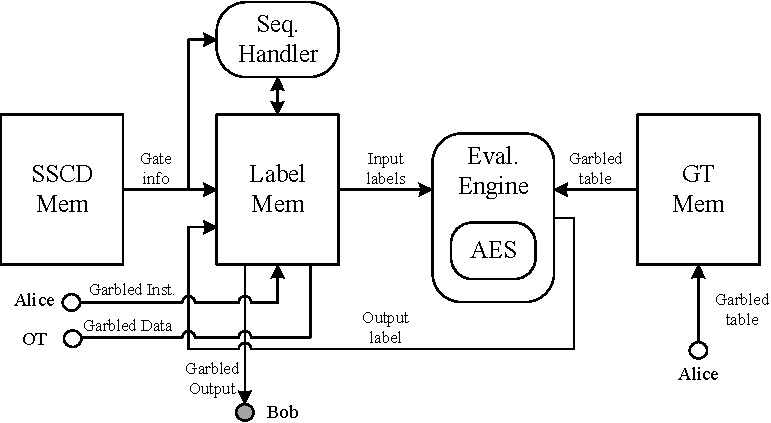
\includegraphics[width=0.8\textwidth]{evaluator-crop.pdf}
\caption{Architecture of our hardware \acrshort{gc} Evaluator.}
\label{fig:evaluator}
\end{figure}

\subsubsection{Pipelined Evaluator Core and Gate Dependency} \label{ssec:processor-hardware-pipeline}
To maximize the performance of our hardware \acrshort{gc} evaluator, we use a 20-stage pipelined \acrshort{aes} implementation \cite{hsing2013tiny} inside our Evaluator Core module.
It increases the throughput of the module by increasing the maximum operating clock frequency of the core.
We also add one stage for the rest of the \acrshort{gc} evaluation functionality.

Due to Free XOR \cite{kolesnikov2008improved}, evaluating an XOR gate requires only XORing the input labels while evaluating a non-XOR gate requires two \acrshort{aes} encryptions \cite{zahur2015two}.
Therefore, the Evaluator Core can finish the evaluation of an XOR gate in one clock cycle of the pipeline.
The different timing for XOR and non-XOR gates introduces a challenge for handling dependencies of gates' inputs and output.
A gate cannot enter the evaluation pipeline if its inputs are another gate's output which is not yet evaluated.
Stalling pipeline is a naive approach for resolving this dependency and degrades the overall performance
To mitigate this, we push XOR gates to the latest empty stage of the pipeline such that the subsequent dependent gates can enter the pipeline as soon as possible.

\subsubsection{Extending Hardware Prototype} \label{ssec:processor-hardware-extend}
In this thesis, we only use on-chip memory for as a proof-of-concept implementation.
However, this prototype can be extended to support interfacing with off-chip memory which would store garbled tables and labels of larger garbled processor circuits and functions.
It can also interface with another \acrshort{fpga} emulator of the garbler which generates the garbled tables and labels and streams them to our evaluator.
A wide range of scenarios is now feasible owing to our current hardware platform and state-of-the-art optimized \acrshort{gc} evaluator.

Such extensions would incur additional area and performance overheads but would allow upscaling of our implementation to support garbled processor circuits and benchmarks in the Gigabytes range.
We emphasize that we provide in this thesis a proof-of-concept prototype to motivate further research in this direction to bring garbled processors some steps closer to the realm of efficient and practical implementations.

\section{ARM2GC: Garbled ARM for SFE}\label{sec:processor-arm}
In this section, we present \gls{arm2gc}, a \acrshort{gc} framework based on a garbled \gls{arm} processor and the \gls{skipgate} algorithm.
The framework aims to simplify the development of privacy-preserving applications while keeping the garbling cost as low as the best optimized garbled circuits.
We first describe the overview of \gls{arm2gc} and its \acrshort{api} for \acrshort{gc} development.
Then, we explain how \gls{arm}'s unique architecture helps to decrease garbling overhead.
Next, the effect of \gls{skipgate} in reducing the garbling cost is discussed.
Finally, we discuss why we do not employ \acrshort{oram} for \gls{arm2gc}.

\subsection{Global Flow}\label{ssec:arm-global}
The \gls{arm2gc} framework allows users to write two-party \acrshort{sfe} program in \gls{c}/C++ (or any language that can be compiled to \gls{arm} binary code).
\fig{fig:frwk_overview} shows the overview of the framework.
The framework benefits from the \gls{skipgate} algorithm to reduce the cost of garbling the \gls{arm} processor.
As described in \chap{chap:skipgate}, the \gls{skipgate} algorithm supports secure evaluation of circuits in the form of $f(a,b,p)$ where $a$ and $b$ are Alice's and Bob's inputs, and $p$ is a public input known to both parties.
In the \gls{arm2gc} framework, the circuit $f(\cdot,\cdot,\cdot)$ is the circuit of \gls{arm} processor and the public input $p$ is the compiled binary code of the user's \acrshort{sfe} program.
To avoid confusion with \gls{arm} circuit, we denote the user's function with $g$.
Similar to other two-party \acrshort{sfe} functions, $g(\cdot,\cdot)$ has two inputs, one from Alice and one from Bob.
The high-level code of $g(\cdot,\cdot)$ is compiled using an \gls{arm} cross-compiler, e.g., gcc-arm-linux-gnueabi.
The compiled binary code of $g(\cdot,\cdot)$ is then passed to the \gls{arm} circuit as the public input $p$.
The parties' private inputs ($a$ and $b$) are passed directly to \gls{arm} circuit: $f(a,b,p)$.
The \gls{skipgate} algorithm then securely evaluate $f(a,b,p)$ by reducing the circuit into the simpler circuit of $f_{p}(a,b) = f(a,b,p)$.
The \gls{arm} circuit computes the function $g(\cdot,\cdot)$ on the private inputs and returns its output: $o = f(a,b,p) = g(a,b)$.

\begin{figure}
\centering
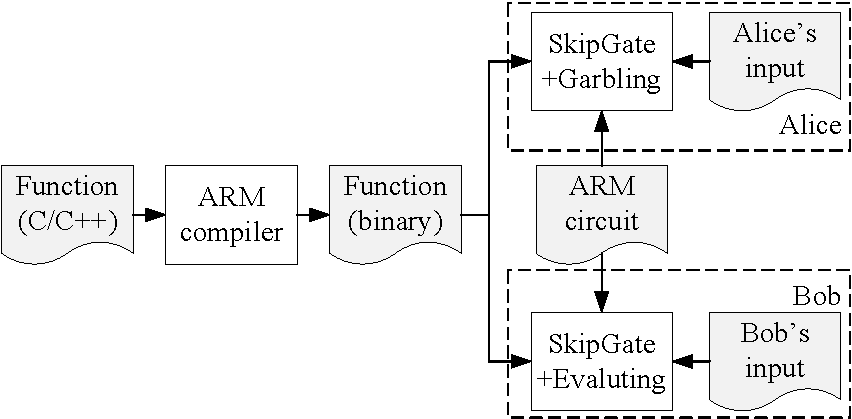
\includegraphics[width=0.7\textwidth]{frwk_overview-crop.pdf}
\caption{Overview of the \gls{arm2gc} framework.}\label{fig:frwk_overview}
\end{figure}

The \gls{arm2gc} framework supports the following \acrshort{api} in \gls{c} language for the user's function $o = g(a,b)$:
\begin{lstlisting}[language=C,basicstyle=\ttfamily,keywordstyle=\color{blue}\ttfamily,stringstyle=\color{red}\ttfamily,commentstyle=\color{CommentColor}\ttfamily]
void gc_main(
  const int *a,// Alice's input
  const int *b,// Bob's input
  int *c) {// output array
  // The user's code goes here.
}
\end{lstlisting}

The entry function, \texttt{gc\_main}, receives three arguments: pointers to Alice's input, Bob's input, and the output.
The circuit of our \gls{arm} processor has five separate memory elements (consisting of \acrshort{ff}s and \acrshort{mux}s) to store: Alice's inputs, Bob's inputs, output, stack, and instructions.
The \acrshort{ff}s in the instruction memory are initialized with the compiled binary code that is known to both parties (the public input $p$).
The flip-flops in Alice's and Bob's memories are initialized with labels corresponding to their private inputs $a$ and $b$ respectively.
The other \acrshort{ff}s in the stack, output, pipeline registers, and the register file are initialized to zero.
The \gls{arm} circuit is garbled using sequential garbling process of \gls{tinygarble} \acrshort{gc} engine (see \appx{chap:engine}) for a pre-specified number of sequential cycles $cc$.

A signal called \textit{terminate} is produced by the \gls{arm} circuit that indicates if \texttt{gc\_main} function is returned.
The signal can be revealed to the parties once in $K$ cycles (predetermined by parties) to reduce the total number of cycles of garbling the \gls{arm} circuit.
For $K=1$, the parties instantly identify the termination, but the exact number of cycles the function evaluated for the given inputs is revealed.
A larger $K$ would reduce this information leakage, but increase the garbling cost.
\appx{chap:engine} provides more details about the support of the terminate signal in \gls{tinygarble} \acrshort{gc} engine.
Eventually, when the function is executed, the parties reveal the content of the output memory to each other to learn output $o = g(a,b)$.

\subsection{ARM as a Garbled Processor}\label{ssec:arm}
In this thesis, we choose \gls{arm} as the garbled processor which is a more ubiquitous and sophisticated processor compared to \gls{mips}.
\gls{arm} has two primary advantages:
(1) Pervasiveness: the compilers and toolsets of \gls{arm} are under constant scrutiny, updating, and probably, more optimized as a result.
(2) Conditional Execution: Designed to improve the performance and code density, conditional execution allows \gls{arm} to execute each instruction only if a specific condition is satisfied~\cite{sloss2004arm}.

\gls{arm} compilers tend to replace conditional branches with conditional instructions to make the flow of the program predictable, and thus, lower the cost of branch mis-prediction.
Similarly, in the garbled processor, the main design effort is to make sure that the flow of the program is predictable so that the next instruction remains public.
Replacing conditional branches with conditional instructions in garbled \gls{arm} generates a code with a predictable flow.
\fig{fig:conditional_exec} shows an example function compiled into assembly with and without the conditional execution.
Moreover, we modify the \gls{arm} controller such that conditional instructions always take the same number of cycles regardless of their condition (taken or not taken).
Otherwise, the program flow will be dependent on the secret condition, and as a result, the program flow itself will become secret which in turn reduces the efficiency of the execution.

\begin{figure}
    \centering
    \begin{subfigure}{0.40\columnwidth}
        \centering
        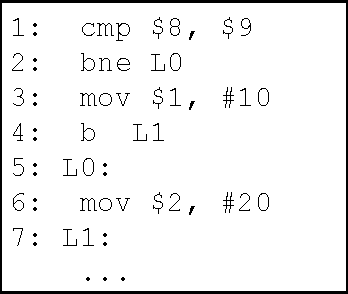
\includegraphics[width=\textwidth]{conditional_exec_wo-crop.pdf}
        \caption{Without Conditional Execution}
    \end{subfigure}
    ~
    \begin{subfigure}{0.40\columnwidth}
        \centering
        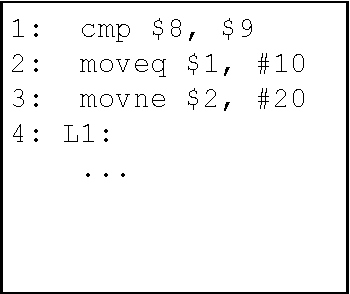
\includegraphics[width=\textwidth]{conditional_exec_w-crop.pdf}
        \caption{With Conditional Execution}
    \end{subfigure}
    \caption{An example code showing how conditional execution in \gls{arm} can reduce the code size and make the program flow predictable.}\label{fig:conditional_exec}
\end{figure}

We modify and remove a few features from the \gls{arm} processor like interrupts, co-processors, and performance-related components including cache and pipeline.
The last group does not bring any performance advantages in the \acrshort{gc} protocol, as the circuit is garbled/evaluated gate by gate (serially).
Note that unlike in hardware, the performance of \acrshort{gc} does not increase by parallelizing gates in the circuit.
In the \acrshort{gc} protocol, the total number of non-XOR gates is the only factor affecting the performance, not the circuit's topology.

Implementation of the \gls{arm} processor results in a complex and large circuit (containing almost five times more gates than the \gls{mips} processor).
Thus, using \gls{arm} instead of \gls{mips} would incur even a higher cost.
However, the majority of the components of the \gls{arm} processor remain idle during  execution of an instruction.
In the next section, we describe how \gls{skipgate} utilizes this characteristic to minimize the cost of garbling the \gls{arm} processor.

\subsection{How {SkipGate} Helps}
As explained above, we initialize the instruction memory of the \gls{arm} with public values.
Therefore, if the program counter (the address of the next instruction) is public, the next instruction becomes public as well.
As a result, the control path also becomes public, and \gls{skipgate} can easily detect the idle components to mark them for skipping.
Moreover, due to \gls{skipgate}, the gates of the active components that are only transporting data between memory, register file, and \acrshort{alu} act as wires and do not incur any cost.
According to \gls{skipgate}'s notation, the \gls{arm} Boolean circuit is a 3-input function $o = f(a,b,p)$ where $p$ is equal to the compiled binary code of $g(a,b)$ and $a$ and $b$ are the parties' private inputs.
\gls{skipgate} reduces the \gls{arm} circuit into a smaller circuit of $o = f_p(a,b)$ where $f_p$ can perform the exact operation required in the function $g(\cdot,\cdot)$.
Therefore, the main garbling cost is paid only for the actual computation of the secret values.
As explained in the previous section, \gls{skipgate} performs these optimizations at the gate-level, in contrast to instruction-level of the approaches in \sect{sec:processor-mips-sfe} and \cite{wang2016secure}.

\subsection{Why not Sub-linear ORAM?}
As mentioned in \sect{ssec:arm-global}, we use an array of \acrshort{mux}s and \acrshort{ff}s to implement the register file in \gls{arm} circuit.
This structure means that the cost of accessing the register file, when performed obliviously, is linear with respect to its size.
One natural question would be why we did not employ \acrfull{oram} that enables oblivious access to memories in the \acrshort{gc} protocol with sub-linear cost~\cite{wang2014scoram, zahur2016revisit}.
The reason is that, in most cases, the access to the register file is not required to be oblivious.
Since the instructions come from the publicly known instruction memory, both parties know which register of the register file is read or written.
The \gls{skipgate} algorithm utilizes this to skip garbling of the gates in the \acrshort{mux}s of the register file.
Thus, no cost is required for such accesses.
With \acrshort{oram}, all the accesses to the register file would be the costly oblivious access of \acrshort{oram}.

In rare occasions where two or more instructions should be garbled at a time, accessing a register would not be free using \acrshort{mux}s and \gls{skipgate}.
These cases only happen when \gls{arm} compiler fails to replace a conditional branch on a secret value with conditional instructions.
The user can typically alter the program in a way that the compiler avoids such branches and replaces it with conditional instructions instead.
However, in these cases, the \gls{skipgate} algorithm removes most of the gates in the register file.
Since the cost of fetching instructions remains smaller than that of break-even points of sub-linear \acrshort{oram}s, using \acrshort{oram} would not improve the efficiency for this case either.

\begin{figure}
\centering
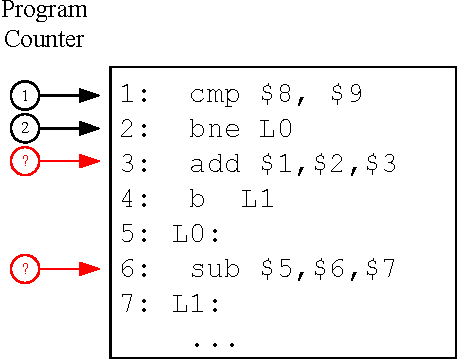
\includegraphics[width=0.5\textwidth]{branch-crop.pdf}
\caption{In case of compiler failure to replace a secret branch with conditional instructions, the parties do not know which instruction is executed after the branch.
Thus, the instruction becomes secret.}
\label{fig:branch}
\end{figure}

\fig{fig:branch} shows an example where after execution of a branch on a secret value, the next instruction becomes secret and unknown to parties.
In this example, the program counter can be either 3 or 6 depending on the outcome of the comparison in Line 1.
Thus, two instructions \texttt{add \$1, \$2, \$3} (\texttt{\$3 = \$1 + \$2}) and \texttt{sub \$5, \$6, \$7} (\texttt{\$5 = \$6 - \$7}) have to be garbled/evaluated at the same time.
For fetching the second register in instruction from the register file, we only have two choices: \texttt{\$2} and \texttt{\$6}.
This limited choice means that, instead of having a complete oblivious access to the register file with 16 options, we only have to select obliviously between 2 of the 16 registers.
This cost is far less than 1-out-of-16 oblivious access.
The cost of oblivious access using \acrshort{mux}s and \gls{skipgate} to a \textit{subset} of memory is equal to an oblivious access to a memory with the size of the subset.

\begin{figure}
\centering
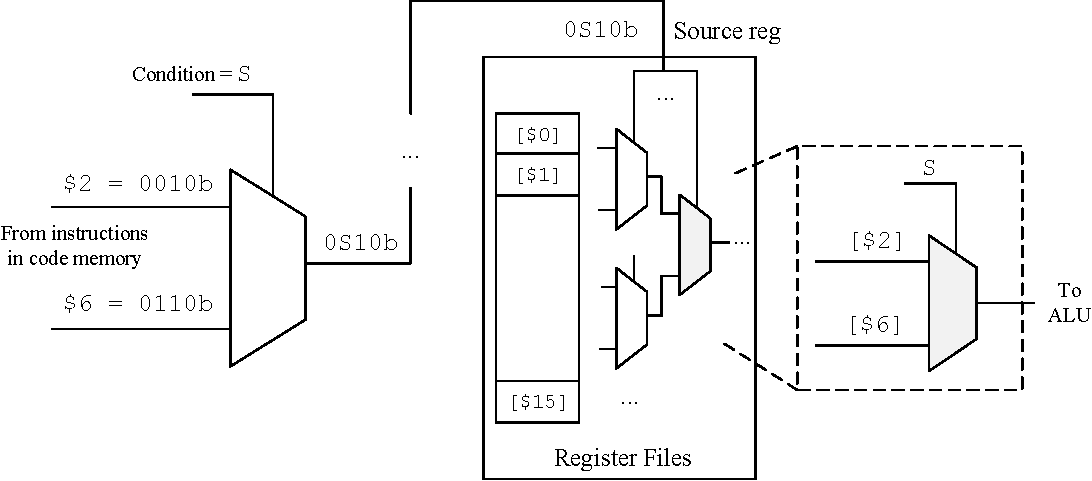
\includegraphics[width=0.9\textwidth]{registers-crop.pdf}
\caption{Bit-precise details of how source register is fetched while executing two instructions \texttt{add \$1, \$2, \$3} and \texttt{sub \$5, \$6, \$7} at the same time after a branch on a secret condition value \texttt{S}.}
\label{fig:registers}
\end{figure}

\fig{fig:registers} illustrates the details of the above example where bit \texttt{S} is the secret bit that separates the branches of computation that each is leading into a different instruction.
The address of the source register is computed by a \acrshort{mux} over the two options in the two instructions: \acrshort{mux}(\texttt{\$2, \$6, S}) = \acrshort{mux}(\texttt{0010b, 0110b, S}) = \texttt{0S10b}.
The most and least significant bits are, in either case, zero, and thus it will remain zero in the output.
The bit 1 is one in both cases and remains one.
The bit 2 is zero if \texttt{S==0} and is one if \texttt{S==1}, and thus this bit is equal to \texttt{S}.
Now, let us look at the \acrshort{mux}s in the registers files that fetch the source register.
The \acrshort{mux}s connected to the known bit can be evaluated separately by both parties, and thus \gls{skipgate} will avoid garbling/evaluating them.
Within the \acrshort{mux}s connected to \texttt{S}, only the one that selects between \texttt{[\$2]} and \texttt{[\$6]} remains for garbling, and \gls{skipgate} will skip the rest due to non-positive fanout.

% why not \acrshort{oram} for code and data memory
The rationale for using an array of \acrshort{mux}s in the register file also applies to the code, data, and stack memories where the access is almost always public and known to both parties.
In the worst case, only a subset of memory is accessed obliviously, thus making the cost of memory access below the threshold of switching to \acrshort{oram}s.

% Research question
The mixture of the \gls{skipgate} algorithm and garbled processor introduces an unusual use-case for oblivious memory where oblivious access is performed only on a varying subset of the memory.
The subset can be different from one access to the other.
The current sub-linear \acrshort{oram} protocols cannot address this scenario efficiently.
Thus, an interesting research question is raised:

\textbf{Is it possible to \textit{obliviously} access (read/write) a varying subset of the memory with a \textit{sub-linear} cost in terms of the subset size?}

% !TEX root = 0_main.tex
\chapter{Evaluation}
We use a variety of benchmark functions to evaluate the performance and practicability of TinyGarble.
In this section, we first describe our experimental setup (\sect{sect:exp}) and metrics for quantifying the performance of TinyGarble (\sect{ssect:metrics}).
We outline the performance comparison of TinyGarble (with HDL synthesizer and our custom libraries) on combinational benchmark functions with PCF \cite{kreuter2013pcf}, one of the best known earlier automated methodologies to generate circuits for garbling in \sect{ssect:customlib}.
TinyGarble's performance in generating sequential circuits for benchmark functions using a standard HDL synthesis tool is demonstrated in \sect{ssect:seqeval}.
\sect{ssect:cacheTime} shows the CPU time for various numbers of sequential cycles which demonstrates the effect of memory footprint reduction in garbling time.
\sect{ssect:HLSeval} shows a comparison between TinyGarble's performance using an HLS tool (input written in C) and using a conventional HDL synthesis tool (input given in Verilog).
Lastly, \sect{ssect:mipsres} shows the result of our garbled processor and implementation of Hamming distance as a benchmark.

We also compare the performance of the commercial logic synthesis tool with the academic, open-source tools in Appendix \ref{app:seqos}.
We show that in most cases, the performance of the open-source tool is comparable to the commercial tool.

\section{Experimental Setup}
The circuit generations are all done on a system with Linux RedHat Server 5.6, 8~GB of memory, and Intel Xeon X5450 CPU @ 3~GHz.
We use another system with Ubuntu 14.10 Desktop, 12.0~GB of memory, and Intel Core i7-2600 CPU @ 3.4GHz to assess the timing performance of the sequential garbling scheme in \sect{ssect:cacheTime}.

Two sets of HDL synthesis tool chains are used in our experiments: one commercial and one open-source (Appendix \ref{app:seqos}).
Our commercial HDL level synthesis tool is Synopsis Design Compiler (DC) 2010.03-SP4 \cite{tool:DesignCompiler}.
We also use the Synopsis Library Compiler from the DC package to interpret our custom technology library.
In \sect{ssect:HLSeval}, we utilize Xilinx Vivado HLS \cite{tool:Vivado}, a commercially available HLS tool whose inputs are written in the C/C++ programming language.
We emphasize that TinyGarble can operate with any commercial or open-source sequential HDL-level (or HLS) synthesizer, as long as the synthesizer is capable of performing state-of-the-art logic optimization and mapping algorithms.

\section{Performance Metrics}
We use the following metrics to measure the efficiency of TinyGarble for generating garbled circuits:

\begin{itemize}
\item
	\textit{Memory Footprint Efficiency} ($\mathit{MFE}$): $$\mathit{MFE} = \dfrac{q_{0}}{q},$$ where $q_{0}$ is the total number of gates in the reference circuit and $q$ is the total number of gates in the circuit under evaluation.
	The maximum number of tokens that need to be stored at any point during garbling/evaluation as well as memory required for storing circuit description is directly proportional to the number of gates in both sequential and combinational circuits.
	Thus, the total number of gates is approximately proportional to the memory footprint.

\item
	\textit{Number of Garbled Tables} ($\mathit{\#GT}$): $$\mathit{\#GT} = \#nonXOR\times c,$$ where $\#nonXOR$ is the number of non-XOR gates in a circuit and $c$ is the number of sequential cycles that the circuit needs to be garbled/evaluated.
	In free XOR-based GC schemes, each non-XOR gate requires a garbled table to be generated by the garbler and sent to the evaluator at each sequential cycle.
	Thus, this metric is an estimate of both the computation and communication time.

\item
	\textit{Garbled Tables Difference} ($\mathit{GTD}$ (\%)): $$\mathit{GTD} = \dfrac{\mathit{\#GT} - \mathit{\#GT}_{0}}{\mathit{\#GT}_{0}} \times 100,$$ where $\mathit{\#GT}_{0}$ is the total number of garbled tables for the reference circuit and $\mathit{\#GT}$ is the total number of garbled tables for the circuit under evaluation.
	When comparing a sequential with a combination circuit, positive $\mathit{GTD}$ shows an \emph{overhead} (caused by folding a circuit with an asymmetric loop, see \sect{sect:sequen}) in total computation and communication time resulting from an excessive number of garbled tables generated in the sequential circuits.
	However, in general, negative $\mathit{GTD}$ shows improvement in the number of non-XOR gates and generated garbled tables that results from logic synthesis optimization.
\end{itemize}

\section{Benchmark functions}
We evaluate TinyGarble's circuit generation method on various benchmark functions.
Several of these functions have been used in previous works, e.g., PCF~\cite{kreuter2013pcf}.
In the following, we introduce our benchmarks and explain how we fold them into a sequential representation.

\textit{Sum.} This function receives two $N$-bit inputs and outputs an $N$-bit sum.
The sum function is implemented in $N$ steps of one bit sums by keeping the carry bit.
Thus, it can be folded up to $N$ times without any significant overhead in number of garbled tables ($\mathit{\#GT}$).

\textit{Hamming Distance.} This function receives two $N$-bit inputs and outputs the $\log_2(N)$-bit Hamming distance between them.
The Hamming distance between two numbers is the number of positions at which the corresponding bits are different.
A possible combinational implementation of the $N$-bit Hamming distance uses a binary tree of adders that sums all $1$-bit values from the bit differences to a final Hamming distance consisting of $\log_2(N)$ bits \cite{boyar2006concrete}.
This implementation cannot be folded easily.
However, we can fold this function into $N$-cycles of one XOR and one $\log_2(N)$-bit adder.
This causes an overhead compared to the combinational circuit.

\textit{Compare (Millionaires problem).} This function receives two $N$-bit unsigned input values and outputs a greater than signal consisting of one bit that indicates if the first input is greater than the second one.
The comparison function can be implemented in $N$ steps of subtraction by keeping the carry bit \cite{kolesnikov2009improved}.
Thus, it can be folded up to $N$ times without any significant overhead.

\textit{Multiplication.} This function receives two unsigned $N$-bit inputs and outputs their unsigned $N$-bit product.
The multiplication function consists of $N$ additions and shifts.
The shift operations result in an asymmetric structure in this function.
Thus, folding it up to $N$ times may increase the overhead.

\textit{Matrix Multiplication.} This function receives two $N\times N$ matrices consisting of $32$-bit unsigned numbers and outputs an $N\times N$ matrix equal to the product of the input matrices.
The $N\times N$ matrix multiplication function consists of three $N$-cycle nested loops with a symmetric structures.
It can be folded up to $N^3$ times without any significant overhead.

\textit{AES-128.} This function receives a 128-bit plaintext and 128-bit round keys and outputs a 128-bit ciphertext based on the Rijndael algorithm.
The AES-128 function consists of 10 rounds with almost symmetric structure.
Ideally, it can be folded up to $10$ times without any significant overhead.

\textit{SHA3.} This function receives $576$-bit inputs and outputs a $1600$-bit number equal to the SHA3 hash of the input.
We implement the Keccak-f permutations[$1600$] procedure for realizing this function.
The SHA3 function consists of 24 steps, each with a symmetric structure.
It can be folded 24 times without any significant overhead.

\section{Combinational Garbled Circuit}
To show the performance gain of using our custom libraries, we compare TinyGarble combinational circuits with circuits reported in PCF \cite{kreuter2013pcf}.
We choose PCF because among the \emph{automated} GC tools available at the time of writing, it shows better results for most of the benchmarks.
In some other work like FastGC \cite{huang2011faster}, a number of benchmark circuits have been more aggressively improved (compared to PCF) using ad-hoc and mostly manual optimizations, but without a generalizable methodology.

The comparison is shown in \tab{table:result-comb}.
We compute the garbled tables difference $\mathit{GTD}$ (see \sect{ssect:metrics}) of various benchmarks by using circuits reported in PCF as reference ($\mathit{GTD}$\textsuperscript{PCF}).
It can be seen that the combinational circuits generated by TinyGarble have non-positive $\mathit{GTD}$\textsuperscript{PCF} which means that the number of garbled tables are less than or equal to that of PCF circuits.
We also compare the memory footprint by computing the memory footprint efficiency $\mathit{MFE}$ with PCF as reference ($\mathit{MFE}$\textsuperscript{PCF}).
We observe that $\mathit{MFE}$\textsuperscript{PCF} is larger than 1 (up to 9.3).
This means that even without using sequential circuits, the memory footprint can be reduced by almost an order of magnitude by using TinyGarble custom libraries and standard HDL synthesis.

In case of Hamming distance, TinyGarble shows, on average, $80\%$ improvement in number of garbled tables.
Another automated tool CBMC-GC \cite{franz2014cbmc} reports better result compared to PCF for Hamming 160 (non-XOR $\numprint{4738}$, total gates $\numprint{20356}$).
However, TinyGarble shows $66\%$ improvement in number of garbled tables compared to CBMC-GC.
In case of 256-bit and 1024-bit Multiplication, and $8\times 8$ and $16\times 16$ Matrix Multiplication, because of the huge (impractical) sizes, Synopsis DC was unable to generate the entire combinational circuit.
This is because Synopsis DC is a tool developed for commercial applications.
The real-life applications are almost always written sequentially, otherwise the design would not be scalable or even amenable to offline compilation onto a hardware circuit.
We emphasize that our sequential circuit ($c>1$) provides the exact same functionality while having a very small memory footprint compared with the reference circuit.

\subsection{Comparison with Hand-Optimized Circuits}
The netlists generated by the automated flow of TinyGarble show similar performance as the hand-optimized netlists in many cases.
For example, \cite{kolesnikov2009improved} describe an $N$-bit sum circuit with $5N$ gates of which $N$ gates are non-XOR and an $N$-bit comparison circuit with $4N$ gates of which $N$ gates are non-XOR.
The circuits generated by TinyGarble have about the same number of gates for these two functions.
Note that one can always add any hand-optimized module to the synthesis library of TinyGarble.

\section{Sequential Garbled Circuit}
As described in \sect{sect:sequen}, the user has the degree of freedom to fold a combinational circuit and convert it to a sequential one to reduce the memory footprint.
$c$ denotes the number of sequential cycles required to garble/evaluate the circuit.
This value demonstrates the amount of folding that is performed before the circuit is input to the synthesizer.
The user defines the value of $c$ and writes her own input function in an HDL or a higher level language such that the function is evaluated in $c$ sequential cycles.

We use Memory Footprint Efficiency ($\mathit{MFE}$), to evaluate the reduction in memory requirement.
We use TinyGarble combinational circuits ($c=1$) as reference.
The ideal $\mathit{MFE}$ for a circuit with $c$ sequential cycles is $c$.
We also compare the memory footprints of sequential circuits with combinational circuits reported in PCF ($\mathit{MFE}$\textsuperscript{PCF}).

As explained in \sect{ssect:sqcirc}, the folding process may introduce some overhead on the total number of garbled tables.
To assess this overhead, we compute the Garbled Tables Difference ($\mathit{GTD}$) of the sequential circuit using TinyGarble combinational circuits as reference.
The ideal $\mathit{GTD}$ is $0\%$, which means that the total number of garbled tables should be equal to those for a functionally equivalent combinational circuit.
We also compare the number of garbled tables of sequential circuits with combinational circuits reported in PCF ($\mathit{GTD}$\textsuperscript{PCF}) to show that even with the incurred overhead, the number of garbled tables for sequential circuits is still less than that of PCF for most cases.

\begin{table*}
\centering
\caption{Comparison of TinyGarble combinational circuits with PCF.
In case of AES 128, the result is compared with FastGC.}
\label{table:result-comb}
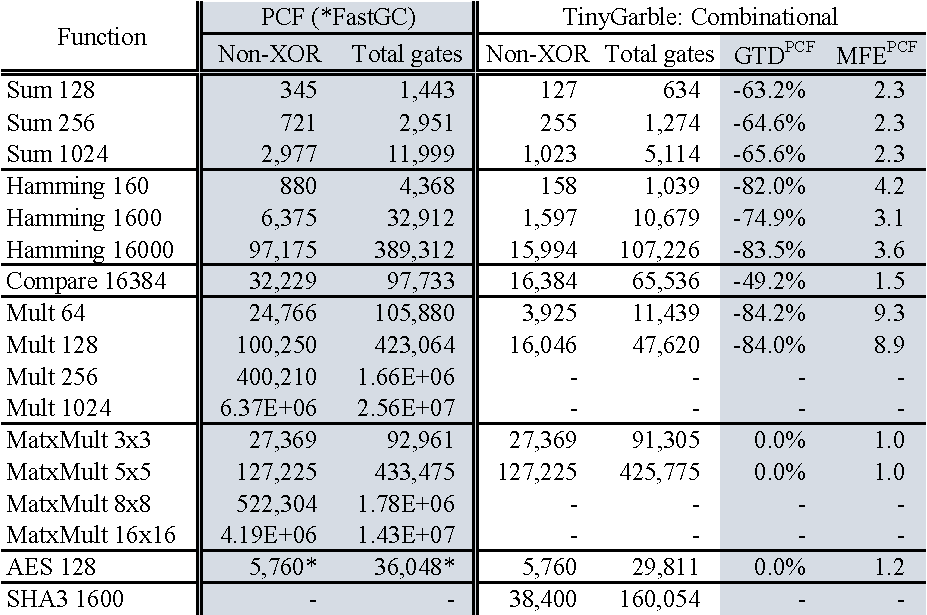
\includegraphics[width=0.7\textwidth]{results-comb-crop.pdf}
\end{table*}

\begin{table*}
\centering
\caption{Comparison of TinyGarble sequential circuits with PCF and TinyGarble combinational circuits.
In case of AES 128, the result is compared with FastGC.}
\label{table:result-seq}
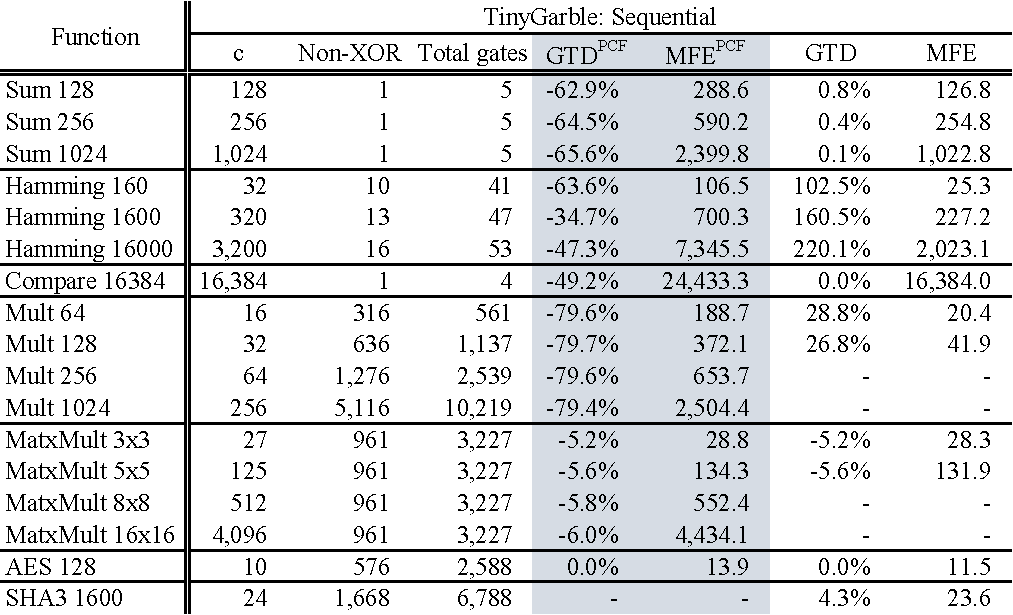
\includegraphics[width=0.7\textwidth]{results-seq-crop.pdf}
\end{table*}

\tab{table:result-seq} shows the number of total gates, non-XOR gates, $\mathit{MFE}$, $\mathit{GTD}$, $\mathit{MFE}$\textsuperscript{PCF}, and $\mathit{GTD}$\textsuperscript{PCF} of the benchmark circuits for various input widths.
$\mathit{MFE}$, $\mathit{GTD}$ are computed with TinyGarble combinational circuits (with $c=1$) as reference.
$\mathit{MFE}$\textsuperscript{PCF}, and $\mathit{GTD}$\textsuperscript{PCF} use the circuits reported in PCF as reference.
In the case of AES 128, we compare our implementation with the manually optimized circuit reported in FastGC \cite{huang2011faster} because PCF did not report it directly.

We provide a few highlights from \tab{table:result-seq}.
TinyGarble is able to decrease the size of the sum of two $1024$-bit numbers by $\numprint{1022.8}$ times (i.e., more than three orders of magnitude) without affecting the number of garbled tables ($\mathit{GTD}$) compared with its own combinational circuit.
For Hamming 16000, TinyGarble is able to decrease the memory footprint by $\numprint{7345.5}$ times (i.e., about 4 orders of magnitude) while reducing the number of garbled tables by $47.3\%$ in comparison with the circuit reported in PCF.
In case of Mult 1024, TinyGarble shrinks the memory footprint by a factor of $\numprint{2504.4}$ while reducing the number of garbled tables by $79.4\%$ when compared with the result in PCF.
For a $16\times 16$ matrix multiplication, a $\numprint{4434.1}$ more compact TinyGarble solution with $6\%$ less garbled tables compared with PCF is available.
By folding AES-128 10 times, the total number of gates is reduce by a factor of $13.9$ compared to the  FastGC circuit without any overhead in the number of non-XORs.
Observe that the savings are typically more for larger bit-widths while extreme foldings can introduce an increased overhead in number of garbled tables due to the resulting asymmetry.

Because of the TinyGarble superior scalability, we are able to implement functions that have never been reported before, such as SHA-3, which can be represented using $\numprint{344059}$ and $\numprint{6788}$ gates respectively.

\section{Effect of Folding on Garbling Time}
So far, we have only reported the overhead in terms of garbled tables ($\mathit{GTD}$) that is a function of the number of non-XOR gates.
As explained in \cite{bellare2013efficient}, if we see garbling as a cryptographic primitive, its computation time (without considering communication) will also be interesting.
In practice, smaller circuits which can fit entirely in the processor cache result in fewer cache misses and therefore, consume less CPU cycles for garbling.
To better observe the impact of cache speed-up for the compact circuits resulting from TinyGarble, \fig{fig:cpu_time} depicts the CPU Time (left y-axis) and the memory footprint of wire tokens (right y-axis) versus $c$ (x-axis) for the $\numprint{32768}$-bit Sum function.
As mentioned earlier, the memory footprint is directly proportional to the total number of gates in the sequential circuit.

This experiment is done using our sequential garbling scheme based on JustGarble \cite{bellare2013efficient} that includes using Free XOR, Row Reduction, and Fixed-key AES garbling techniques (see \sect{subsect:preli_GC}).
We use an Intel Core i7 CPU @ 3.40GHz which supports the AES-NI instruction set.
The CPU cycle is measured as the average of $10,000$ trials using RDTSC instruction.
For security parameter $k=128$ (the bit-width of wire token, see \sect{subsect:preli_GC}), we store $128$-bit per tokens.
For garbling in JustGarble, we store 2 tokens, 2 32-bit input indexes, and an 8-bit gate-type per gate.
Thus, the memory footprint is approximately $328$-bit per gate in garbling operation.
Folding the circuit by a factor of $c \in [1:\numprint{32768}]$ constantly decreases the memory footprint while the computation effort remains almost constant.
Interestingly, as can be seen from the figure, the number of CPU cycles sharply decreases by $1.6\times$ just when we fold four times ($c=4$) compared to $c=1$.
This is because for $c \geq 4$, the memory space required for garbling completely fits in the cache.
The minimum CPU cycle per gate happens at $c=\numprint{2048}$ for $3.2$~KB memory footprint.
This signifies the fact that even for large functions, we can use the sequential approach to fit the corresponding memory space requirement into the cache and avoid the penalty of cache misses, thus achieving a large reduction in garbling time.

\begin{figure}[ht]
	\centering
	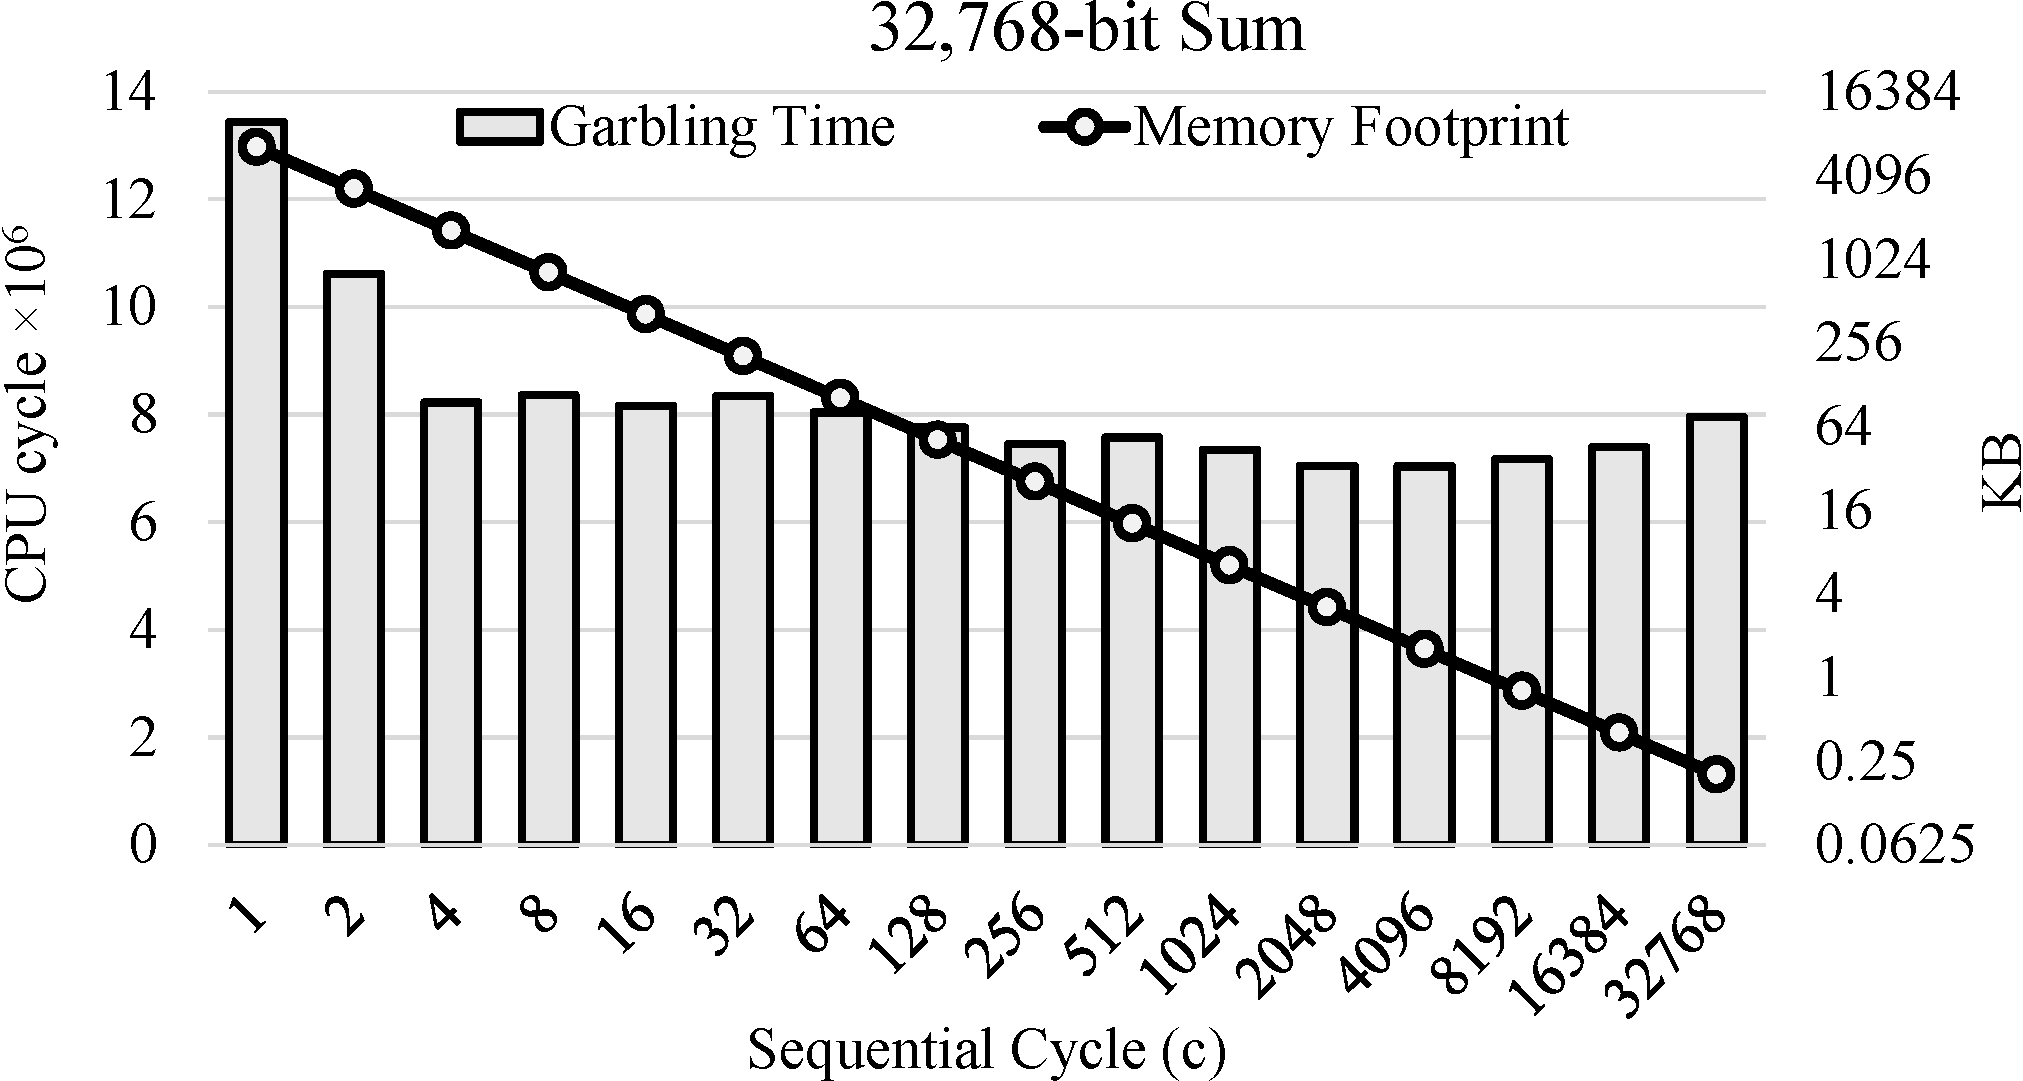
\includegraphics[width=0.7\textwidth]{CPU_Time-crop.pdf}
	\caption{Garbling $\numprint{32768}$-bit Sum function.
The CPU time in number of cycles and the approximate memory footprint in KBytes (y-axis) versus $c$ (x-axis) are shown.}
	\label{fig:cpu_time}
\end{figure}

\section{High Level Synthesis Tools}
The design automation community has been working on tools that work with higher-level languages and abstractions than HDL.
While a host of commercial and academic HLS tools are available \cite{tool:Vivado, tool:PandA, decaluwe2004myhdl, Gupta2004}, we selected the Xilinx Vivado HLS for compiling C code to HDL which can then be synthesized using a conventional HDL synthesis tool.
The HLS engine in the Vivado suite is built upon the xPilot project \cite{Chapter:Zhang2008}.

\begin{table*}[t]
\centering
\caption{Comparison of performance of the circuits generated using C input to HLS and a direct Verilog input to the HDL synthesizer.}
\label{table:hls}
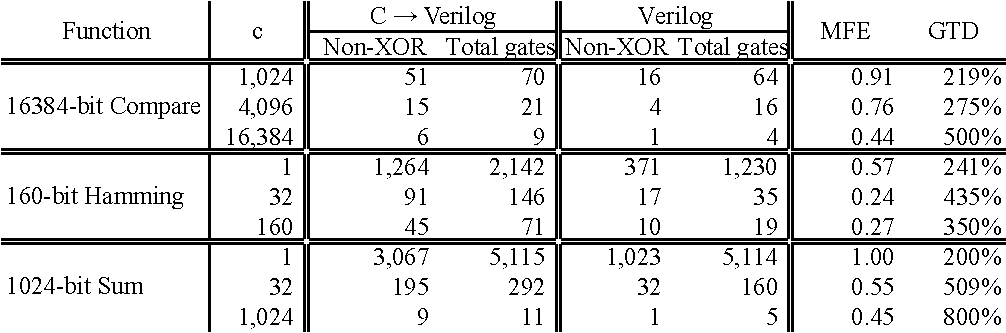
\includegraphics[width=0.7\textwidth]{HLS-crop.pdf}
\end{table*}

Table \ref{table:hls} demonstrates a comparison between the performance of the circuits generated using C input to the HLS tool (C$\rightarrow$Verilog) and a direct Verilog input.
As can be seen from the table, the resulting memory footprint could increase by a factor between 1 and 4, while the number of garbled tables varies in a range of 3 to 9 times.
It is well known that writing the HDL level code which contains the time information and more detailed structural/behavioral description would yield much more efficient circuits than the code written in a higher level language.

\section{Evaluation of MIPS}
We implement general purpose processor for PF-SFE using MIPS~I where one user provide function description in assembly and the other provides the data.
Support of sequential circuits in TinyGarble enables us to use the MIPS circuit description in Plasma project \cite{rhoads2006plasma} without major modifications.
In the following, we provide the result of MIPS implementation and its memory footprint and communication load.
Lastly, we present implementation of Hamming distance with variable input length as a benchmark of private function application on MIPS.

\subsection{MIPS Implementation}
We used TinyGarble to generate the netlist for the MIPS sequential circuit.
\tab{table:mipsres} shows the total number of gates and non-XOR gates for each module of the MIPS processor with $64\times32$bit DM and IM.
The sum of non-XORs for each module is $\numprint{14997}$.
However, when the modules are combined together to form the entire MIPS processor, the synthesizer optimizes the circuit such that the total number of non-XORs is reduced by $14.95\%$ to $\numprint{12755}$.
The memory footprint for storing tokens during garbling MIPS is approximately the size of two tokens times the total number of gates which is $2 \times 128 \times \numprint{31719}$bit $=991$~KB for token bit-width $k=128$.
The communication load between parties for invocation of one instruction (one sequential cycle) is approximately the size of three tokens times the number of non-XOR gates which is $3\times 128 \times \numprint{12755}$bit $=598$~KB with Row Reduction optimization.

\begin{table}[ht]
\centering
\caption{Number of total gates and non-XOR gates in the MIPS implementation.
The global optimization of TinyGarble reduces the overall number of gates compared to that of the sum of individual modules.}\label{table:mipsres}
\begin{tabular}{l|rrl}
Modules             & Total gates & Non-XOR \\ \hline \hline
Controller          & 509                                                  & 470                                                \\
Bus                 & 603                                                  & 590                                                \\
ALU                 & 651                                                  & 346                                                \\
Shifter             & \numprint{1362}                                                 & \numprint{1092}                                               \\
Mult                & \numprint{2147}                                                 & \numprint{1792}                                               \\
Reg File            & \numprint{8880}                                                 & \numprint{3023}                                               \\
IM                  & \numprint{6048}                                                 & \numprint{2016}                                               \\
DM                  & \numprint{13779}                                                & \numprint{5423}                                               \\
PC                  & 309                                                  & 245                                                \\ \hline
Total               & \numprint{34288}                                                & \numprint{14997}                                              \\ \hline \hline
MIPS                & \numprint{31719}                                                & \numprint{12755}                                              \\ \hline \hline
\begin{tabular}[c]{@{}l@{}}Global \\optimization\end{tabular} & 7.49\%                                               & 14.95\%
\end{tabular}
\end{table}

\subsection{Benchmark: Hamming Distance}
We implemented the Hamming distance function as a proof-of-concept for our secure MIPS.
It counts the number of different elements in two arrays $A$ and $B$ with variable length $l$.
For the hand-optimized assembly code shown in \fig{figure:hamminassembly}, the function requires at most $7+9l$ sequential cycles (instructions) to evaluate.
Thus, based on \tab{table:mipsres}, this function requires overall $\numprint{12755}\times(7+9l)$ non-XOR gates.
It has only $16$ instructions and is stored in $16\times32$bit of the IM.
The function requires that $l$, $A$, and $B$ are stored in addresses $0$, $[2:l+1]$, and $[l+2:2l+1]$ of DM respectively.
It will store the Hamming distance of $A$ and $B$ in address $1$.

\begin{figure}[ht]
\lstinputlisting{Hamming.s}
\caption{Hamming distance assembly code.}\label{figure:hamminassembly}
\end{figure}

\section{Open Source Logic Synthesis Tools}
TinyGarble offers a generic methodology for generating GC that is transparent to the underlying logic synthesis tool.
To show this point, we demonstrate an implementation of TinyGarble using the Yosys \cite{tool:Yosys} and ABC \cite{tool:ABC} logic synthesis tool chain for circuit generation.
Both of these tools are open-source and available online.
We compare the performance of the commercial HDL synthesis tool, i.e., Synopsys DC, with this open-source synthesis tool chain.
ABC is an academic package developed at the University of California Berkeley.
Yosys is an HDL-based synthesis tool which calls ABC for its technology mapping.
The HDL inputs for describing both sequential and combinational circuits are written in the Verilog programming language.

We compare the performance of these open-source tools to the commercially available Synopsys DC.
The results are presented in \tab{table:abc}.
For comparison purposes, we compute $\mathit{GTD}$ and $\mathit{MFE}$ using the netlists generated by Synopsys DC as reference.
For most of the benchmarks $\mathit{GTD}$s are either very small or zero which implies that the number of non-XOR gates in circuits generated by Yosys and by Synopsys DC are almost similar.
In terms of memory footprint, different tools perform better for different benchmark functions.
These results shows that TinyGarble is transparent to the underlying logic synthesis tool as long as the tool is up to date with respect to the known methods for logic minimization and mapping.
Since the logic synthesis tools perform a series of optimizations, they may use different (heuristic) algorithms for some of their internal steps which could lead to slightly different results.
A user can choose between different synthesis tools based on their performance and availability.

\begin{table}[ht]
\caption{Comparison of circuit generation performance between the commercial Synopsys DC and Yosys+ABC open source logic synthesizer.}
\label{table:abc}
\centering
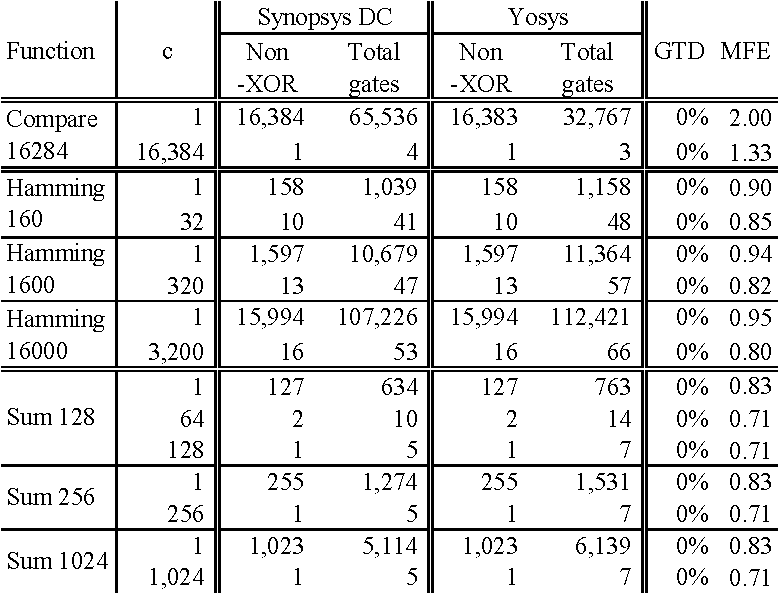
\includegraphics[width=0.7\textwidth]{abc-crop.pdf}
\end{table}

\section{Evaluation Setup of GarbledCPU}\label{ssect:evalset}
We create different instances of a single-cycle MIPS architecture with specific, restricted, and full IS to support a trade-off between efficiency and privacy. (Full IS was proposed in \cite{songhori2015tinygarble} and is reported for comparison.) The different MIPS instances are synthesized using Synopsys Design Compiler DC H-2013.03-SP4 to generate optimized sequential Boolean circuits. These circuits are then evaluated on our hardware GC evaluator implemented using Vivado 2014.4.1 on a Xilinx Virtex-7 FPGA.

\section{Benchmarks}\label{ssect:bench}
As benchmarks we used Hamming distance, private set intersection and AES. We compile these benchmarks from high-level C to MIPS binary using a MIPS cross-compiler. For some benchmarks, assembly code manipulation allows to reduce the number of clock cycles required. To assure correctness of both benchmarks and IS under test, we simulate the resulting binary file using the Modelsim simulator and calculate the number of required cycles to compute each of the benchmarks, reported in~\tab{tab:cyc_bench}, for accurate performance measurements. For Hamming distance, the number of cycles depends on the size of the input strings. In the PSI benchmark, we compute a variant of PSI called PSI cardinality (PSI-CA) where only the number of common elements is revealed. The sets can have different sizes where each element is 32-bit.  For AES, we assume that one party holds a 128-bit message and the other party holds eleven round keys each of 128-bit length to avoid unnecessary garbling and evaluation of the round-key generation function.

\begin{table}[ht]
\caption{Number of required cycles to compute benchmarks.}\label{tab:cyc_bench}
\centering
\small
\begin{tabular}{l|r|r}
\multicolumn{1}{c|}{Benchmark} & \multicolumn{1}{c|}{Input Size} &  \multicolumn{1}{c}{\# of required cycles} \\
\hline
\hline
Hamming Distance & $\numprint{16}$ & $\numprint{218}$\\
\hline
 Hamming Distance & $\numprint{32}$ & $\numprint{426}$\\
\hline
Hamming Distance & $\numprint{64}$ & $\numprint{842}$\\
\hline
Hamming Distance & $\numprint{128}$ & $\numprint{1674}$\\
\hline
PSI & $\numprint{64}$ &$\numprint{7267}$\\
\hline
PSI & $\numprint{128}$ &$\numprint{14267}$\\
\hline
AES (no key expansion) & $\numprint{128}$ & $\numprint{6178}$\\
\end{tabular}
\end{table}

\section{Synthesis of the GarbledCPU IS}
We synthesize the MIPS architecture, shown in~\fig{figure:mips}, with Synopsys DC for different ISs and memory sizes: 32 to 512 32-bit words for instruction and data memories. Generating these Boolean circuits is a one-time process and the circuits can be re-used without incurring further compilation costs. \tab{tab:synres} shows the synthesis time and number of non-XOR gates of the IS's with different sizes of memories.

\begin{table}[ht]
\caption{Synthesis results of different variants of (IS)}\label{tab:synres}
\centering
\begin{tabular}{l|r|r|r}
\multicolumn{1}{c|}{Memory Size} & \multicolumn{1}{c|}{Synthesis Time} &  \multicolumn{1}{c|}{\# of Combinatorial} & \multicolumn{1}{c}{\# of Sequential} \\
\multicolumn{1}{c|}{(words)} & \multicolumn{1}{c|}{seconds (s)} &  \multicolumn{1}{c|}{non-XOR gates} & \multicolumn{1}{c}{gates} \\
\hline
\hline
\multicolumn{4} {c}{Hamming Distance-specific IS}\\
\hline
DM, IM = 32 & $\numprint{19.648}$~$s$ & $\numprint{6715}$ & $\numprint{2021}$ \\
\hline
DM, IM = 64 & $\numprint{31.692}$~$s$ & $\numprint{9830}$ & $\numprint{3046}$ \\
\hline
DM, IM = 128 & $\numprint{62.212}$~$s$ & $\numprint{16062}$ & $\numprint{5095}$ \\
\hline
DM, IM = 256 & $\numprint{167.398}$~$s$ & $\numprint{28493}$ & $\numprint{9192}$ \\
\hline
DM, IM = 512 & $\numprint{589.186}$~$s$ & $\numprint{53374}$ & $\numprint{17385}$ \\
\hline
\multicolumn{4} {c}{PSI-specific IS}\\
\hline
DM, IM = 32 & $\numprint{18.735}$~$s$ & $\numprint{6751}$ & $\numprint{2021}$ \\
\hline
DM, IM = 64 & $\numprint{31.117}$~$s$ & $\numprint{9866}$ & $\numprint{3046}$ \\
\hline
DM, IM = 128 & $\numprint{61.551}$~$s$ & $\numprint{16097}$ & $\numprint{5095}$ \\
\hline
DM, IM = 256 & $\numprint{163.564}$~$s$ &$\numprint{28529}$ & $\numprint{9192}$ \\
\hline
DM, IM = 512 & $\numprint{591.145}$~$s$ & $\numprint{53410}$ & $\numprint{17385}$ \\
\hline
\multicolumn{4} {c}{AES-specific IS}\\
\hline
DM, IM = 256 & $\numprint{169.498}$~$s$ &$\numprint{32177}$ & $\numprint{9214}$ \\
\hline
DM, IM = 512 & $\numprint{594.047}$~$s$ & $\numprint{61570}$ & $\numprint{17406}$\\
\hline
\multicolumn{4} {c}{ALU\&Shift IS}\\
\hline
DM, IM = 32 & $\numprint{21.681}$~$s$ & $\numprint{9676}$ & $\numprint{2046}$ \\
\hline
DM, IM = 64 & $\numprint{34.588}$~$s$ & $\numprint{12702}$ & $\numprint{3070}$ \\
\hline
DM, IM = 128 & $\numprint{65.873}$~$s$ & $\numprint{19694}$ & $\numprint{5118}$ \\
\hline
DM, IM = 256 & $\numprint{170.974}$~$s$ &$\numprint{34071}$ & $\numprint{9214}$ \\
\hline
DM, IM = 512 & $\numprint{593.945}$~$s$ & $\numprint{66238}$ & $\numprint{17406}$ \\
\hline
\multicolumn{4} {c}{ALU-only IS}\\
\hline
DM, IM = 32 & $\numprint{19.599}$~$s$ & $\numprint{8136}$ & $\numprint{2046}$ \\
\hline
DM, IM = 64 & $\numprint{31.970}$~$s$ & $\numprint{11696}$ & $\numprint{3070}$ \\
\hline
DM, IM = 128 & $\numprint{62.599}$~$s$ & $\numprint{18816}$ & $\numprint{5118}$ \\
\hline
DM, IM = 256 & $\numprint{164.894}$~$s$ &$\numprint{33041}$ & $\numprint{9214}$ \\
\hline
DM, IM = 512 & $\numprint{598.986}$~$s$ & $\numprint{65183}$ & $\numprint{17406}$ \\
\hline
\multicolumn{4} {c}{Full IS~\cite{songhori2015tinygarble}}\\
\hline
DM, IM = 32 & $\numprint{38.331}$~$s$ & $\numprint{13257}$ & $\numprint{2110}$ \\
\hline
DM, IM = 64 & $\numprint{50.446}$~$s$ & $\numprint{16818}$ & $\numprint{3134}$ \\
\hline
DM, IM = 128 & $\numprint{82.863}$~$s$ & $\numprint{23899}$ & $\numprint{5182}$ \\
\hline
DM, IM = 256 & $\numprint{189.157}$~$s$ &$\numprint{38118}$ & $\numprint{9278}$ \\
\hline
DM, IM = 512 & $\numprint{616.750}$~$s$ & $\numprint{69423}$ & $\numprint{17470}$ \\
\end{tabular}
\end{table}


\begin{itemize}
\item \emph{Application-specific IS for public functions:} We synthesized three variants of the application-specific IS where the selected instructions include only the ones used by a particular function, for various memory sizes. We create the application-specific IS for the three benchmarks: Hamming distance\footnote{\small{Instructions required for \emph{Hamming distance} are:} \tiny{LW, SW, ADD, SUB, XOR, NOP, SLL and BEQ}}, PSI\footnote{\small{Instructions required for \emph{PSI} are:} \tiny{LW, SW, ADD, SUB, NOP, SLL, BEQ, BNE and SLT}}, and AES\footnote{ \small{Instructions required for \emph{AES} are:} \tiny{LW, LB, SW, SB, ADD, SUB, AND, XOR, OR, NOP, SLL, SRL, BEQ, BNE, JAL, JR and SLT}}.
\item \emph{Restricted IS for semi-private functions:} We synthesized two variants of the restricted IS: one without the Mult/Div unit and another without Mult/Div and Shift units. Since the difference between the two depends mainly on reducing the control logic and select lines of multiplexers, the numbers of non-XOR gates for both are different. However, the number of flip-flops are the same.
\item \emph{Full IS~\cite{songhori2015tinygarble} for private functions:} We show full IS synthesis results with different memory sizes in \tab{tab:synres}.
\end{itemize}

\section{Performance Evaluation}
\subsection{Area} \tab{table:resource} shows the resource allocation and utilization of our GC Evaluator on a Xilinx Virtex-7 FPGA. Note that the FPGA utilization does not vary for different memory sizes and instances of the MIPS processor since the evaluator logic remains unaltered. For different memory sizes and IS instances, only the non-XOR gate count varies. This only impacts the garbled labels and tables memory which significantly affects the off-chip memory utilized for storing the garbled tables, and the Block Random-Access Memory (BRAM) resources utilization only to a small extent.

\begin{table}[ht]
\centering
\caption{Resource allocation and utilization of GarbledCPU GC Evaluator on a Xilinx Virtex-7 FPGA.}
\label{table:resource}
\begin{tabular}{l|r|r}
Resource    & \multicolumn{1}{c|}{Estimation} & \multicolumn{1}{c}{Utilization \%} \\ \hline \hline
Flip-Flop (FF) & $\numprint{22035}$ & $\numprint{2.54}$ \\ \hline
Slice LookUp Table (LUT) & $\numprint{21229}$ & $\numprint{4.90}$ \\ \hline
BRAM & $\numprint{354}$ & $\numprint{24}$
\\ \hline
BUFG & $\numprint{2}$ & $\numprint{6.25}$
 \end{tabular}
\end{table}

\subsection{Performance} \tab{table:performance} presents the runtime required to evaluate GarbledCPU for one instruction in terms of clock cycles and $\mu\textrm{s}$. Our GC evaluator operates at $100\textrm{MHz}$ on the FPGA. This is used to compute an average evaluation runtime of 1.1 clock cycles per gate for our pipelined GC evaluator which translates to an average of $11\textrm{ns}$ per gate in our FPGA implementation. The reported runtime can be further improved by providing tighter timing constraints.

\subsection{Comparison with Other Work}
\tab{tab:comp} shows a comparison with other GC evaluator implementations. However, for fairness, we are leveraging GC optimizations that were not available at the time for \cite{jarvinen2010garbled}. We compare with our two implementations, the 21-stage pipelined evaluator and un-pipelined variant to show the effect of pipelining in improving our performance by a factor of 7.8. \tab{tab:comp} compares our results with interpolated results estimated for other works. Results indicate that our pipelined GC evaluator FPGA implementation takes $51\times$ fewer clock cycles compared to the fastest software implementation JustGarble \cite{bellare2013efficient}. Although the CPU clock frequency ($3.0\textrm{GHz}$) is $30\times$ faster than that of our Virtex-7 FPGA ($100\textrm{MHz}$), our pipelined implementation would still be almost $2\times$ faster than JustGarble in terms of absolute time. Note that our implementation is just a prototype on a reconfigurable FPGA as opposed to a custom design of Intel AES-NI in CPU. Implementing GarbledCPU on an ASIC would improve its performance in terms of absolute time even further. Moreover, our implementation is two orders of magnitude faster than the previously fastest hardware implementation of \cite{jarvinen2010garbled}.

\begin{table}[ht]
\centering
\caption{Performance of GarbledCPU for different (ISs) with different memory sizes at $100\textrm{MHz}$ clock frequency.}\label{table:performance}
\begin{tabular}{l|r|r|r|r|r}
\multicolumn{1}{c|}{Memory Size (words)} & \multicolumn{1}{c|}{$\numprint{32}$ } &  \multicolumn{1}{c|}{$\numprint{64}$ } & \multicolumn{1}{c|}{$\numprint{128}$ } & \multicolumn{1}{c|}{$\numprint{256}$ } & \multicolumn{1}{c}{$\numprint{512}$ }  \\ \hline \hline
\multicolumn{6} {c}{Hamming Distance-IS}\\ \hline
\# of non-XOR gates       & $\numprint{6715}$    & $\numprint{9830}$   & $\numprint{16062}$ & $\numprint{28493}$ & $\numprint{53374}$\\ \hline
Time per inst. (cc)       & $\numprint{7118}$    & $\numprint{10813}$ & $\numprint{17829}$ & $\numprint{30773}$  & $\numprint{57644}$\\ \hline
Time per inst. ($\mu s$) & $\numprint{71.18}$  & $\numprint{108.13}$  & $\numprint{178.29}$  & $\numprint{307.72}$  & $\numprint{576.44}$\\ \hline
Avg. Time per gate (cc)  & $\numprint{1.06}$      & $\numprint{1.10}$   & $\numprint{1.11}$    & $\numprint{1.08}$  & $\numprint{1.08}$\\ \hline
\multicolumn{6} {c}{PSI-IS}\\ \hline
\# of non-XOR gates       & $\numprint{6751}$    & $\numprint{9866}$   & $\numprint{16097}$ & $\numprint{28529}$ & $\numprint{53410}$\\ \hline
Time per inst. (cc)       & $\numprint{7426}$    & $\numprint{10952}$ & $\numprint{18029}$ & $\numprint{30811}$  & $\numprint{57149}$\\ \hline
Time per inst. ($\mu s$) & $\numprint{74.26}$  & $\numprint{109.52}$  & $\numprint{180.29}$  & $\numprint{308.11}$  & $\numprint{571.49}$\\ \hline
Avg. Time per gate (cc)  & $\numprint{1.10}$      & $\numprint{1.11}$   & $\numprint{1.12}$    & $\numprint{1.08}$  & $\numprint{1.07}$\\ \hline
\multicolumn{6} {c}{AES-specific IS}\\ \hline
\# of non-XOR gates       & - & -&- & $\numprint{32177}$   & $\numprint{61570}$\\ \hline
Time per inst. (cc)       &-  & -&- & $\numprint{35717}$   & $\numprint{68343}$\\ \hline
Time per inst. ($\mu s$) & - & -& -& $\numprint{357.17}$ & $\numprint{683.43}$ \\ \hline
Avg. Time per gate (cc)  & -&- &- & $\numprint{1.11}$      & $\numprint{1.11}$ \\ \hline
\multicolumn{6} {c}{ALU\&Shift-IS}\\
\hline
\# of non-XOR gates       & $\numprint{9676}$    & $\numprint{12702}$ & $\numprint{19694}$ & $\numprint{34071}$  & $\numprint{66238}$\\ \hline
Time per inst. (cc)       & $\numprint{10644}$  & $\numprint{13972}$ & $\numprint{22057}$ & $\numprint{36115}$  & $\numprint{71537}$\\ \hline
Time per inst. ($\mu s$) & $\numprint{106.44}$ & $\numprint{139.72}$  & $\numprint{220.57}$  & $\numprint{361.15}$  & $\numprint{715.37}$\\ \hline
Avg. Time per gate (cc)  & $\numprint{1.10}$     & $\numprint{1.10}$   & $\numprint{1.12}$    & $\numprint{1.06}$  & $\numprint{1.08}$\\ \hline
\multicolumn{6} {c}{ALU-only IS}\\
\hline
\# of non-XOR gates       & $\numprint{8136}$    & $\numprint{11696}$   & $\numprint{18816}$  & $\numprint{33041}$ & $\numprint{65183}$\\ \hline
Time per inst. (cc)       & $\numprint{8624}$  & $\numprint{12866}$ & $\numprint{21074}$  & $\numprint{35684}$  & $\numprint{73657}$\\ \hline
Time per inst. ($\mu s$) & $\numprint{86.24}$ & $\numprint{128.66}$     & $\numprint{210.74}$  & $\numprint{356.84}$  & $\numprint{736.57}$\\ \hline
Avg. Time per gate (cc)  & $\numprint{1.06}$     & $\numprint{1.10}$    & $\numprint{1.12}$    & $\numprint{1.08}$  & $\numprint{1.13}$\\ \hline
\multicolumn{6} {c}{Full IS~\cite{songhori2015tinygarble}}\\
\hline
\# of non-XOR gates       & $\numprint{13257}$    & $\numprint{16818}$   & $\numprint{23899}$ & $\numprint{38118}$ & $\numprint{69423}$\\ \hline
Time per inst. (cc)       & $\numprint{14848}$  & $\numprint{18668}$ & $\numprint{25811}$ & $\numprint{40786}$  & $\numprint{77060}$\\ \hline
Time per inst. ($\mu s$) & $\numprint{148.48}$ & $\numprint{186.68}$  & $\numprint{258.11}$  & $\numprint{407.86}$  & $\numprint{770.60}$\\ \hline
Avg. Time per gate (cc)  & $\numprint{1.12}$     & $\numprint{1.11}$   & $\numprint{1.08}$    & $\numprint{1.07}$  & $\numprint{1.11}$\\
\end{tabular}
\end{table}

\begin{table}[ht]
\centering
\caption{Comparing our GC evaluator implementation with other works' estimation for MIPS with 64-word memory.}\label{tab:comp}
\begin{tabular}{l||r|r}
\multicolumn{1}{c||}{Method} & \multicolumn{1}{c|}{\begin{tabular}[c]{@{}c@{}}Total time\\(cc)\end{tabular}} & \multicolumn{1}{c}{cc/gate} \\ \hline \hline
J\"arvinen et al. (SoC)~\cite{jarvinen2010garbled} & $\numprint{37329233}$ & $\numprint{2219.6}$ \\ \hline
J\"arvinen et al. (Stand-Alone FPGA)~\cite{jarvinen2010garbled} & $\numprint{4291954}$ & $\numprint{255.2}$ \\ \hline
JustGarble (CPU)~\cite{bellare2013efficient} & $\numprint{948535}$ & $\numprint{56.4}$ \\ \hline
Our work w/o pipeline & $\numprint{144635}$ & $\numprint{8.6}$ \\ \hline
Our work w/ pipeline & $\numprint{18500}$ & $\numprint{1.1}$
\end{tabular}
\end{table}

\section{Evaluation of ARM2GC}\label{sec:eval}
We also compare the overall performance of our GarbledCPU with the performance of the proposed software solution in \cite{wang2015secure} on the compatible benchmarks. For computing Hamming distance on two 32-bit integer arrays, Wang et al.'s solution takes $1.24s$ to garble 481K gates (see Table 4 in \cite{wang2015secure}). GarbledCPU requires \numprint{6715} non-XOR gates and \numprint{426} cycles (see Tables \ref{tab:synres} and \ref{tab:cyc_bench}), and thus it takes only $0.0314s$ to evaluate 2.8M gates. Given that garbling time is double the evaluation time, this indicates a speedup of factor 18 for GarbledCPU but with $6\times$ more AND gates for the same functionality. In terms of throughput, GarbledCPU can evaluate 90.8M gates and Wang et al.'s solution can evaluate 776K gates which makes GarbledCPU 117 times faster owing to our hardware implementation. However, this speedup assumes on-chip memory and is likely to be much smaller when utilizing off-chip memory.

\subsection{Evaluation Setup}
We use Synopsis Design Compiler (DC) H-2013.03-SP4~\cite{tool:DesignCompiler} along with TinyGarble~\cite{songhori2015tinygarble} synthesis and technology libraries to generate the netlists for the benchmark circuits and the ARM processor.

For the ARM2GC framework, we use the Amber ARM project, an open-source implementation of ARM v2a ISA on opencores~\cite{santifort2010amber}.
The ARM circuit is modified as explained in \sect{ssec:arm}.
Synthesizing the ARM processor with Synopsis DC takes few hours.
However, the process is done only once for a given memory size and it can be used for any set of functions and inputs afterwards.
The benchmark functions for ARM2GC are implemented in C and compiled using GNU gcc-arm-linux-gnueabi (Ubuntu/Linaro 5.3.1-14ubuntu2).
We used \texttt{-Os} compiler optimization flag in order to reduce the number of instructions.
We modified the header assembly code to change the addresses of stack, code, and data memories in the compiled binary.
We do not apply any optimization on the binary code.
Thus, similar to a normal software compilation, it takes less than a few seconds to compile a function into an ARM binary code.

\subsection{Benchmark Functions and Metrics}
We use the benchmark functions that have been frequently used for evaluation in the GC literature~\cite{holzer2012secure, songhori2015tinygarble, wang2015secure}. The benchmarks are as follows:

\begin{itemize}
\vspace{-0.06in}
\item Sum adds two integers.
\vspace{-0.1in}
\item Compare compares two integers.
\vspace{-0.1in}
\item Hamming finds the Hamming distance between two integers.
\vspace{-0.1in}
\item Mult calculates the product of two integers.
\vspace{-0.1in}
\item MatrixMult$N\times N$ computes matrix multiplication of two $N\times N$ matrices.
\vspace{-0.1in}
\item SHA3 finds SHA3-256 hash of a string.
\vspace{-0.1in}
\item AES computes AES-128 encryption given two 128-bit numbers as the key and the message.
\end{itemize}

%Metric
The most important metric to compare the cost of garbling is the total number of garbled non-XOR gates.
This metric encompasses both the cost of computation (encrypting/decrypting garbled tables) and the cost of communication (transferring garbled tables) in the GC protocol \cite{kolesnikov2008improved}.

\begin{table}
\centering
\caption{SkipGate algorithm improvement on sequential circuits generated by TinyGarble (TG)~\cite{songhori2015tinygarble}. These functions do not have public inputs. SkipGate benefits from the small number of flip-flops initial values that are public to reduce their garbling cost.}\label{tab:sys_impvoment}
\resizebox{\columnwidth}{!}{%
\begin{tabular}{l||r|r|r||r}
\multirow{2}{*}{Function (bit)} & \multicolumn{2}{c|}{\# of garbled non-XOR} & \multicolumn{1}{c||}{\multirow{2}{*}{\begin{tabular}[c]{@{}c@{}}\# of skipped\\ non-XOR\end{tabular}}} & \multicolumn{1}{c}{\multirow{2}{*}{Improv.}} \\ \cline{2-3}
 & \multicolumn{1}{c|}{TG~\cite{songhori2015tinygarble}} & \multicolumn{1}{c|}{SkipGate} & \multicolumn{1}{c||}{} & \multicolumn{1}{c}{} \\ \hline \hline
Sum 32 & 32 & 31 & 1 & 3.1\% \\
Sum 1024 & 1,024 & 1,023 & 1 & 0.1\% \\
Compare 32 & 32 & 32 & 0 & 0.0\% \\
Compare 16,384 & 16,384 & 16,384 & 0 & 0.0\% \\
Hamming 32 & 160 & 145 & 15 & 9.4\% \\
Hamming 160 & 1,120 & 1,092 & 28 & 2.5\% \\
Hamming 512 & 4,608 & 4,563 & 45 & 1.0\% \\
Mult 32 & 2,048 & 2,016 & 32 & 1.6\% \\
MatrixMult3x3 32 & 25,947 & 25,668 & 279 & 1.1\% \\
MatrixMult5x5 32 & 120,125 & 119,350 & 775 & 0.6\% \\
MatrixMult8x8 32 & 492,032 & 490,048 & 1,984 & 0.4\% \\
SHA3 256 & 40,032 & 38,400 & 1,632 & 4.1\% \\
AES 128$\dagger$ & 15,807 & 6,400 & 9,407 & 59.5\%
\end{tabular}
}
\\
\footnotesize{{$\dagger$}We add the missing key expansion module to AES 128 of~\cite{songhori2015tinygarble} here.}
\end{table}

\subsection{Effect of SkipGate on Sequential GC}
As described in \sect{sec:skipgate}, the SkipGate algorithm avoids redundant garbling/evaluation of gates in sequential circuits with public wires.
In the sequential benchmark circuits reported in TinyGarble~\cite{songhori2015tinygarble}, the flip-flops were initialized with known values but their output wires were treated as secret.
We applied SkipGate to the same benchmark functions to demonstrate the cost reduction even for small number of public values.
In \tab{tab:sys_impvoment}, we compare the cost of garbling for circuits generated by TinyGarble~\cite{songhori2015tinygarble} with and without applying the SkipGate algorithm.
The total number of non-XOR gates to be garbled is cc$\times$\#non-XORs in the sequential circuit and is shown in the second column.
The table also reports the cost of garbling of the same circuits by employing the SkipGate algorithm (third column) and their percentage improvement (fifth column).
As can be seen, cost reduction of SkipGate can be as high as $59.5\%$ for AES and as little as $0\%$ in Compare function.

The degree of improvement depends on the structure of the circuit and whether or not the registers are connected to non-XOR gates.
For example in AES, garbling of the controller part of the sequential circuit (including a counter keeping track of the AES round and MUXs connecting to it) is avoided by SkipGate because both parties know the AES control path in advance.
Note that the functions in \tab{tab:sys_impvoment} do not have any public known inputs that are the main target of SkipGate.
Nevertheless, SkipGate reduces the cost of GC by leveraging the public initial value of the small number of flip-flops in the functions.

\subsection{ARM2GC vs HDL Synthesis}
\tab{table:hw_vs_frwk} compares the cost of garbling of functions devised in Verilog HDL and constructed by the hardware synthesis technique of TinyGarble~\cite{songhori2015tinygarble} with functions developed in C and constructed by the ARM2GC framework.
As expected, ARM2GC incurs only a small overhead (at most 6.2\% for MatrixMult8x8) compared to hardware synthesis method.
In case of Hamming distance function, ARM2GC results in even less number of non-XOR gates (up to $78\%$ improvement).
Note that we use an efficient binary tree-based method~\cite{huang2011faster} for Hamming distance realization in C.

\begin{table}
\centering
\caption{The number of garbled non-XOR gates for the benchmark functions. Comparing ARM2GC to TinyGarble's hardware synthesis~\cite{songhori2015tinygarble}.}\label{table:hw_vs_frwk}
\resizebox{\columnwidth}{!}{%
\begin{tabular}{l||r|r||r}
Function (bit) & \multicolumn{1}{c|}{\begin{tabular}[c]{@{}c@{}}TinyGarble\\ (Verilog)~\cite{songhori2015tinygarble}\end{tabular}} & \multicolumn{1}{c||}{\begin{tabular}[c]{@{}c@{}}ARM2GC\\ (C)\end{tabular}} & \multicolumn{1}{c}{Overhead} \\ \hline \hline
Sum 32 & 31 & 31 & 0.0\% \\
Sum 1024 & 1,023 & 1,023 & 0.0\% \\
Compare 32 & 32 & 32 & 0.0\% \\
Compare 16,384 & 16,384 & 16,384 & 0.0\% \\
Hamming 32 & 160 & 57 & -64.4\% \\
Hamming 160 & 1,120 & 247 & -77.9\% \\
Hamming 512 & 4,608 & 1,012 & -78.0\% \\
Mult 32 & 1,023 & 993 & -2.9\% \\
MatrixMult3x3 32 & 27,369 & 27,369 & 0.0\% \\
MatrixMult5x5 32 & 120,125 & 127,225 & 5.9\% \\
MatrixMult8x8 32 & 492,032 & 522,304 & 6.2\% \\
SHA3 256 & 38,400 & 37,760 & -1.7\% \\
AES 128$\dagger$ & 6,400 & 6,400 & 0.0\%
\end{tabular}
}
\\
\footnotesize{{$\dagger$}Here, we added the cost of missing key expansion in AES 128 to the reposted result in~\cite{songhori2015tinygarble}.}
\end{table}

\subsection{ARM2GC vs GC Frameworks Supporting High-level Languages}
\begin{table*}[t]
\centering
\caption{Number of garbled non-XOR gates for the benchmark functions. Comparing ARM2GC to previous work.}\label{table:other_vs_frwk}
\resizebox{0.85\textwidth}{!}{%
\begin{tabular}{l||r|r|r|r|r|r||r}
Function (bit) & \multicolumn{1}{c|}{\begin{tabular}[c]{@{}c@{}}ANSI-C \\ (C)~\cite{holzer2012secure}\end{tabular}} & \multicolumn{1}{c|}{\begin{tabular}[c]{@{}c@{}}TinyGarble HLS \\ (C $\rightarrow$ Verilog)~\cite{songhori2015tinygarble}\end{tabular}} & \multicolumn{1}{c|}{\begin{tabular}[c]{@{}c@{}}TinyGarble MIPS \\ (C)~\cite{songhori2015tinygarble}\end{tabular}} & \multicolumn{1}{c|}{\begin{tabular}[c]{@{}c@{}}SFE MIPS \\ (C)~\cite{wang2015secure}\end{tabular}} & \multicolumn{1}{c|}{\begin{tabular}[c]{@{}c@{}}GarbledCPU \\ (C)~\cite{songhori2016garbledcpu}\end{tabular}} & \multicolumn{1}{c||}{\begin{tabular}[c]{@{}c@{}}Frigate \\ (C)~\cite{mood2016frigate}\end{tabular}} & \multicolumn{1}{c}{\begin{tabular}[c]{@{}c@{}}ARM2Garble\\ (C)\end{tabular}} \\ \hline \hline
Sum 32 & 32 & 288 & - & - & - & - & 31 \\
Sum 1024 & - & 9,216 & - & - & - & 1,025 & 1,023 \\
Compare 32 & 65 & 102 & - &  & - & - & 32 \\
Compare 16,384 & - & 52,224 & - & - & - & 16,386 & 16,384 \\
Hamming 32 & 601 & 253 & 3,762,725 & 481,000 & 2,860,590 & - & 57 \\
Hamming 160 & 3,003 & 1,264 & 18,456,485 & - & 14,302,950 & 719 & 247 \\
Hamming 512 & 9,610 & 4,045 & 58,864,325 & 49,600,000 & 45,769,440 & - & 1,012 \\
Mult 32 & 1,741 & - & - & - & - & 995 & 993 \\
MatrixMult3x3 32 & 47,583 & - & - & - & - & - & 27,369 \\
MatrixMult5x5 32 & 220,825 & - & - & - & - & 128,252 & 127,225 \\
MatrixMult8x8 32 & 905,728 & - & - & - & - & - & 522,304 \\
SHA3 256 & - & - & - & - & - & - & 37,760 \\
AES 128 & - & - & - & - & 198,789,506 & 10,383 & 6,400
\end{tabular}
}
\end{table*}

\tab{table:other_vs_frwk} reports the cost of garbling for the benchmark functions constructed by the prior-art GC frameworks~\cite{holzer2012secure, songhori2015tinygarble, mood2016frigate} and garbled processors~\cite{wang2015secure, songhori2016garbledcpu} along with the ARM2GC framework.
The corresponding programming language is shown between parentheses.
Note that this is not an exhaustive list and only includes the most recent GC frameworks that report the best results on the benchmark functions.
In all cases, ARM2GC outperforms the earlier frameworks in terms of garbling cost.
For example, ARM2GC results $12.2\times$,  $5.1\times$, $74,000\times$, $57,000\times$, and $2.9\times$ less number of non-XOR gates for 160-bit Hamming distance compared to ANSI-C~\cite{holzer2012secure}, TinyGarble high-level synthesis (HLS)~\cite{songhori2015tinygarble}, PF-SFE MIPS~\cite{songhori2015tinygarble}, GarbledCPU~\cite{songhori2016garbledcpu}, and Frigate~\cite{mood2016frigate} respectively.
ARM2GC also results in $38.3\%$ less non-XOR gates compared to Frigate~\cite{mood2016frigate} for AES function.

\subsection{Effect of SkipGate on ARM}
\begin{table}[h]
\centering
\caption{SkipGate algorithm improvement on the ARM sequential circuit.}
\label{tab:sys_improvment_frwk}
\resizebox{\columnwidth}{!}{%
\begin{tabular}{l||r|r||r}
\multirow{2}{*}{Function (bit)} & \multicolumn{2}{c||}{\# of non-XOR gates} &
\multicolumn{1}{c}{\multirow{2}{*}{\begin{tabular}[c]{@{}c@{}}Improvement \\ (1000X)\end{tabular}}} \\ \cline{2-3}
& \multicolumn{1}{c|}{Conventional GC+ARM} & \multicolumn{1}{c||}{ARM2GC} & \multicolumn{1}{c}{} \\ \hline
Sum 32 & 3,817,680 & 31 & 123 \\
Sum 1024 & 76,483,260 & 1,023 & 75 \\
Compare 32 & 4,072,192 & 130 & 31 \\
Compare 16,384 & 1,047,095,280 & 16,384 & 64 \\
Hamming 32 & 67,063,912 & 57 & 1,177 \\
Hamming 160 & 242,931,704 & 247 & 984 \\
Hamming 512 & 863,559,216 & 1,012 & 853 \\
Mult 32 & 4,199,448 & 993 & 4 \\
MatrixMult3x3 32 & 72,790,432 & 27,369 & 3 \\
MatrixMult5x5 32 & 286,071,488 & 127,225 & 2 \\
MatrixMult8x8 32 & 1,079,894,416 & 522,304 & 2 \\
SHA3 256 & 29,354,783,052 & 37,760 & 777 \\
AES 128 & 54,621,701,856 & 6,400 & 8,535
\end{tabular}
}
\end{table}

\tab{tab:sys_improvment_frwk} shows the cost of garbling an ARM processor for the benchmark functions using conventional GC compared to GC with the SkipGate algorithm.
Since the instruction memory is known to both parties in ARM, SkipGate omits a significant number of non-XOR gates in the circuits.
The circuit of ARM has 126,755 non-XOR gates and for computing a function, for example Hamming 160, it takes 1,909 clock cycles.
It means with the conventional GC protocol, garbling/evaluation of $1,909\times126,755=241,975,295$ non-XORs is required.
While SkipGate reduces the circuit into a smaller circuit with only 247 non-XORs (almost 7 orders of magnitude less).
In the case of AES, we achieve more than {\it six orders of magnitude} improvement over the conventional GC without the SkipGate algorithm.
The algorithm transforms the impracticable cost of garbling an ARM processor into near-optimal cost of the reduced circuit.
These dramatic improvements are due to the large number of public inputs in the ARM processor that allows SkipGate to skip garbling/evaluation most of the non-XOR gates in the ARM circuit.

Comparing the result of \tab{tab:sys_impvoment} and \tab{tab:sys_improvment_frwk} shows that the extend of SkipGate's impact highly depends on the structure of the circuit, as well as the degree of presence of public values in the circuit.

\subsection{Complex Functions}
\begin{table}[h]
\centering
\caption{SkipGate algorithm improvement on the ARM sequential circuit for the complex functions.}
\label{tab:complex_funct}
\resizebox{\columnwidth}{!}{%
\begin{tabular}{l||r|r||r}
\multirow{2}{*}{Function (bit)} & \multicolumn{2}{c||}{\# of non-XOR gates} & \multicolumn{1}{c}{\multirow{2}{*}{\begin{tabular}[c]{@{}c@{}}Improvement \\ (1000X)\end{tabular}}} \\ \cline{2-3}
 & \multicolumn{1}{c|}{Conventional GC+ARM} & \multicolumn{1}{c||}{ARM2GC} & \multicolumn{1}{c}{} \\ \hline
Bubble-Sort32 32 & 1,366,390,620 & 65,472 & 21 \\
Merge-Sort32 32 & 981,712,458 & 540,645 & 2 \\
Dijkstra64 32 & 1,493,339,886 & 59,282 & 25 \\
CORDIC 32 & 228,847,596 & 4,601 & 50
\end{tabular}
}
\end{table}

As shown in \tab{tab:complex_funct}, we also develop a number of more complex functions with the ARM2GC framework.

\subsubsection{Bubble-Sort32}
This function receives a list of 32 32-bit integers, sorts the list using Bubble Sort algorithm, and then writes the sorted list on the output memory.

\subsubsection{Merge-Sort32}
This function receives a list of 32 32-bit integers, sorts the list using Merge Sort algorithm, and then writes the sorted list on the output memory.

\subsubsection{Dijkstra}
This function receives the adjacency matrix of a directed graph with 64 weighted edges (described as 32-bit integer), finds the shortest path between a source and other nodes using Dijkstra algorithm, and then writes the corresponding distances in the output memory.

\subsubsection{CORDIC (COordinate Rotation DIgital Computer)}
This function receives a degree and a 2D vector described as 32-bit fixed-point (2-bit decimal and 30-bit fraction), computes trigonometric, hyperbolic or exponential functions according to Universal CORDIC algorithm~\cite{volder1959cordic}, and then writes the final 2D vector on the output memory.
The output vector in CORDIC algorithm converges one bit per iteration thus, it requires 32 iterations in our case.
The only required operations are addition, shift, and non-oblivious table lookup.
Universal CORDIC has two modes for updating vector: rotational and vectoring and three modes for lookup table: circular, linear, and hyperbolic.
Combining these two modes allows user to compute trigonometric, hyperbolic, exponential, square-root, multiplication, or division functions in each combination.
Among these functions square-root and division have previously been reported in~\cite{hussain2016privacy} and required $12,733$ and $12,546$ non-XOR gates respectively, almost three times more than ARM2GC.

% !TEX root = 0_main.tex
\chapter{Related Work}
We classify related work into compilers for \acrshort{gc}s (\sect{sect:GCCompiler}), libraries for \acrshort{gc}s (\sect{sect:GCLibs}), \acrshort{gc} implementations with hardware accelerators (\sect{sect:HWaccel}), and \acrshort{gc} implementations on mobile devices (\sect{sect:mobile}).

\section{Compiler for Garbled Circuits}
The following tools compile high level function descriptions into a Boolean circuit which can be used in \acrshort{gc}.
The first realization of \acrshort{gc}s was Fairplay \cite{malkhi2004fairplay} which provides a custom high level procedural language called \acrfull{sfdl} that is compiled into a circuit description language, \acrfull{shdl}.
Another compiler is TASTY \cite{henecka2010tasty} which allows to combine garbled circuits and homomorphic encryption.
The compiler of \cite{kreuter2012billion} for the first time showed scalability to circuits consisting of billions of gates, e.g., a 4095x4095-bit edit distance circuit with almost 6 Billion gates.
The compiler of \cite{franz2014cbmc} allows to use a subset of \acrshort{ansi} C as input language.

To reduce the memory overhead for storing large circuits and hence increase scalability, \gls{pcf} \cite{kreuter2013pcf} introduced loops that, if given manually in the high level language, are kept until the \acrshort{gc} evaluation.
In contrast to \gls{pcf}, \gls{tinygarble} allows to infer loops automatically and also allows to optimize across multiple sub-circuits.

\section{Libraries for Garbled Circuits}
Instead of compiling circuits, FastGC \cite{huang2011faster} proposed to use a library-based approach where circuits can be programmed and easily integrated into high-level applications.
Another \acrshort{gc} library is VMCrypt \cite{malka2011vmcrypt} that allows to dynamically construct and deconstruct sub-circuits.
FastGC was extended in \cite{henecka2013faster} to re-use the same sub-circuits.
Another library for secure computation is ABY that allows the efficient combination of multiple secure computation approaches \cite{demmler2015aby}.

In all these library-based approaches the circuits and their decomposition into sub-circuits has to be specified manually by the programmer, whereas we provide an automated approach.

\section{\acrshort{gc} Implementations with Hardware Accelerators}
The following works provide better performance by implementing garbled circuits in hardware, on \acrshort{gpu}s, or using \acrshort{aes-ni} available in recent \acrshort{cpu}s.
These works can benefit from the compact representation generated by \gls{tinygarble}.

J\"arvinen et al., \cite{jarvinen2010garbled} proposed a generic hardware architecture for \acrshort{gc}.
They realized two \acrshort{fpga}-based prototypes: a system-on-a-programmable-chip with access to a hardware crypto accelerator targeting smartcards and smartphones, and a stand-alone hardware implementation targeting \acrshort{asic}s.

Recently, several accelerations of \acrshort{gc}s using \acrshort{gpu}s have been proposed.
Husted et al., implemented Yao's \acrshort{gc} by using optimizations such as Free XOR, pipelining, and \acrshort{ot} extension \cite{husted2013gpu}.
Pu et al., realized dynamic programming based on \acrshort{gc} to solve the Edit-Distance and the Smith-Waterman problems \cite{pu2013computing}.
They also used the same optimizations as \cite{husted2013gpu} along with permute-and-encrypt, efficient lookup-table design, and compact circuits \cite{pu2013computing}.
Frederiksen et al., implemented a secure computation protocol with security against malicious adversaries based on cut-and-choose of Yao's garbled circuit and an efficient \acrshort{ot} extension for two-party computation on \acrshort{gpu}s \cite{frederiksen2013fast}.

Bellare et al., propose JustGarble in which they use fixed-key \acrshort{aes} for circuit-garbling \cite{bellare2013efficient}.
They show their implementation using \acrshort{aes-ni} can efficiently garble and execute a circuit far faster than any prior report.

\section{\acrshort{gc} Implementations on Mobile Devices}
Our approach for generating compact circuit representations is also beneficial when performing secure computation on resource constrained devices such as mobile devices which have a limited amount of main memory.
Secure computation on mobile devices using garbled circuits was proposed in \cite{huang2011privacy}.
Also the protocol described in \cite{demmler2014ad}, which uses a smartcard installed in the mobile device, can benefit from our more compact circuit representation.
In \cite{carter2016secure, carter2014whitewash}, the mobiles no longer need to process circuits any more as \acrshort{gc} generation and evaluation is outsourced to cloud servers.

\section{\acrshort{hdl} Synthesis for Other \acrshort{sfe} protocols}

\section{Securing \acrshort{gc} against Malicious Adversary}
Generic ways of modifying \acrshort{gc}-based protocols such that they achieve security against stronger malicious adversaries have been proposed, e.g., \cite{lindell2007efficient, lindell2012secure, nielsen2009lego}.

\section{Related work to \gls{arm2gc}}
The idea of designing a custom programming language to describe and efficiently compile functions for secure evaluation dates back to Fairplay, the first \acrshort{gc} compiler \cite{malkhi2004fairplay}.
Fiarplay introduces a custom language created specifically to describe functions, namely the \acrfull{sfdl}.
\acrshort{sfdl} was compiled to \acrfull{shdl}.
More powerful languages and compilers were later presented \cite{henecka2010tasty, kreuter2012billion, rastogi2014wysteria}.
Introduction of a custom programming language is neither user-friendly, nor versatile when compared with a conventional programming languages like C.

Another approach adopted in FastGC~\cite{huang2011faster, henecka2013faster}, VMCRYPT~\cite{malka2011vmcrypt}, and ABY~\cite{demmler2015aby} for \acrshort{gc} circuit generation is to design a library containing \acrshort{gc} optimized sub-circuits in a general purpose high-level language like Java.
This method requires the user to have a thorough understanding of the circuit description of the secure function as the circuits and their decomposition into sub-circuits has to be specified manually.

The first \acrshort{gc} implementation supporting a general purpose language is presented in~\cite{holzer2012secure}, which supports ANSI-C.
However, it supports only a subset of ANSI-C that is not compatible with many important primitives and therefore, not compatible with legacy codes.
The main drawback of~\cite{holzer2012secure} is compile-time loop unrolling that makes it unscalable with input size.
To cope with this problem, \gls{pcf} compiler presented in~\cite{kreuter2013pcf} introduces loops that are specified manually within the code and not rolled out until the \acrshort{gc} evaluation.
This compiler supports a more general version of C language.
However, in~\cite{holzer2012secure} and~\cite{kreuter2013pcf}, the code had to be compiled with their custom compiler.
As a result, users cannot benefit from the optimizations provided by general purpose compilers.
Moreover, these compilers are less scrutinized and therefore more prone to bugs.
In contrast, the \gls{arm2gc} framework supports any general purpose \gls{arm} compiler and thus benefit from all the state-of-the-art optimizations, supports legacy codes, and is fully verified.

The \gls{tinygarble} framework~\cite{songhori2015tinygarble} allows a user to describe the function with a \acrfull{hdl} like \gls{verilog} or \gls{vhdl}.
It presents customized \acrshort{gc} optimized libraries which enable synthesis of the HDL code with standard logic synthesis tools, thus, benefiting from the standard hardware optimizations.
\gls{tinygarble} also suggests sequential circuits to \acrshort{gc} to solve the unscalablity issue.
Unlike~\cite{kreuter2013pcf}, it allows to infer loops automatically and to optimize across multiple sub-circuits.
\gls{tinygarble} also limits the programmer to a hardware level language which is less user friendly than a high level compiler.
Our work utilizes \gls{tinygarble}'s methodology to generate the most optimized Boolean circuit for the \gls{arm} processor.
The big advantage of \gls{arm2gc} is that the function to be evaluated securely can be written in any programming language and compiled with any \gls{arm} compiler of choice.

The work in~\cite{wang2016secure} accepts a function as a MIPS machine code, which allows the programmer to describe the function in a language of her choice and compile with a standard compiler.
They design a MIPS emulator to securely execute the code.
To avoid emulating the large number of instructions supported by the MIPS machine, they perform a data independent static analysis before execution of the program to build a small instruction bank and ALU circuit tailored for each processor cycle.
In contrast, our approach performs this optimization with bit-precision instead of instruction-precision.
Moreover, this is done in the runtime while the circuit remains the same for each cycle.
To solve the problem of secure conditional branch, they propose to pad \texttt{nop} instruction to parallel branches so that their lengths become equal.
This way when the code exits either of the branches, it ends up in the same instruction and the process can continue with less cost.
However, this approach increases the cost for conditional branches.
To mitigate this problem, we propose to use \gls{arm} processor which supports conditional execution and can replace these branches with conditional instructions (see \sect{ssec:arm}).
In rare cases where the \gls{arm} compiler fails to replace the conditional branch, we adopted their approach in padding the parallel branches with \texttt{nop} instruction.
Overall, our evaluation shows that \gls{arm2gc} outperforms their MIPS framework, for example by 4 orders of magnitudes for Hamming distance function, mostly thanks to the \gls{skipgate} algorithm and its bit-precision optimization.

The recent work of~\cite{mood2016frigate} studies the state-of-the-art compilers for performing secure function evaluation using high-level languages like C or Java.
They show that the majority of such compilers are not thoroughly validated and they reported the observed flaws in six commonly used platforms.
As they discuss in their paper, there are serious limitations for formal verification and due to its impracticality, they limit their analysis to validation by testing.
This type of testing does not detect all possible flaws in the compilation process.

The authors in~\cite{mood2016frigate} also introduce Frigate, a new C-style language for \acrshort{sfe} and the corresponding compiler.
Whereas in our work, we utilize C language with standard \gls{arm} cross compiler.
Our work also support any programming language and corresponding compiler.
As of now, Frigate only supports three different types (\texttt{uint\_t} , \texttt{int\_t}, and \texttt{struct\_t}).
The user can add her own types but it requires a good understanding of the internal structure of the compiler.
Since these three types have a specific bit length, the final computation is not bit-level efficient.
For example for a 9-bit comparison, Frigate needs to do the comparison for a given bit length of \texttt{int\_t}.
On the contrary, the \gls{arm2gc} framework eliminates unnecessary gates and evaluates the circuit only up to the number of bits needed.
Frigate divides the program into different functions and creates the circuit by calling the corresponding functions and as a result prohibits the overall circuit optimization.
In contrast, our \gls{arm} circuit is optimized globally using state-of-the-art hardware synthesis techniques.
Therefore, our overall platform is based on very well-developed and debugged tools that have been used in industry for many years.
Also, if any new update becomes available for these tools, they can effortlessly be incorporated into our framework.

% !TEX root = 0_main.tex
\chapter{Conclusion}
We present TinyGarble, an automated tool that can generate highly compact and scalable circuits for Yao's garbled circuit (GC) protocol.
We are the first to define the circuit generation for GC as a sequential synthesis problem, and to leverage the powerful and established HDL synthesis techniques with our custom-libraries and objectives.
We improve the results of one of the best automatic tools for GC generation, PCF \cite{kreuter2013pcf}, by several orders of magnitude: for instance TinyGarble compacts the $\numprint{1024}$-bit multiplication by $\numprint{2504}$ times, while decreasing the number of non-XOR gates by 80\%; we compress the $\numprint{16000}$-bit Hamming distance by a factor of $\numprint{7345}$ times and with 47\% less non-XOR gates.
Further, TinyGarble is able to implement functions that have never been reported before, such as SHA-3.
We perform extensive benchmarking with both commercial and open source hardware synthesis tools and compare the results.
Our approach strongly improves the existing results towards practical secure computation with many exciting applications.
For instance, TinyGarble is an enabling technology for performing GC operations on mobile platforms, which is prohibitively expensive using the prior techniques.
Moreover, we introduce a scalable secure processor for private function evaluation (PF-SFE).
The processor is based on the MIPS architecture and the private function can be compiled using ubiquitous tool, e.g., gcc.
In future work we will investigate the possibility of connecting Oblivious RAM (ORAM) to our secure processor to benefit from its lower amortized complexity for memory access.
We are also working on interfacing TinyGarble with other GC schemes, e.g., the recently proposed Half Gates method \cite{zahur2015two}.

\appendices
\chapter{TinyGarble GC Engine}\label{sec:engine}
In this section, we explain TinyGarble GC Engine, an implementation of the Yao's GC protocol for sequential circuits.
First, we explain JustGarble \cite{bellare2013efficient}, and earlier GC engine which TinyGarble is built on. \TODO{Do we need this here?}
Next, we describe Simple Sequential Circuit Description (SSCD), a format for storing and processing sequential Boolean circuits in our GC Engine and how Verilog netlist is translated into SSCD.
The communication steps and pipelining of the GC protocol for sequential circuits are also described.
We then introduce the terminate signal that helps user to identify when the circuit output is ready in oder to reduce the garbling cost.
We implemented the GC engine in C++ and its source code is available in TinyGarble repository\footnote{\url{https://github.com/esonghori/TinyGarble}}.

\section{Yao's GC Protocol Implementation for Sequential Circuits} \label{ssec:engine-gc}
TinyGarble GC engine is an implementation of Yao's protocol for garbling and evaluation of sequential circuits.
It is built on JustGarble's implementation of the GC protocol \cite{bellare2013efficient}.
We choses JustGarble because it has a number of advantages over other available implementations: simplicity and efficiency (use of AES block cipher and AES-NI hardware accelerator).
However, JustGarble's implementation comes with some shortcomings.
(i) It only realizes the garbling/evaluation procedures and does not include the communication capability between the parties.
Most importantly, it does not include implementation of OT that is a crucial part of communication in the GC protocol.
(ii) It does not include Half Gate, a recent optimization on the GC protocol \cite{zahur2015two}.
Half Gate shrinks the GC protocol cost by 33\% by reducing the communication required for an non-XOR gate from 3 labels to 2 labels.

Our GC engine supports both garbling/evaluation and communication between the two parties including OT (see \sect{ssec:engine-comm}).
Our implementation of OT also includes its extended version \cite{husted2013gpu} that reduced the computation cost by transferring bulk of messages together.
We uses OpenSSL library to handle big integer and modular exponentiation in OT.
Half Gate method is also added to our implementation on top of other optimizations including free-XOR and fixed-key block-cipher.
Similar to JustGarble, we benefit from AES-NI, hardware implementation of AES in Intel processors.

One of the prominent feature of TinyGarble GC engine is its support for garbling/evaluation of sequential circuits.
The gates in a sequential circuit are garbled/evaluated for multiple sequential cycles.
The total number of cycles are agreed by the parties before start of the protocol.
To ensure security, the encryption tweaks $T$ (see \sect{subsec:preli_GC}) for each gate has to be unique in each cycle\cite[Sect. 3.4]{henecka2013faster}.
We set tweak $T$ for each gate to be the concatenation of the cycle index (cid) and the unique gate identifiers (gid) in the combinational part of the sequential circuit, i.e., $T = \textrm{cid} || \textrm{gid}$.
An alternative method could be to use a monotonic counter in the circuit generation/evaluation routines which is increased by one for each gate.
As in previous work, security and correctness of the GC garbling/evaluation follow from the uniqueness of the tweak $T$ and the existing proofs of security and correctness are still valid for TinyGarble (see \cite{lindell2009proof, bellare2013efficient, zahur2015two}).


\section{Simple Sequential Circuit Description}\label{ssec:engine-sscd}
JustGarble \cite{bellare2013efficient} developed the Simple Circuit Deception (SCD) format to represent combinational Boolean circuits.
We develop a similar format called Simple Sequential Circuit Deception (SSCD) that additionally include information about the flip-flops and the newly introduced terminate signal in sequential circuits.

%Sequential circuits have a number of new wires that were not in combinational circuits.
%The all the new wires are connected to the memory elements, i.e, flip-flops.
Beside clock (clk) and reset (rst) ports that are not relevant in the GC protocol, flip-flops has three other ports: initial (I), input (D), output (Q).
The initial wires (I) are treated as inputs and can belong to either Alice or Bob.
We denote Alice's initial values as g\_init (g for Garbler) and Bob' as e\_init (e for Evaluator).
The input of the flip-flops at any sequential cycle are fed by their outputs at the previous cycle.
The input of the flip-flops (D) are treated  as the output of the circuit.
And similarly, the output of the flip-flops (Q) are considered as the input of the circuit.  \TODO{please check @Ebrahim. it looked confusing why input to FF is treated as output and vice versa. My explanation does not look good either}
A Q wire at the first clock cycles is set to the corresponding I (provider by either Alice or Bob) and at the rest of cycles is set to the corresponding D.
We denote Alice's and Bob's inputs as g\_input and e\_input respectively.

%These new wires has to be indexed properly in the SCD format.
In TinyGarble's SCD format, we index wires according the following order: (1) g\_init (2) e\_init (3) g\_input (4) e\_input (5) gates' output.
TinyGarble's SCD is stored in a human-readable ASCII format.
A SCD file consists of seven lines: (1) g\_init\_size, e\_init\_size, g\_input\_size, e\_input\_size, dff\_size, output\_size, terminate (an optional 1-bit output indicating that the circuit is done, see \sect{ssec:engine-term}), and number of gates. (2) gates' first input index. (3) gates' second input index. (4) gates' type. (5) outputs index. (6) Flip-Flops' D index. (7) Flip-Flops' I index (chosen from g\_init or e\_init).

\section{Translating Verilog Netlist to SCD}
The output of TinyGarble synthesis flow is an optimized gate level Verilog code called netlist.
The netlist format needs to be translated into SCD format to be readable by TinyGarble GC engine.
We developed a tool called V2SCD that translates a Verilog netlist into a SCD file.
V2SCD first parses the netlist file and detect the gates and their ports.
Next, it topologically sorts the gates based on their dependencies through wire connections.
Finally it writes an ASCII file in TinyGarble's SCD format.

% TinyGarble's V2SCD accepts a Verilog netlist with a format that is suitable for Garbling/Evaluation.
% The ports of the netlist should include the following signals: clk, rst, g\_init, e\_init, g\_input, e\_input, o, terminate where clk is clock cycle, rst is an active high reset, g\_init is Alice's initial values, e\_init is Bob's initial values, g\_input is Alice's inputs, e\_input is Bob's input, terminate is the terminate signal, and o is the output port.

\section{Communication}\label{ssec:engine-comm}
%In Yao's GC protocol, the parties have to send and receive information in order to find the result.
The JustGarble implementation of the GC protocol lacks the communication features required by the GC protocol.
We implemented and integrated these features into our GC engine.
The communication and computation in TinyGarble GC engine follows the steps below:
\begin{enumerate}
\item Alice generates the garbled tables.
\item Alice sends her input labels to Bob.
\item Alice sends Bob's input labels to him through OT.
\item Alice sends garbled tables to Bob.
\item Bob evaluates the circuit.
\item Alice sends the least significant bit (LSB) or token (${t}_a$) of the output labels to Bob such that he can learn the output.
  This can be changed in order to let Alice learn some or all bits of the output.
  To do so, Bob has to send the LSB of the selected output labels to Alice.
\end{enumerate}

By default, the steps are the same for sequential circuits as well.
Alice has to generate the garbled circuit for $c$ sequential cycles where $c$ is a predetermined number set by the parties.
Alice sends labels corresponding to her initial values (g\_init) to Bob as well as the ones corresponding to her inputs (g\_input) for all $c$ cycles.
The initial labels are sent only for the first cycle.
The same goes for the Bob's initial and input values, but through OT.

\subsection{Pipelining and Low Memory Mode}
In the simple communication scheme described above the memory required to store the labels is not scalable in terms of the number of sequential cycles $c$.
Both Alice and Bob has to store all the labels in the memory for all $c$ cycles.
To avoid such large memory footprint, we design an exclusive\TODO{why exclusive?} communication mode for sequential circuits that reduces the memory footprint by pipelining the garbling/evaluation.
Pipelining for the GC protocol was first proposed in \cite{husted2013gpu} for combinational circuits where the circuit is divided in multiple chunks and communication is done between garbling each chuck.
However, the pipelining is more fit for sequential circuits where garbling of the circuit in each cycles creates a natural chunk for the pipeline.

The communication and computation in TinyGarble GC engine for sequential circuit in low memory mode follows the steps below:
(1) Alice generates garbled tables for one sequential cycle.
(2) If it is the first cycle, Alice sends her initial labels to Bob.
(3) If it is the first cycle, Alice sends Bob's initial labels to him through OT.
(4) Alice sends her input labels for this cycle to Bob.
(5) Alice sends Bob's input labels for this cycle to him through OT.
(6) Alice sends garbled tables for this cycle to Bob.
(7) Bob evaluates the circuit for one cycles.
(8) Go to step (9) if cycles reaches $c$, if not go to (1) \TODO{I replaced 1->9, 7->1. check}
(9) Alice and Bob exchange LSB of output labels to learn the output.

Note that in this mode of communication, the number of invocation of OT increases from 1 to $c$.
Since we are using the OT extension, the cost of one invocation of OT is almost constant when the number of transferred labels is large enough (in our case larger than 128)\footnote{The cost of OT is dominated by the computation of modular exponentiation. In OT extension, number of modular exponentiation is $\BigO{min(l, p)}$ where $l$ is number of messages (labels) and $p$ is the security parameter.}.
This means that when the number of Bob's inputs (bit-widths of e\_input times $c$) are lager than 128 the cost of transferring labels through OT increases using pipelining.
Therefore, there is a trade-off between cost of multiple invocation OT and memory footprint when the number of Bob's input or sequential cycles are large.

\section{Terminate Signal}\label{ssec:engine-term}
As explained in \sect{ssec:sequen-seq}, sequential circuits are required to be garbled/evaluated for a number of sequential cycles ($c$ cycles).
To ensure privacy, $c$ has to be determined regardless of the inputs and such that the circuit functionality is ensured to be finished during that number of cycles, i.e., the worst case scenario.
Some circuits can finish the computation faster than their predetermined number of cycles.
For example, the sequential circuit presented in \cite{riazi2017toward} for Stable Match algorithm of $n$ pairs can finish the computation in $\BigO{n}$ while in the worst case scenario, the number of cycles is $\BigO{n^2}$.

To reduce the unnecessary cost after the circuit is done, TinyGarble enables users to add a one-bit output to sequential circuits that indicates in which cycle the computation is done.
We call this output \textit{terminate signal}.
The use of terminate signal was first proposed in \cite{riazi2017toward} for a specific application of stable matching using sequential GC.
We generalized this approach for all sequential circuits.
Terminate signal enables users to stop garbling/evaluation of the circuit when no further computation is needed, avoiding futile communication and computation.
In TinyGarble, the signal is revealed every $T$ clock cycles where $1 \le T \le c$ and is predetermined by the users.
Depending on the structure of the sequential circuit and its functionality, revealing the terminate signal leaks some information about the inputs.
Thus, it has to be used with careful consideration.
$T=1$ reveals the exact number of cycles for the given inputs to finish the function.
Larger $T$ reveals less information and $T=c$ reveals no information about the inputs.
Therefore, revealing terminate signal offers a trade-off between privacy and cost for garbling a sequential circuits.

\chapter{Garbled Circuit Library}\label{chap:library}
In this section, we introduce \gls{tinygarble} library that consists of \acrshort{gc} optimized circuits for complex mathematical/logical operations that can be used as a building blocks practical applications.
The SSCD and netlist files of the circuits in the library can be found in \gls{tinygarble} repository\footnote{\url{https://github.com/esonghori/\gls{tinygarble}/blob/master/scd/netlists/v.tar.gz}}.


\section{Division and Remainder}
The \gls{tinygarble} library includes the circuit for integer division which takes two numbers as inputs and outputs quotient and remainder (modulus).
The library includes the circuits for 16-, 32-, and 64-bit integers.
Two additional circuits are also included in the library that output only quotient and remainder respectively and have fewer number of gates compared to the original circuit.

\section{Floating Point Operations}
The \gls{tinygarble} library includes an extensive set of operations for both IEEE-754 single- and double-precision floating-point numbers.
It supports addition (fp\_add), subtraction (fp\_sub), division (fp\_div), and multiplication (fp\_mult) of two inputs.
A comparison circuit (fp\_cmp) is also included that outputs three bits: less than, greater than, equal signals.
The natural exponentiation circuit (fp\_exp) receives a floating-point input $a$ and computes $e^a$.
The logarithm circuit (fp\_log2) calculates logarithm of the input in base 2.
Other floating-point operations include square (fp\_square), and square-root (fp\_sqrt).

\section{Encoder}
Encoder circuit converts a one-hot representation into a binary one.
One-hot representation has only one active bit (usually equal one).
Number $i$ is represented in one-hot by activating the $i^{\text{th}}$ bit.
Thus, the encoder circuit outputs the index of the active input bit of the one-hot representation.
Therefore, for $n$-bit one-hot input, the output $o$ is $\log(n)$ bit wide.
For example, if the $n=16$ and the $5^{\text{th}}$ bit is one, the output should be $o=0101$ (4-bit wide).
If none of the inputs is one, the encoder outputs zero.

We implement the encoder operation using a recursive structure.
An encoder for $n$-bit input is implemented using two smaller encoder for $n/2$-bit input.
the first half of the input ($0$ to $n/2-1$) is given to the first small encoder and the rest ($n/2$ to $n-1$) is given to the second one.
One of the these two small encoder that receives the inactive part of input outputs zero and the other one outputs the binary representation in its half.
Depending on which half was active, a bit is attached as the Most Significant Bit (MSB) to the final output.
In other words, the MSB of $o$ is set to one if the output of the second encoder is nonzero and otherwise zero.

\section{Argmax}
Given an array of numbers, Argmax circuit outputs the largest number along with its index in the array.
Current implementation supports integers but it can easily be extended to support any type of inputs with appropriate comparison block.
The size of the array ($n$) and the number of bits ($b$) for each number are parameters of the circuit and can be set before compilation.
The combinational circuit of Argmax has $n-1$ comparison blocks, $n-1$ two-to-one $b$-bit-wide MUXs, and $n-1$ two-to-one $\log_2{n}$-bit-wide MUXs.
Its sequential circuit has one comparison blocks, and two MUXs for selecting the index and the largest number and two registers to store them.
The sequential circuit has to be evaluated for $n-1$ sequential cycles.

\section{K-Nearest Neighbors Search}
This module outputs the K-Nearest Neighbors (KNN) of a given point from set of points.
Each point is described as a binary vector.
The closeness metric can be any arbitrary measurement (here: Hamming distance) and can be implemented separately as well for different similarity metrics.
The KNN module is implemented as a sequential circuit which takes one point from the dataset at each clock cycle.
The K nearest points are stored in the registers (Flip-Flops) in a sorted fashion.
That is, register 1 stores the closest point to the target point, register 2 stores the second closest point and so on.
These registers are initialized by maximum number possible (all ones in the case of unsigned integers).
At each clock cycle, the distance form the new input point and the target point is computed.
The rest of the circuit acts as a min priority queue where the priority of each item is its distance from the target point.
For example, when K=5 and the correct position of the new point is at position 3, the value of position 3 is stored at position 4 and the value of position 4 will be stored at position 5.
After that the new value is stored at position 3.
The circuit includes 1 Hamming distance computation, $2\times K-1$ Comparison blocks, and $4\times K-2$ two-to-one MUXs.
The sequential circuit has to be evaluated for $n$ times where $n$ is the total number of points in the dataset.
The final output of the circuit are the K nearest neighbors which are stored in the registers.

\section{CORDIC}
COordinate Rotation DIgital Computer (CORDIC) circuit computes hyperbolic and trigonometric functions.
It is an iterative algorithm that improves the accuracy of the result by (typically) one bit at each iteration.
We have implemented CORIDC as a sequential circuit which performs one iteration at each sequential cycle.
It includes a lookup table, shift, addition, and subtraction operations.
CORDIC circuit takes three inputs ($x_0$, $y_0$, and $z_0$) and outputs three values ($x_n$, $y_n$, and $z_n$).
The subscript $n$ denotes the final outputs after running $n$ iterations CORDIC.
All of the inputs, outputs, and intermediate results are in fixed-point representation.
The number of integer bits and fractional bits are parameters that can be set before compilation.

CORIDC has three operation modes:
(i) Circular, (ii) hyperbolic, and (iii) linear.
The circular mode can rotate an arbitrary vector by a given angle.
With specifically chosen inputs ($x_0=1$, $y_0=0$, and $z_0=\theta$) in circular mode, the circuit computes the trigonometric functions ($x_n=\cos(\theta)$, $y_n=\sin(\theta)$, and $z_n=0$).
The circuit computes two different functions without facing any more overhead compared to computing only one of them.
Similarly, the hyperbolic mode can compute hyperbolic functions.
Please note that in the hyperbolic mode iterations $3\times i+1$ need to be computed twice.
The linear mode can compute the multiplication of the inputs ($x_n=x_0, y_n=y_0z_0, z_n=0$).
By leveraging the ability of CORDIC, number of other non-linear functions can be computed as well.
For example,
$\tan(\theta)=\frac{\sin(\theta)}{\cos(\theta)}$,
$\tanh(\theta)=\frac{\sinh(\theta)}{\cosh(\theta)}$,
$\exp(x)=\sinh (x) + \cosh (x)$, and
$Sigmoid(\theta)=\frac{1}{1+\cosh(\theta)-\sinh(\theta)}$.

\section{Evaluation}
\tab{table:div} reports the result of integer devision and reminder functions for various bit-widths.
Div\_rem function calculates both the reminder and division in the same circuit.
A few of the previous work reported the number of non-XOR gates for 32-bit integer division only: 1,437 \cite{mood2016frigate}, 1,210 \cite{zahur2015obliv}, and 2,236 \cite{liu2015oblivm}.
As shown in the table, the number of non-XOR gates for our 32-bit division is 599.
It means 2 to 3.7 times improvement compared to the previous custom compilers.

\begin{table}[]
\center
\caption{The result of integer division and reminder functions.}\label{table:div}
\begin{tabular}{l||r||r|r}
	Function                  & \multicolumn{1}{c|}{Bit-width} & \multicolumn{1}{c|}{Non-XOR} & \multicolumn{1}{c}{Total gates} \\ \hline \hline
\multirow{3}{*}{Reminder} & 16        & 186     & 500         \\
                          & 32        & 631     & 1,777       \\
                          & 64        & 2,290   & 6,636       \\ \hline \hline
\multirow{3}{*}{Division} & 16        & 170     & 452         \\
                          & 32        & 599     & 1,681       \\
                          & 64        & 2,226   & 6,444       \\ \hline \hline
\multirow{3}{*}{Div\_rem} & 16        & 186     & 501         \\
                          & 32        & 631     & 1,778       \\
                          & 64        & 2,290   & 6,637
\end{tabular}
\end{table}

\tab{table:float} illustrates the number of non-XOR and total gates for the floating point operations.
The results of both single precision (float) and double precision (double) are reported in the table.
Pullonen et al, is the only previous work that reported the result for the similar floating-point operations \cite{pullonen2015combining}.
They used the custom compiler of CBMC-\acrshort{gc} \cite{franz2014cbmc} to compile software implementations of these floating-point operations.
As can be seen in the table, the circuits in \gls{tinygarble} library outperforms the implementation in \cite{pullonen2015combining}.

\begin{table}[]
\center
\caption{The result of floating-point functions.}\label{table:float}
\begin{tabular}{l|l||rr||rr||rr}
\multirow{2}{*}{Function}   & \multicolumn{1}{c||}{\multirow{2}{*}{Precision}} & \multicolumn{2}{c||}{\begin{tabular}[c]{@{}c@{}}Previous work\\\cite{pullonen2015combining}\end{tabular}}                             & \multicolumn{2}{c||}{\begin{tabular}[c]{@{}c@{}}\gls{tinygarble} \\Library\end{tabular}}                                & \multicolumn{2}{c}{Comparison}                   \\ \cline{3-8}
                            & \multicolumn{1}{c||}{}                           & \multicolumn{1}{c}{Non-XOR} & \multicolumn{1}{c||}{Total gates} & \multicolumn{1}{c}{Non-XOR} & \multicolumn{1}{c||}{Total gates} & \multicolumn{1}{c}{GTD} & \multicolumn{1}{c}{MFE} \\ \hline \hline
\multirow{2}{*}{fp\_add}    & Single                                          & 5,671                       & 7,052                            & 936                         & 1,562                            & -83.5\%                 & 4.51                    \\
                            & Double                                          & 13,129                      & 15,882                           & 2,030                       & 3,533                            & -84.5\%                 & 4.50                    \\ \hline \hline
\multirow{2}{*}{fp\_sub}    & Single                                          & 5,671                       & 7,052                            & 936                         & 1,562                            & -83.5\%	                & 4.51                    \\
                            & Double                                          & 13,129                      & 15,882                           & 2,032                       & 3,537                            & -84.5\%                 & 4.49                    \\ \hline
\multirow{2}{*}{fp\_mult}   & Single                                          & 5,138                       & 7,701                            & 3,554                       & 4,839                            & -30.8\%                 & 1.59                    \\
                            & Double                                          & 13,104                      & 25,276                           & 17,019                      & 23,484                           & 29.9\%                  & 1.08                    \\ \hline \hline
\multirow{2}{*}{fp\_div}    & Single                                          & 12,851                      & 21,384                           & 3,810                       & 6,275                            & -70.4\%                 & 3.41                    \\
                            & Double                                          & 36,133                      & 73,684                           & 17,585                      & 29,130                           & -51.3\%                 & 2.53                    \\ \hline \hline
\multirow{2}{*}{fp\_cmp}    & Single                                          & -                           & -                                & 213                         & 239                              & -                       & -                       \\
                            & Double                                          & -                           & -                                & 435                         & 463                              & -                       & -                       \\ \hline \hline
\multirow{2}{*}{fp\_exp}    & Single                                          & -                           & -                                & 12,596                      & 16,250                           & -                       & -                       \\
                            & Double                                          & 393,807                     & 579,281                          & -                           & -                                & -                       & -                       \\ \hline \hline
\multirow{2}{*}{fp\_log2}   & Single                                          & -                           & -                                & 13,072                      & 16,727                           & -                       & -                       \\
                            & Double                                          & -                           & -                                & 16,355                      & 23,484                           & -                       & -                       \\ \hline \hline
\multirow{2}{*}{fp\_square} & Single                                          & -                           & -                                & 1,763                       & 2,391                            & -                       & -                       \\
                            & Double                                          & -                           & -                                & 8,461                       & 11,457                           & -                       & -                       \\ \hline \hline
\multirow{2}{*}{fp\_sqrt}   & Single                                          & 35,987                      & 66,003                           & 1,842                       & 3,360                            & -94.9\%                 & 19.64                   \\
                            & Double                                          & 85,975                      & 169,932                          & 8,636                       & 15,801                           & -90.0\%                 & 10.75
\end{tabular}

\end{table}

\chapter{Open Source Logic Synthesis Tools}\label{chap:open-source}
\gls{tinygarble} offers a generic methodology for generating \acrshort{gc} that is transparent to the underlying logic synthesis tool.
To show this point, we demonstrate an implementation of \gls{tinygarble} using the Yosys \cite{tool:Yosys} and ABC \cite{tool:ABC} logic synthesis tool chain for circuit generation.
Both of these tools are open-source and available online.
We compare the performance of the commercial \acrshort{hdl} synthesis tool, i.e., \gls{synopsys-dc}, with this open-source synthesis tool chain.
ABC is an academic package developed at the University of California Berkeley.
Yosys is an \acrshort{hdl}-based synthesis tool which calls ABC for its technology mapping.
The \acrshort{hdl} inputs for describing both sequential and combinational circuits are written in the Verilog programming language.

We compare the performance of these open-source tools to the commercially available \gls{synopsys-dc}.
The results are presented in \tab{table:abc}.
For comparison purposes, we compute $\mathit{GTD}$ and $\mathit{MFE}$ using the netlists generated by \gls{synopsys-dc} as reference.
For most of the benchmarks $\mathit{GTD}$s are either very small or zero which implies that the number of non-XOR gates in circuits generated by Yosys and by \gls{synopsys-dc} are almost similar.
In terms of memory footprint, different tools perform better for different benchmark functions.
These results shows that \gls{tinygarble} is transparent to the underlying logic synthesis tool as long as the tool is up to date with respect to the known methods for logic minimization and mapping.
Since the logic synthesis tools perform a series of optimizations, they may use different (heuristic) algorithms for some of their internal steps which could lead to slightly different results.
A user can choose between different synthesis tools based on their performance and availability.

\begin{table}[ht]
\caption{Comparison of circuit generation performance between the commercial \gls{synopsys-dc} and Yosys+ABC open source logic synthesizer.}
\label{table:abc}
\centering
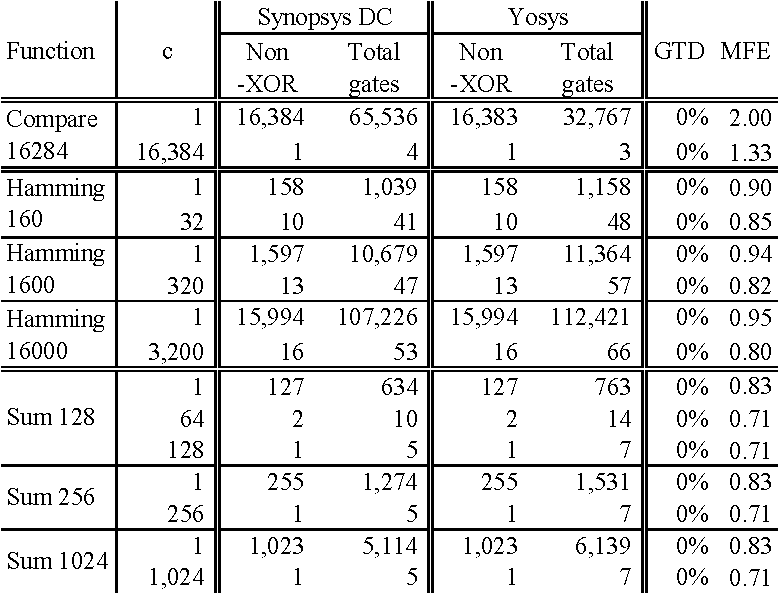
\includegraphics[width=0.7\textwidth]{abc-crop.pdf}
\end{table}


\pagebreak
\printglossary

\bibliographystyle{ieeetr}
\bibliography{main_bib}
\end{document}
